\documentclass[a4paper, pdf, twoside]{book}
\usepackage{iesbbook}
\geometry{a4paper,total={170mm,257mm},left=30mm,right=23mm,top=35mm,bottom=30mm, headsep=35pt}
\begin{document}
\thispagestyle{empty}
\pagestyle{plain}
\renewcommand{\headrulewidth}{0pt}
\begin{center}
\vspace*{0.5cm}\hrule\vspace{0.5cm}
\Huge \textbf{Matemàtiques 3r ESO} \par
\large \textit{Sèrie Pràctica}\par
\vspace{0.5cm}\hrule\vspace{0.5cm}
\Huge \textbf{\textsc{Solucionari}} \par \vspace{1.5cm}
	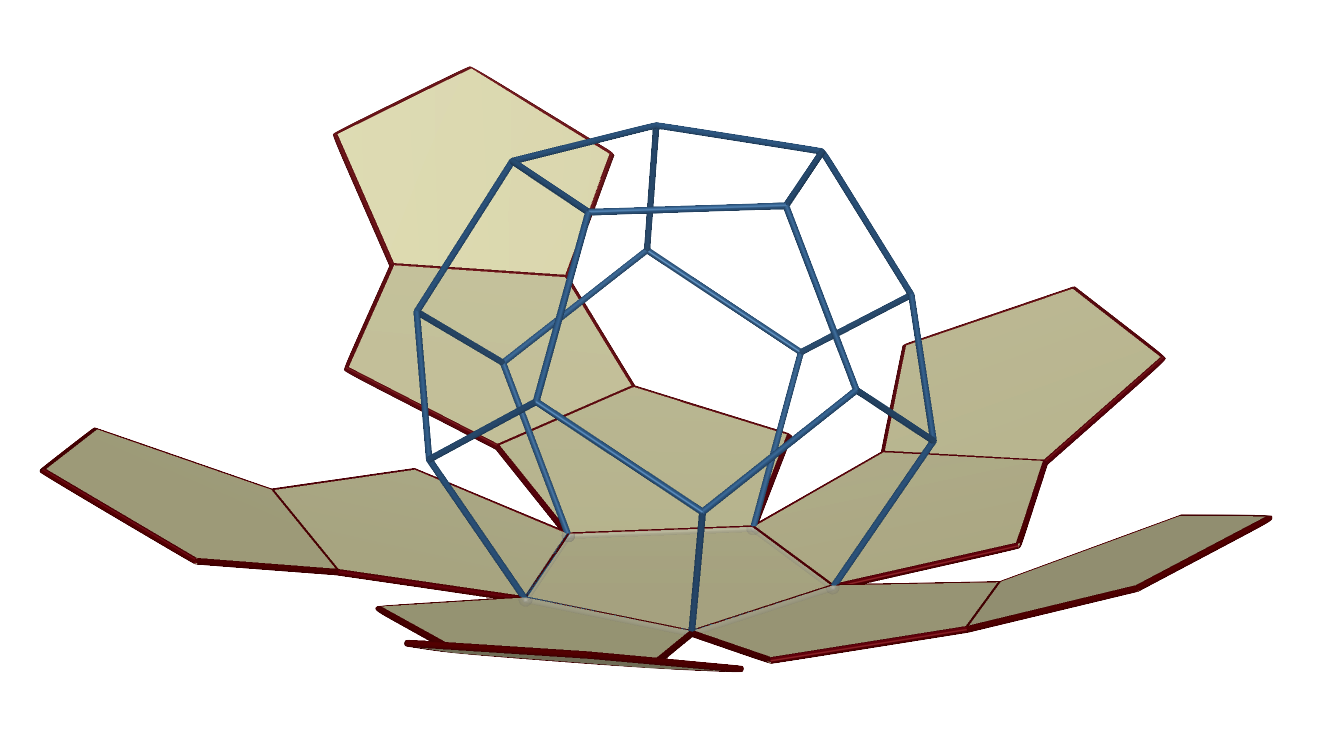
\includegraphics[width=0.9\textwidth]{img-00/portada}   

	\vspace{1.5cm}  
	\begin{minipage}{0.4\textwidth}  
		\begin{center}  
			\includegraphics*[width=1.2in]{img-00/ies-binissalem-logo}  
			\small  
			\noindent \href{www.iesbinissalem.net}{\textbf{www.iesbinissalem.net}}  
		\end{center}  
	\end{minipage}  
	\begin{minipage}{0.4\textwidth}  
		\begin{flushright}  
			\normalsize \textbf{Josep Mulet}\par 
			\textit{Departament de Matemàtiques}\par   
			IES Binissalem  
		\end{flushright}  
	\end{minipage}   
	\end{center}   
\cleartorightpage
\renewcommand{\baselinestretch}{1.5}
\tableofcontents \cleartorightpage
\renewcommand{\baselinestretch}{1}
\def\currentname{}
\pagestyle{fancy}
\renewcommand{\headrulewidth}{0.5pt}
\fancyhead[LE,RO]{\large\textcolor{darkBlueColor}{\shadowbox{\fontfamily{phv}\selectfont\textbf{\, \thepage \,}}}}
\fancyhead[LO,RE]{{ \fontfamily{phv}\selectfont \textit{\currentname} }}
\fancyfoot{}
\begin{multicols}{2}
\def\currentname{Solucions del Tema 1}
\vspace*{0.75cm}

 
 \needspace{5\baselineskip} 
 \scalebox{1.25}{\heading{Solucions del Tema 1}}

\vspace*{0.4cm}
\phantomsection \addcontentsline{toc}{section}{Solucions del Tema 1}
\vspace{0.3cm}

 \needspace{4\baselineskip} 

{\textbf{\em Pàgina 8}} \hrulefill
\begin{enumerate}
\vspace{0.25cm}
 \item[$\bullet$ ] {\fontfamily{phv}\selectfont\color{blue}\textbf{Avaluació inicial}. }
$a$: numerador,\par $b$: denominador,\par irreductible,\par $\frac {2}{3} \text { de } 24=16$,\par $\frac {3}{8}=0.375$ litres,\par \begin{tasks}(2) \task $\frac {5}{4}$ \task $2$ \task $\frac {3}{14}$ \task $18$ \end{tasks} 
 \end{enumerate}
\vspace{0.3cm}

 \needspace{4\baselineskip} 

{\textbf{\em Pàgina 9}} \hrulefill
\begin{enumerate}
\vspace{0.25cm}


 \needspace{2\baselineskip} 

 \item[\fontfamily{phv}\selectfont\color{blue}\textbf{1}. ] 
 \begin{tasks}[column-sep=1em, item-indent=1.3333em](2)
	 \task $10$
	 \task $-1$
	 \task $1215$
\end{tasks}
 \end{enumerate}
\begin{enumerate}
\vspace{0.25cm}
\item[\fontfamily{phv}\selectfont\color{blue}\textbf{2. }] 
$-1$
\vspace{0.25cm}


 \needspace{2\baselineskip} 

 \item[\fontfamily{phv}\selectfont\color{blue}\textbf{3}. ] 
 \begin{tasks}[column-sep=1em, item-indent=1.3333em](2)
	 \task $-14$
	 \task $-25$
\end{tasks}
\vspace{0.25cm}


 \needspace{2\baselineskip} 

 \item[\fontfamily{phv}\selectfont\color{blue}\textbf{4}. ]  \scalebox{0.6}{\simbolclau } 
 \begin{tasks}[column-sep=1em, item-indent=1.3333em](2)
	 \task $7$
	 \task $2$
	 \task $-3$
	 \task $-26$
\end{tasks}
 \end{enumerate}
\vspace{0.3cm}

 \needspace{4\baselineskip} 

{\textbf{\em Pàgina 10}} \hrulefill
\begin{enumerate}
\vspace{0.25cm}


 \needspace{2\baselineskip} 

 \item[\fontfamily{phv}\selectfont\color{blue}\textbf{5}. ]  \scalebox{0.6}{\simbolclau } 
 \begin{tasks}[column-sep=1em, item-indent=1.3333em](2)
	 \task $\frac {3}{5}$
	 \task $\frac {1}{9}$
	 \task $\frac {1}{12}$
	 \task $\frac {1}{4}$
\end{tasks}
 \end{enumerate}
\begin{enumerate}
\vspace{0.25cm}


 \needspace{2\baselineskip} 

 \item[\fontfamily{phv}\selectfont\color{blue}\textbf{6}. ]  \scalebox{0.6}{\simbolclau } 
 \begin{tasks}[column-sep=1em, item-indent=1.3333em](2)
	 \task $1$
	 \task $\frac {11}{6}$
	 \task $\frac {17}{14}$
	 \task $\frac {7}{15}$
	 \task $\frac {31}{20}$
	 \task $-\frac {1}{8}$
	 \task $\frac {1}{4}$
	 \task $\frac {41}{24}$
\end{tasks}
 \end{enumerate}
\vspace{0.3cm}

 \needspace{4\baselineskip} 

{\textbf{\em Pàgina 11}} \hrulefill
\begin{enumerate}
\vspace{0.25cm}


 \needspace{2\baselineskip} 

 \item[\fontfamily{phv}\selectfont\color{blue}\textbf{7}. ]  \scalebox{0.6}{\simbolclau } 
 \begin{tasks}[column-sep=1em, item-indent=1.3333em](2)
	 \task $\frac {2}{3}$
	 \task $8$
	 \task $\frac {1}{3}$
	 \task $\frac {1}{2}$
	 \task $\frac {1}{2}$
	 \task $1$
	 \task $\frac {5}{2}$
	 \task $2$
	 \task $-\frac {5}{6}$
	 \task $\frac {3}{2}$
	 \task $\frac {1}{3}$
	 \task $\frac {3}{5}$
\end{tasks}
 \end{enumerate}
\begin{enumerate}
\vspace{0.25cm}
\item[\fontfamily{phv}\selectfont\color{blue}\textbf{8. }] 
$\frac {3}{13}$
\vspace{0.25cm}
\item[\fontfamily{phv}\selectfont\color{blue}\textbf{9. }] 
$1$
\vspace{0.25cm}
\item[\fontfamily{phv}\selectfont\color{blue}\textbf{10. }] 
$0$
\vspace{0.25cm}


 \needspace{2\baselineskip} 

 \item[\fontfamily{phv}\selectfont\color{blue}\textbf{11}. ] 
 \begin{tasks}[column-sep=1em, item-indent=1.3333em](2)
	 \task $1$
	 \task $\frac {1}{2}$
\end{tasks}
\vspace{0.25cm}


 \needspace{2\baselineskip} 

 \item[\fontfamily{phv}\selectfont\color{blue}\textbf{12}. ]  \scalebox{0.6}{\simbolclau } 
 \begin{tasks}[column-sep=1em, item-indent=1.3333em](2)
	 \task $\frac {67}{4}$
	 \task $\frac {25}{4}$
	 \task $\frac {47}{8}$
\end{tasks}
 \end{enumerate}
\vspace{0.3cm}

 \needspace{4\baselineskip} 

{\textbf{\em Pàgina 12}} \hrulefill
\begin{enumerate}
\vspace{0.25cm}


 \needspace{2\baselineskip} 

 \item[\fontfamily{phv}\selectfont\color{blue}\textbf{13}. ] 
 \begin{tasks}[column-sep=1em, item-indent=1.3333em](2)
	 \task $7+\frac {1}{7}$
	 \task $2+\frac {3}{11}$
	 \task $16+\dfrac {5}{6}$
\end{tasks}
 \end{enumerate}
\begin{enumerate}
\vspace{0.25cm}


 \needspace{2\baselineskip} 

 \item[\fontfamily{phv}\selectfont\color{blue}\textbf{14}. ] 
 \begin{tasks}[column-sep=1em, item-indent=1.3333em](2)
	 \task $-4-\dfrac {2}{7}$
	 \task $-3-\dfrac {11}{13}$
	 \task $-4-\dfrac {16}{21}$
\end{tasks}
\vspace{0.25cm}
\item[\fontfamily{phv}\selectfont\color{blue}\textbf{15. }] 
Gràfica:\par 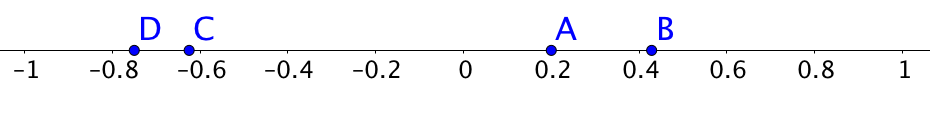
\includegraphics [width=0.45\textwidth ]{img-sol/t1-recta1}
\vspace{0.25cm}
\item[\fontfamily{phv}\selectfont\color{blue}\textbf{16. }] 
Gràfica:\par 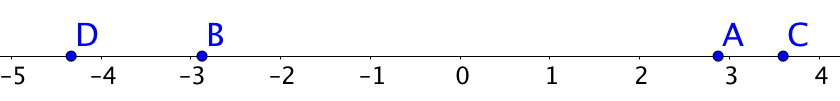
\includegraphics [width=0.45\textwidth ]{img-sol/t1-recta2}
 \end{enumerate}
\vspace{0.3cm}

 \needspace{4\baselineskip} 

{\textbf{\em Pàgina 13}} \hrulefill
\begin{enumerate}
\vspace{0.25cm}
\item[\fontfamily{phv}\selectfont\color{blue}\textbf{17. }] 
$A=-2-\dfrac {2}{9}=-\dfrac {20}{9}$;\par $B=-1-\dfrac {6}{8}=-\dfrac {14}{6}$;\par $C=-\dfrac {3}{4}$;\par $D=\dfrac {3}{5}$;\par $E=2+\dfrac {4}{7}=\dfrac {18}{7}$
 \end{enumerate}
\begin{enumerate}
\vspace{0.25cm}


 \needspace{2\baselineskip} 

 \item[\fontfamily{phv}\selectfont\color{blue}\textbf{18}. ] 
 \begin{tasks}[column-sep=1em, item-indent=1.3333em](2)
	 \task Exacte
	 \task Periòdic
	 \task Periòdic
	 \task Exacte
\end{tasks}
\vspace{0.25cm}


 \needspace{2\baselineskip} 

 \item[\fontfamily{phv}\selectfont\color{blue}\textbf{19}. ] 
 \begin{tasks}[column-sep=1em, item-indent=1.3333em](2)
	 \task $\dfrac {7071}{5000}$
	 \task $\dfrac {1}{8}$
	 \task $\dfrac {333}{50}$
\end{tasks}
\vspace{0.25cm}


 \needspace{2\baselineskip} 

 \item[\fontfamily{phv}\selectfont\color{blue}\textbf{20}. ] 
 \begin{tasks}[column-sep=1em, item-indent=1.3333em](2)
	 \task $\dfrac {14141}{9999}$
	 \task $\dfrac {125}{999}$
	 \task $\dfrac {20}{3}$
\end{tasks}
\vspace{0.25cm}


 \needspace{2\baselineskip} 

 \item[\fontfamily{phv}\selectfont\color{blue}\textbf{21}. ] 
 \begin{tasks}[column-sep=1em, item-indent=1.3333em](2)
	 \task $\dfrac {47}{45}$
	 \task $\dfrac {3559}{4995}$
	 \task $\dfrac {203}{50}$
\end{tasks}
 \end{enumerate}
\vspace{0.3cm}

 \needspace{4\baselineskip} 

{\textbf{\em Pàgina 14}} \hrulefill
\begin{enumerate}
\vspace{0.25cm}
\item[\fontfamily{phv}\selectfont\color{blue}\textbf{22. }] 
 {\renewcommand {\arraystretch }{1.8} \begin {tabular}{|c|c|c|} \hline \rowcolor {lightgray} Decimal & Fracció & \% \\ \hline 0,75 & $\frac {3}{4}$ & 75 \% \\ \hline 1,5 & $\frac {6}{4}$ & 150 \% \\ \hline 0,58 & $\frac {17}{25}$ & 68\% \\ \hline \end {tabular}} 
 \end{enumerate}
\begin{enumerate}
\vspace{0.25cm}
\item[\fontfamily{phv}\selectfont\color{blue}\textbf{23. }] 
$130$ \%=$0.13$ i $\frac {7}{25}=28$ \%
\vspace{0.25cm}


 \needspace{2\baselineskip} 

 \item[\fontfamily{phv}\selectfont\color{blue}\textbf{24}. ]  \scalebox{0.6}{\simbolclau } 
 \begin{tasks}[column-sep=1em, item-indent=1.3333em](3)
	 \task $1$
	 \task $\dfrac {20}{9}$
	 \task $\dfrac {99}{100}$
\end{tasks}
\vspace{0.25cm}
\item[\fontfamily{phv}\selectfont\color{blue}\textbf{25. }] 
$4,999{\cdots }=4,\hat {9}=\frac {49-4}{9}=\frac {45}{9}=5$.\par En general: $n,999{\cdots }=n,\hat {9}=\frac {10n+9-n}{9}=\frac {9n+9}{9}=n+1$ 
\vspace{0.25cm}
\item[\fontfamily{phv}\selectfont\color{blue}\textbf{26. }] 
Gràfica:\par 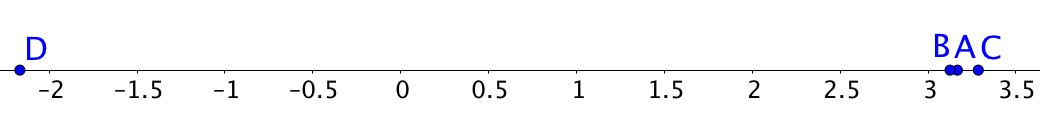
\includegraphics [width=0.5\textwidth ]{img-sol/t1-recta3}
 \end{enumerate}
\vspace{0.3cm}

 \needspace{4\baselineskip} 

{\textbf{\em Pàgina 15}} \hrulefill
\begin{enumerate}
\vspace{0.25cm}
\item[\fontfamily{phv}\selectfont\color{blue}\textbf{28. }] 
$\frac {-9}{8}< \frac {-8}{9}<\frac {4}{5} <\frac {38}{45} <\frac {77}{90} < \frac {8}{9}$
 \end{enumerate}
\begin{enumerate}
\vspace{0.25cm}
\item[\fontfamily{phv}\selectfont\color{blue}\textbf{29. }] 
$-\frac {7}{4}<-\frac {5}{3}<-\frac {1}{6}<\frac {3}{8}<\frac {5}{12}<\frac {11}{24}$
\vspace{0.25cm}
\item[\fontfamily{phv}\selectfont\color{blue}\textbf{30. }] 
El que començam fent és sumar les dues fraccions $a$ i $b$. Després el resultat en dividim entre dos. D'aquesta forma tenim el nombre que està enmig. Per exemple: si $a=\frac {2}{3}$ i $b=\frac {5}{4}$, \[\frac {2}{3} +\frac {5}{4} =\frac {8}{12} + \frac {}{12} = \frac {23}{12} \] Finalment dividim entre dos: La fracció és $ \frac {23}{24} \approx 0,958\hat {3}$ \par 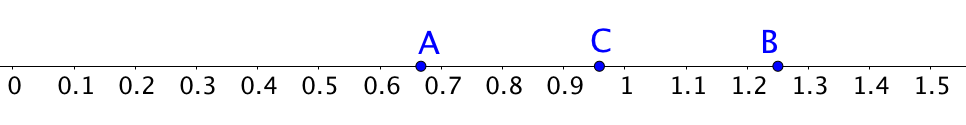
\includegraphics [width=0.5\textwidth ]{img-sol/t1-recta4} 
\vspace{0.25cm}
\item[\fontfamily{phv}\selectfont\color{blue}\textbf{31. }] 
80
\vspace{0.25cm}
\item[\fontfamily{phv}\selectfont\color{blue}\textbf{32. }] 
390
\vspace{0.25cm}
\item[\fontfamily{phv}\selectfont\color{blue}\textbf{33. }] 
32 pots
\vspace{0.25cm}
\item[\fontfamily{phv}\selectfont\color{blue}\textbf{34. }] 
Per exemple: En el nostre institut les $\frac {2}{5}$ parts dels alumnes de 3r d'ESO són d'Alaró. Si en total hi ha $200$ alumnes a 3r d'ESO, quants són d'Alaró?\par \par Solució: $\frac {2}{5}$ de $200$ = 80 alumnes són d'Alaró.
 \end{enumerate}
\vspace{0.3cm}

 \needspace{4\baselineskip} 

{\textbf{\em Pàgina 16}} \hrulefill
\begin{enumerate}
\vspace{0.25cm}


 \needspace{2\baselineskip} 

 \item[\fontfamily{phv}\selectfont\color{blue}\textbf{35}. ] 
 \begin{tasks}[column-sep=1em, item-indent=1.3333em](2)
	 \task 65.024 cm
	 \task 86.6986 cm
\end{tasks}
 \end{enumerate}
\begin{enumerate}
\vspace{0.25cm}
\item[\fontfamily{phv}\selectfont\color{blue}\textbf{36. }] 
$77,7...= \dfrac {700}{9}$; Són 36 alumnes en total dels quals aproven 28
\vspace{0.25cm}
\item[\fontfamily{phv}\selectfont\color{blue}\textbf{37. }] 
Perden 8 partits (10 empatats). $\dfrac {6}{24}=25$ \%
\vspace{0.25cm}
\item[\fontfamily{phv}\selectfont\color{blue}\textbf{38. }] 
Total 24000 \euro {}; 1r: 12000 \euro {}, 2n: 8000 \euro {}, 3r: 2000 \euro {} 
\vspace{0.25cm}
\item[\fontfamily{phv}\selectfont\color{blue}\textbf{39. }] 
645 nines + 376 nins = 1021 alumnes practiquen natació.
\vspace{0.25cm}


 \needspace{2\baselineskip} 

 \item[\fontfamily{phv}\selectfont\color{blue}\textbf{40}. ] 
 \begin{tasks}[column-sep=1em, item-indent=1.3333em](2)
	 \task $\dfrac {3}{20}=15$ \%
	 \task $12960$ \euro {}
\end{tasks}
\vspace{0.25cm}
\item[\fontfamily{phv}\selectfont\color{blue}\textbf{41. }] 
La caixa conté 60 llepolies. Primer fill 30, segon fill 24 llepolies.
 \end{enumerate}
\vspace{0.3cm}

 \needspace{4\baselineskip} 

{\textbf{\em Pàgina 17}} \hrulefill
\begin{enumerate}
\vspace{0.25cm}
\item[\fontfamily{phv}\selectfont\color{blue}\textbf{42. }] 
100 \euro {}
 \end{enumerate}
\begin{enumerate}
\vspace{0.25cm}


 \needspace{2\baselineskip} 

 \item[\fontfamily{phv}\selectfont\color{blue}\textbf{43}. ] 
 \begin{tasks}[column-sep=1em, item-indent=1.3333em](2)
	 \task 7/39
	 \task Es van presentar 312 aspirants
\end{tasks}
\vspace{0.25cm}


 \needspace{2\baselineskip} 

 \item[\fontfamily{phv}\selectfont\color{blue}\textbf{44}. ] 
 \begin{tasks}[column-sep=1em, item-indent=1.3333em](2)
	 \task 7/15
	 \task 1.560.000 \euro {}
\end{tasks}
\vspace{0.25cm}


 \needspace{2\baselineskip} 

 \item[\fontfamily{phv}\selectfont\color{blue}\textbf{45}. ] 
 \begin{tasks}[column-sep=1em, item-indent=1.3333em](2)
	 \task 1/8
	 \task 90; 45; 54; 27 cada setmana
\end{tasks}
\vspace{0.25cm}
\item[\fontfamily{phv}\selectfont\color{blue}\textbf{46. }] 
48 botelles
\vspace{0.25cm}
\item[\fontfamily{phv}\selectfont\color{blue}\textbf{47. }] 
$2\times 3\times 4\times 5\times 6\times 7=5040$ o també 420.
\vspace{0.25cm}
\item[\fontfamily{phv}\selectfont\color{blue}\textbf{48. }] 
Cal multiplicar per la fracció $\dfrac {5}{3}$
\vspace{0.25cm}


 \needspace{2\baselineskip} 

 \item[\fontfamily{phv}\selectfont\color{blue}\textbf{49}. ] 
 \begin{tasks}[column-sep=1em, item-indent=1.3333em](2)
	 \task $\dfrac {8}{9}$
	 \task $\dfrac {8}{9}$
\end{tasks}
\vspace{0.25cm}
\item[\fontfamily{phv}\selectfont\color{blue}\textbf{50. }] 
2/3 de metre.
 \end{enumerate}
\vspace{0.3cm}

 \needspace{4\baselineskip} 

{\textbf{\em Pàgina 18}} \hrulefill
\begin{enumerate}
\vspace{0.25cm}
\item[\fontfamily{phv}\selectfont\color{blue}\textbf{51. }] 

\mbox{}
 \scalebox{0.5}{\begin {tabular}{|p{0.15\textwidth }|p{0.15\textwidth }|p{0.15\textwidth }|p{0.15\textwidth }|p{0.15\textwidth }|} \hline \textbf {} & \multicolumn {4}{|p{0.6\textwidth }|}{Xifres significatives} \\ \hline \textbf {Nombre} & 1 & 2 & 3 & 4 \\ \hline \textbf {$\sqrt {10} $} & 3 & 3.2 & 3.16 & 3.162 \\ \hline \textbf {1/7} & 0.1 & 0.14 & 0.143 & 0.1429 \\ \hline \textbf {95549} & 100000 & 96000 & 95500 & 95550\\ \hline \textbf {30000} & 3·10${}^{4}$ & 30·10${}^{3}$ & 300·10${}^{2}$ & 3000·10${}^{1}$ \\ \hline \textbf {1,9995} & 2 & 2,0 & 2,00 & 2,000 \\ \hline \end {tabular}} 
 \end{enumerate}
\begin{enumerate}
\vspace{0.25cm}
\item[\fontfamily{phv}\selectfont\color{blue}\textbf{52. }] 
Els dos tenen com $E_R=4.05\cdot 10^{-3}$
\vspace{0.25cm}


 \needspace{2\baselineskip} 

 \item[\fontfamily{phv}\selectfont\color{blue}\textbf{53}. ] 
 \begin{tasks}[column-sep=1em, item-indent=1.3333em](2)
	 \task Depèn si $E_R$ o $E_A$
	 \task F
	 \task V
	 \task F
	 \task F
	 \task V
\end{tasks}
\vspace{0.25cm}
\item[\fontfamily{phv}\selectfont\color{blue}\textbf{54. }] 
$32567=33000$ amb $E_R=0.013$ i $1,395=1,400$ amb $E_R=0.0036$
\vspace{0.25cm}
\item[\fontfamily{phv}\selectfont\color{blue}\textbf{55. }] 
$3.1416 = \dfrac {31416}{10000}=\dfrac {3927}{1250}$
\vspace{0.25cm}


 \needspace{2\baselineskip} 

 \item[\fontfamily{phv}\selectfont\color{blue}\textbf{56}. ] 
 \begin{tasks}[column-sep=1em, item-indent=1.3333em](2)
	 \task $\dfrac {355}{113}$
	 \task $E_A=2.67\cdot 10^{-7}$
	 \task $E_R=8.5\cdot 10^{-6}$
\end{tasks}
 \end{enumerate}
\vspace{0.3cm}

 \needspace{4\baselineskip} 

{\textbf{\em Pàgina 19}} \hrulefill
\begin{enumerate}
\vspace{0.25cm}
 \item[$\bullet$ ] {\fontfamily{phv}\selectfont\color{blue}\textbf{Autoavaluació:}. }

 \end{enumerate}
\begin{enumerate}
\vspace{0.25cm}
\item[\fontfamily{phv}\selectfont\color{blue}\textbf{1. }]  \scalebox{0.6}{\simbolclau } 
10
\vspace{0.25cm}
\item[\fontfamily{phv}\selectfont\color{blue}\textbf{2. }]  \scalebox{0.6}{\simbolclau } 
$\frac {7}{8}>\frac {5}{6}>\frac {-5}{6}>\frac {-7}{8}>\frac {-5}{4}$
\vspace{0.25cm}
\item[\fontfamily{phv}\selectfont\color{blue}\textbf{4. }]  \scalebox{0.6}{\simbolclau } 
$\frac {7}{2}$
\vspace{0.25cm}


 \needspace{2\baselineskip} 

 \item[\fontfamily{phv}\selectfont\color{blue}\textbf{5}. ]  \scalebox{0.6}{\simbolclau } 
 \begin{tasks}[column-sep=1em, item-indent=1.3333em](2)
	 \task 180
	 \task 960 cm${}^3$
\end{tasks}
\vspace{0.25cm}


 \needspace{2\baselineskip} 

 \item[\fontfamily{phv}\selectfont\color{blue}\textbf{6}. ]  \scalebox{0.6}{\simbolclau } 
 \begin{tasks}[column-sep=1em, item-indent=1.3333em](1)
	 \task 9900,$E_A$=41,$E_R$=0.42\%
	 \task 9.9,$E_A$=0.045,$E_R$=0,45\% 
\end{tasks}
\vspace{0.25cm}


 \needspace{2\baselineskip} 

 \item[\fontfamily{phv}\selectfont\color{blue}\textbf{7}. ]  \scalebox{0.6}{\simbolclau } 
 \begin{tasks}[column-sep=1em, item-indent=1.3333em](2)
	 \task* Són exactes $\dfrac {6}{120}$ i $\dfrac {42}{150}$. $\dfrac {5}{180}$ és decimal periòdic
	 \task 10 xifres
	 \task 96 xifres
\end{tasks}
\vspace{0.25cm}
\item[\fontfamily{phv}\selectfont\color{blue}\textbf{8. }]  \scalebox{0.6}{\simbolclau } 
$\frac {89}{40}$, $\frac {2203}{990}$, $\frac {999}{1000}=0,999$
\vspace{0.25cm}


 \needspace{2\baselineskip} 

 \item[\fontfamily{phv}\selectfont\color{blue}\textbf{9}. ]  \scalebox{0.6}{\simbolclau } 
 \begin{tasks}[column-sep=1em, item-indent=1.3333em](2)
	 \task 4 setmanes
	 \task 506.25 cm${}^{3}$
\end{tasks}
\vspace{0.25cm}
\item[\fontfamily{phv}\selectfont\color{blue}\textbf{10. }]  \scalebox{0.6}{\simbolclau } 
Cobrava 1200 \euro {}. Ara cobra 1000 \euro {}, paga 250 \euro {} d'impostos i 300 \euro {} d'hipoteca. 
 \end{enumerate}
\vfill\null
\columnbreak
\def\currentname{Solucions del Tema 2}
\vspace*{0.75cm}

 
 \needspace{5\baselineskip} 
 \scalebox{1.25}{\heading{Solucions del Tema 2}}

\vspace*{0.4cm}
\phantomsection \addcontentsline{toc}{section}{Solucions del Tema 2}
\vspace{0.3cm}

 \needspace{4\baselineskip} 

{\textbf{\em Pàgina 22}} \hrulefill
\begin{enumerate}
\vspace{0.25cm}
 \item[$\bullet$ ] {\fontfamily{phv}\selectfont\color{blue}\textbf{Avaluació inicial}. }
base;\par exponent;\par sumam;\par restam; \par multiplicam.\par \begin{tasks}(2) \task --8 \task 16 \task 1 \task 12 \task $\frac {1}{4}$ \task 2 \task $5^{12}$ \task $(-3)^3$ \task $7^{15}$ \end{tasks} 
 \end{enumerate}
\vspace{0.3cm}

 \needspace{4\baselineskip} 

{\textbf{\em Pàgina 23}} \hrulefill
\begin{enumerate}
\vspace{0.25cm}


 \needspace{2\baselineskip} 

 \item[\fontfamily{phv}\selectfont\color{blue}\textbf{1}. ] 
 \begin{tasks}[column-sep=1em, item-indent=1.3333em](2)
	 \task Negatiu
	 \task Positiu
	 \task Negatiu
	 \task Positiu
\end{tasks}
 \end{enumerate}
\begin{enumerate}
\vspace{0.25cm}


 \needspace{2\baselineskip} 

 \item[\fontfamily{phv}\selectfont\color{blue}\textbf{2}. ] 
 \begin{tasks}[column-sep=1em, item-indent=1.3333em](2)
	 \task $81$
	 \task $-8$
	 \task $-1$
	 \task $-4$
\end{tasks}
\vspace{0.25cm}


 \needspace{2\baselineskip} 

 \item[\fontfamily{phv}\selectfont\color{blue}\textbf{3}. ] 
 \begin{tasks}[column-sep=1em, item-indent=1.3333em](2)
	 \task $\dfrac {81}{16}$
	 \task $\dfrac {1}{125}$
	 \task $1$
	 \task $-\dfrac {27}{64}$
\end{tasks}
\vspace{0.25cm}


 \needspace{2\baselineskip} 

 \item[\fontfamily{phv}\selectfont\color{blue}\textbf{4}. ] 
 \begin{tasks}[column-sep=1em, item-indent=1.3333em](2)
	 \task $-\dfrac {1}{3}$
	 \task $\dfrac {1}{2}$
	 \task $-4$
	 \task $\dfrac {7}{4}$
\end{tasks}
 \end{enumerate}
\vspace{0.3cm}

 \needspace{4\baselineskip} 

{\textbf{\em Pàgina 24}} \hrulefill
\begin{enumerate}
\vspace{0.25cm}


 \needspace{2\baselineskip} 

 \item[\fontfamily{phv}\selectfont\color{blue}\textbf{5}. ] 
 \begin{tasks}[column-sep=1em, item-indent=1.3333em](2)
	 \task $-\dfrac {1}{27}$
	 \task $\dfrac {1}{16}$
	 \task $16$
	 \task $\dfrac {343}{64}$
	 \task $\dfrac {125}{64}$
	 \task $-\dfrac {2041}{16}$
	 \task $1296$
	 \task $\dfrac {4}{25}$
\end{tasks}
 \end{enumerate}
\begin{enumerate}
\vspace{0.25cm}


 \needspace{2\baselineskip} 

 \item[\fontfamily{phv}\selectfont\color{blue}\textbf{6}. ] 
 \begin{tasks}[column-sep=1em, item-indent=1.3333em](2)
	 \task $(-7)^{16}$
	 \task $3^{17}$
	 \task $120^4$
	 \task $8^6$
	 \task $(-3)^{-3}$
	 \task $(-25)^4$
	 \task $(-5/8)^8$
	 \task $(-2)^{30}$
\end{tasks}
\vspace{0.25cm}


 \needspace{2\baselineskip} 

 \item[\fontfamily{phv}\selectfont\color{blue}\textbf{7}. ] 
 \begin{tasks}[column-sep=1em, item-indent=1.3333em](2)
	 \task* $\left (-\frac {4}{3} \right )^{2}$
	 \task* $\left (\frac {1}{8} \right )^{-3}=8^3$
	 \task* $\left (\frac {5}{42} \right )^6$
	 \task* $\left (\frac {160}{9} \right )^4$
	 \task* $\left (-\frac {5}{2} \right )^3$
	 \task* $\left (\frac {5}{8} \right )^5$
	 \task* $\left (\frac {10}{9} \right )^3$
	 \task $27^5$
\end{tasks}
 \end{enumerate}
\vspace{0.3cm}

 \needspace{4\baselineskip} 

{\textbf{\em Pàgina 25}} \hrulefill
\begin{enumerate}
\vspace{0.25cm}


 \needspace{2\baselineskip} 

 \item[\fontfamily{phv}\selectfont\color{blue}\textbf{8}. ] 
 \begin{tasks}[column-sep=1em, item-indent=1.3333em](2)
	 \task $6^5$
	 \task $1$
	 \task $40^3$
	 \task $5^6$
	 \task $9^{10}$
	 \task $6^4$
	 \task $6^3$
	 \task $(-3)^{-2}$
\end{tasks}
 \end{enumerate}
\begin{enumerate}
\vspace{0.25cm}


 \needspace{2\baselineskip} 

 \item[\fontfamily{phv}\selectfont\color{blue}\textbf{9}. ] 
 \begin{tasks}[column-sep=1em, item-indent=1.3333em](2)
	 \task $\left (\frac {-1}{4}\right )^3$
	 \task $\left (\frac {1}{9}\right )^3$
	 \task $\left (\frac {1}{2}\right )^4$
	 \task $\left (\frac {-1}{5}\right )^3$
\end{tasks}
\vspace{0.25cm}


 \needspace{2\baselineskip} 

 \item[\fontfamily{phv}\selectfont\color{blue}\textbf{10}. ] 
 \begin{tasks}[column-sep=1em, item-indent=1.3333em](2)
	 \task $\left (\frac {4}{135}\right )^3$
	 \task $\left (-\frac {1}{4}\right )^6$
	 \task $\left (\frac {-2}{15}\right )^6$
	 \task $\left (\frac {2}{5}\right )^{12/12}=\frac {2}{5}$
\end{tasks}
 \end{enumerate}
\vspace{0.3cm}

 \needspace{4\baselineskip} 

{\textbf{\em Pàgina 26}} \hrulefill
\begin{enumerate}
\vspace{0.25cm}


 \needspace{2\baselineskip} 

 \item[\fontfamily{phv}\selectfont\color{blue}\textbf{11}. ] 
 \begin{tasks}[column-sep=1em, item-indent=1.3333em](2)
	 \task $\cient {1.4}{8}$
	 \task $\cient {3.28}{4}$
	 \task $\cient {7.1}{16}$
	 \task $\cient {7.5}{-6}$
	 \task $\cient {-1.8}{7}$
	 \task $\cient {4.2}{-10}$
	 \task $\cient {-9}{-3}$
	 \task $\cient {7}{-11}$
\end{tasks}
 \end{enumerate}
\begin{enumerate}
\vspace{0.25cm}


 \needspace{2\baselineskip} 

 \item[\fontfamily{phv}\selectfont\color{blue}\textbf{12}. ] 
 \begin{tasks}[column-sep=1em, item-indent=1.3333em](2)
	 \task $\cient {3.84}{8}$ m
	 \task $\cient {1.66}{-27}$ kg
	 \task $\cient {9.46}{12}$ km
	 \task $\cient {10}{100}$
\end{tasks}
\vspace{0.25cm}


 \needspace{2\baselineskip} 

 \item[\fontfamily{phv}\selectfont\color{blue}\textbf{13}. ]  \scalebox{0.6}{\simbolclau } 
 \begin{tasks}[column-sep=1em, item-indent=1.3333em](2)
	 \task $2.231\cdot 10^6$
	 \task $5.678\cdot 10^{-3}$
	 \task $1.35\cdot 10^{-5}$
	 \task $3.6\cdot 10^{-4}$
\end{tasks}
\vspace{0.25cm}
\item[\fontfamily{phv}\selectfont\color{blue}\textbf{14. }]  \scalebox{0.6}{\simbolclau } 
$1.629\cdot 10^{17}$ m
\vspace{0.25cm}
\item[\fontfamily{phv}\selectfont\color{blue}\textbf{15. }]  \scalebox{0.6}{\simbolclau } 
La massa de l'isòtop C${}_{14}$ és: $6\times 1,672 \cdot 10^{-27} + 6 \times 9,11 \cdot 10^{-31}+ 8\times 1,64 \cdot 10^{-27} = 2.32\cdot 10^{-26}$ kg
 \end{enumerate}
\vspace{0.3cm}

 \needspace{4\baselineskip} 

{\textbf{\em Pàgina 27}} \hrulefill
\begin{enumerate}
\vspace{0.25cm}


 \needspace{2\baselineskip} 

 \item[\fontfamily{phv}\selectfont\color{blue}\textbf{16}. ] 
 \begin{tasks}[column-sep=1em, item-indent=1.3333em](2)
	 \task $\cient {1.236}{-2}$
	 \task $\cient {-2.33}{7}$
	 \task $\cient {-3.99}{2}$
	 \task $\cient {4.12}{-6}$
\end{tasks}
 \end{enumerate}
\begin{enumerate}
\vspace{0.25cm}
\item[\fontfamily{phv}\selectfont\color{blue}\textbf{17. }]  \scalebox{0.6}{\simbolclau } 
$50 t \cdot \frac {1\,000\,0000 \text { g}}{1 t} \cdot \frac {40\cdot 10^6 \text { bacteris}}{1 \text { g}}=4\cdot 10^{13}$ bacteris
\vspace{0.25cm}


 \needspace{2\baselineskip} 

 \item[\fontfamily{phv}\selectfont\color{blue}\textbf{18}. ] 
 \begin{tasks}[column-sep=1em, item-indent=1.3333em](2)
	 \task $\cient {1.392}{2}$
	 \task $\cient {4.86}{5}$
	 \task $\cient {7.2}{5}$
\end{tasks}
\vspace{0.25cm}
\item[\fontfamily{phv}\selectfont\color{blue}\textbf{19. }]  \scalebox{0.6}{\simbolclau } 
$ 598 \cdot 10^{25} \text { g} \cdot \frac {50 \text { grans}}{1 \text { g}} \approx 3\cdot 10^{29}$ grans d'arena
\vspace{0.25cm}
\item[\fontfamily{phv}\selectfont\color{blue}\textbf{20. }] 
$M_J=1,898$·$10^{27}$ kg, $M_T=5,972$·$10^{24}$ kg, $R_J=69911$ km, $R_T=6371$ km, \par a) $\dfrac {M_J}{M_T} = 318$,\par b) $\dfrac {V_J}{V_T} = 1321$, $\dfrac {d_J}{d_T} = 0.24$\par és un planeta gasós (de fet és menys dens que l'aigua).
\vspace{0.25cm}
\item[\fontfamily{phv}\selectfont\color{blue}\textbf{21. }] 
14 anys=$\cient {4.42}{8}$ s;\par 15 anys=$\cient {4.73}{8}$ s;\par 16 anys=$\cient {5.05}{8}$ s
\vspace{0.25cm}
\item[\fontfamily{phv}\selectfont\color{blue}\textbf{22. }] 
$\cient {1.2856}{9}$ km${}^{3}$ i $\cient {3.5}{7}$ km${}^{3}$.\par La proporció és 2.72 \%
\vspace{0.25cm}
\item[\fontfamily{phv}\selectfont\color{blue}\textbf{23. }] 
Si tenim present que l'electró, que pesa 9,109 $\cdot $ 10${}^{-}$${}^{31}$ kg, representa únicament l'1 \%, només cal multiplicar per 100 i obtenim la massa de l'àtom: $\cient {9.109}{-29}$ kg
\vspace{0.25cm}
\item[\fontfamily{phv}\selectfont\color{blue}\textbf{24. }] 
En Joan té $\cient {2.5}{9}$ glòbuls vermells
 \end{enumerate}
\vspace{0.3cm}

 \needspace{4\baselineskip} 

{\textbf{\em Pàgina 28}} \hrulefill
\begin{enumerate}
\vspace{0.25cm}
\item[\fontfamily{phv}\selectfont\color{blue}\textbf{25. }] 
1, 4, 9, 16, 25, 36, 49, 64, 81, 100
 \end{enumerate}
\begin{enumerate}
\vspace{0.25cm}


 \needspace{2\baselineskip} 

 \item[\fontfamily{phv}\selectfont\color{blue}\textbf{26}. ] 
 \begin{tasks}[column-sep=1em, item-indent=1.3333em](2)
	 \task 7
	 \task 5
	 \task 10
	 \task 8
	 \task 9
	 \task 1
	 \task 0
\end{tasks}
\vspace{0.25cm}


 \needspace{2\baselineskip} 

 \item[\fontfamily{phv}\selectfont\color{blue}\textbf{27}. ] 
 \begin{tasks}[column-sep=1em, item-indent=1.3333em](2)
	 \task 7
	 \task 5
	 \task 10
	 \task 7
	 \task 8
	 \task 1
	 \task 11
\end{tasks}
 \end{enumerate}
\vspace{0.3cm}

 \needspace{4\baselineskip} 

{\textbf{\em Pàgina 29}} \hrulefill
\begin{enumerate}
\vspace{0.25cm}


 \needspace{2\baselineskip} 

 \item[\fontfamily{phv}\selectfont\color{blue}\textbf{28}. ] 
 \begin{tasks}[column-sep=1em, item-indent=1.3333em](2)
	 \task entera
	 \task no
	 \task natural
	 \task irracional
	 \task irracional
	 \task irracional
	 \task entera
	 \task entera
\end{tasks}
 \end{enumerate}
\begin{enumerate}
\vspace{0.25cm}


 \needspace{2\baselineskip} 

 \item[\fontfamily{phv}\selectfont\color{blue}\textbf{29}. ] 
 \begin{tasks}[column-sep=1em, item-indent=1.3333em](2)
	 \task $\pm 11$
	 \task --2
	 \task $\pm 10$
	 \task --1
	 \task 1
\end{tasks}
\vspace{0.25cm}


 \needspace{2\baselineskip} 

 \item[\fontfamily{phv}\selectfont\color{blue}\textbf{30}. ] 
 \begin{tasks}[column-sep=1em, item-indent=1.3333em](2)
	 \task $\sqrt [5]{(-3)^4}$
	 \task $\sqrt [3]{8}$
	 \task $\sqrt [3]{5^2}$
\end{tasks}
\vspace{0.25cm}


 \needspace{2\baselineskip} 

 \item[\fontfamily{phv}\selectfont\color{blue}\textbf{31}. ] 
 \begin{tasks}[column-sep=1em, item-indent=1.3333em](2)
	 \task $\sqrt [5]{(-4)^3}$
	 \task $\sqrt [6]{7}$
	 \task $\sqrt [3]{21}$
	 \task $\sqrt [3]{(-5)^2}$
\end{tasks}
\vspace{0.25cm}


 \needspace{2\baselineskip} 

 \item[\fontfamily{phv}\selectfont\color{blue}\textbf{32}. ] 
 \begin{tasks}[column-sep=1em, item-indent=1.3333em](2)
	 \task $6^{3/5}$
	 \task $(-7)^{5/2}$
	 \task $3^{5/2}$
	 \task $(-30)^{4/3}$
\end{tasks}
\vspace{0.25cm}


 \needspace{2\baselineskip} 

 \item[\fontfamily{phv}\selectfont\color{blue}\textbf{33}. ] 
 \begin{tasks}[column-sep=1em, item-indent=1.3333em](2)
	 \task 110
	 \task 0.8
	 \task --0.2
	 \task --1
	 \task 0.7
\end{tasks}
\vspace{0.25cm}


 \needspace{2\baselineskip} 

 \item[\fontfamily{phv}\selectfont\color{blue}\textbf{34}. ] 
 \begin{tasks}[column-sep=1em, item-indent=1.3333em](2)
	 \task 1.2
	 \task --0.1
	 \task 5800
	 \task --0.03
\end{tasks}
 \end{enumerate}
\vspace{0.3cm}

 \needspace{4\baselineskip} 

{\textbf{\em Pàgina 30}} \hrulefill
\begin{enumerate}
\vspace{0.25cm}


 \needspace{2\baselineskip} 

 \item[\fontfamily{phv}\selectfont\color{blue}\textbf{35}. ] 
 \begin{tasks}[column-sep=1em, item-indent=1.3333em](2)
	 \task $8\sqrt {2}$
	 \task $\frac {9}{2}\sqrt {5}$
	 \task* $\frac {7}{4}\sqrt {2}-2\sqrt {3}$
	 \task $-2\sqrt {7}+3\sqrt {3}$
\end{tasks}
 \end{enumerate}
\begin{enumerate}
\vspace{0.25cm}


 \needspace{2\baselineskip} 

 \item[\fontfamily{phv}\selectfont\color{blue}\textbf{36}. ]  \scalebox{0.6}{\simbolclau } 
 \begin{tasks}[column-sep=1em, item-indent=1.3333em](2)
	 \task $a\cdot b\,\sqrt [4]{a^2 b}$
	 \task* $6^2 \cdot 3 \cdot 2^2 \sqrt [3]{3\cdot 6^2}$
	 \task $90\,\sqrt {45}$
\end{tasks}
\vspace{0.25cm}


 \needspace{2\baselineskip} 

 \item[\fontfamily{phv}\selectfont\color{blue}\textbf{37}. ]  \scalebox{0.6}{\simbolclau } 
 \begin{tasks}[column-sep=1em, item-indent=1.3333em](2)
	 \task $5^3\,\sqrt [{3}]{5}$
	 \task $3\sqrt {6}$
	 \task $\frac {2}{3}\sqrt {2}$
	 \task $\frac {x}{y^2}\sqrt {x }$
\end{tasks}
 \end{enumerate}
\vspace{0.3cm}

 \needspace{4\baselineskip} 

{\textbf{\em Pàgina 31}} \hrulefill
\begin{enumerate}
\vspace{0.25cm}


 \needspace{2\baselineskip} 

 \item[\fontfamily{phv}\selectfont\color{blue}\textbf{38}. ] 
 \begin{tasks}[column-sep=1em, item-indent=1.3333em](2)
	 \task $\sqrt [6]{18}$
	 \task $\sqrt [12]{25}$
\end{tasks}
 \end{enumerate}
\begin{enumerate}
\vspace{0.25cm}


 \needspace{2\baselineskip} 

 \item[\fontfamily{phv}\selectfont\color{blue}\textbf{39}. ] 
 \begin{tasks}[column-sep=1em, item-indent=1.3333em](2)
	 \task $2^{13/4}=\sqrt [4]{2^{13}}$
	 \task $5^{-2/3}=\sqrt [3]{5^{-2}}$
\end{tasks}
\vspace{0.25cm}


 \needspace{2\baselineskip} 

 \item[\fontfamily{phv}\selectfont\color{blue}\textbf{40}. ] 
 \begin{tasks}[column-sep=1em, item-indent=1.3333em](2)
	 \task $x^{1/2}=\sqrt {x}$
	 \task* $x^{101/30}=\sqrt [30]{x^{101}}$
\end{tasks}
\vspace{0.25cm}


 \needspace{2\baselineskip} 

 \item[\fontfamily{phv}\selectfont\color{blue}\textbf{41}. ] 
 \begin{tasks}[column-sep=1em, item-indent=1.3333em](2)
	 \task $300\,\sqrt {60}$
	 \task $432\,\sqrt [3]{4}$
	 \task $x^2 y\,\sqrt [4]{x^3 y}$
	 \task $75\,\sqrt [3]{3}$
\end{tasks}
\vspace{0.25cm}


 \needspace{2\baselineskip} 

 \item[\fontfamily{phv}\selectfont\color{blue}\textbf{42}. ] 
 \begin{tasks}[column-sep=1em, item-indent=1.3333em](2)
	 \task* $\frac {a^2 b}{c^2}\,\sqrt [3]{a}$
	 \task* $\frac {1}{5^2 3^3}\,\sqrt {1/5}$
	 \task* $\frac {10}{6^2}\,\sqrt [4]{10}$
	 \task $x^6$
\end{tasks}
\vspace{0.25cm}


 \needspace{2\baselineskip} 

 \item[\fontfamily{phv}\selectfont\color{blue}\textbf{43}. ] 
 \begin{tasks}[column-sep=1em, item-indent=1.3333em](2)
	 \task $\frac {2}{5} \sqrt {\frac {2}{5} } $
	 \task $\left (\frac {-4}{5} \right )^2$
	 \task $\frac {y}{x^2} \sqrt { \frac {y}{x}}$
	 \task $\frac {3}{16} \sqrt [4]{\frac {3}{16}}$
\end{tasks}
\vspace{0.25cm}


 \needspace{2\baselineskip} 

 \item[\fontfamily{phv}\selectfont\color{blue}\textbf{44}. ] 
 \begin{tasks}[column-sep=1em, item-indent=1.3333em](2)
	 \task $\sqrt [4]{48}$
	 \task $\sqrt [6]{450}$
	 \task $\sqrt [12]{9000}$
	 \task $\sqrt [10]{-1}=\nexists $
\end{tasks}
\vspace{0.25cm}


 \needspace{2\baselineskip} 

 \item[\fontfamily{phv}\selectfont\color{blue}\textbf{45}. ] 
 \begin{tasks}[column-sep=1em, item-indent=1.3333em](2)
	 \task $6\,\sqrt [3]{18}$
	 \task $-3\,\sqrt [3]{25}$
	 \task* $\frac {4}{3}\,\sqrt [5]{\frac {4}{27}}$
\end{tasks}
 \end{enumerate}
\vspace{0.3cm}

 \needspace{4\baselineskip} 

{\textbf{\em Pàgina 32}} \hrulefill
\begin{enumerate}
\vspace{0.25cm}


 \needspace{2\baselineskip} 

 \item[\fontfamily{phv}\selectfont\color{blue}\textbf{46}. ] 
 \begin{tasks}[column-sep=1em, item-indent=1.3333em](2)
	 \task $\sqrt [6]{x^{19}}$
	 \task $10^3$
	 \task $6\,\sqrt [3]{5}$
	 \task $-\frac {1}{3}$
\end{tasks}
 \end{enumerate}
\begin{enumerate}
\vspace{0.25cm}


 \needspace{2\baselineskip} 

 \item[\fontfamily{phv}\selectfont\color{blue}\textbf{47}. ] 
 \begin{tasks}[column-sep=1em, item-indent=1.3333em](2)
	 \task $\sqrt [6]{5^{11}}$
	 \task $\sqrt [20]{a^{23}}$
	 \task $\sqrt [12]{a^{5}}$
\end{tasks}
\vspace{0.25cm}
 \item[$\bullet$ ] {\fontfamily{phv}\selectfont\color{blue}\textbf{Autoavaluació:}. }

\vspace{0.25cm}


 \needspace{2\baselineskip} 

 \item[\fontfamily{phv}\selectfont\color{blue}\textbf{1}. ]  \scalebox{0.6}{\simbolclau } 
 \begin{tasks}[column-sep=1em, item-indent=1.3333em](2)
	 \task $-\dfrac {1}{6}$
	 \task $144$
\end{tasks}
\vspace{0.25cm}


 \needspace{2\baselineskip} 

 \item[\fontfamily{phv}\selectfont\color{blue}\textbf{2}. ]  \scalebox{0.6}{\simbolclau } 
 \begin{tasks}[column-sep=1em, item-indent=1.3333em](2)
	 \task $30^4$
	 \task* $\left (-\dfrac {8}{5}\right )^7$
\end{tasks}
\vspace{0.25cm}


 \needspace{2\baselineskip} 

 \item[\fontfamily{phv}\selectfont\color{blue}\textbf{3}. ]  \scalebox{0.6}{\simbolclau } 
 \begin{tasks}[column-sep=1em, item-indent=1.3333em](2)
	 \task $(-2)^{15}$
	 \task $-1$
	 \task $(-5)^{4}$
\end{tasks}
\vspace{0.25cm}


 \needspace{2\baselineskip} 

 \item[\fontfamily{phv}\selectfont\color{blue}\textbf{4}. ]  \scalebox{0.6}{\simbolclau } 
 \begin{tasks}[column-sep=1em, item-indent=1.3333em](2)
	 \task $\dfrac {3}{5}$
	 \task $9$
	 \task $-\dfrac {125}{8}$
\end{tasks}
\vspace{0.25cm}
\item[\fontfamily{phv}\selectfont\color{blue}\textbf{5. }]  \scalebox{0.6}{\simbolclau } 
1
\vspace{0.25cm}


 \needspace{2\baselineskip} 

 \item[\fontfamily{phv}\selectfont\color{blue}\textbf{6}. ]  \scalebox{0.6}{\simbolclau } 
 \begin{tasks}[column-sep=1em, item-indent=1.3333em](2)
	 \task 310000000
	 \task $9.5 \cdot 10^{-9}$
\end{tasks}
\vspace{0.25cm}
\item[\fontfamily{phv}\selectfont\color{blue}\textbf{7. }]  \scalebox{0.6}{\simbolclau } 
140.75
\vspace{0.25cm}


 \needspace{2\baselineskip} 

 \item[\fontfamily{phv}\selectfont\color{blue}\textbf{8}. ]  \scalebox{0.6}{\simbolclau } 
 \begin{tasks}[column-sep=1em, item-indent=1.3333em](2)
	 \task $n=-125$
	 \task $n=2$
	 \task $n=-2$
\end{tasks}
\vspace{0.25cm}


 \needspace{2\baselineskip} 

 \item[\fontfamily{phv}\selectfont\color{blue}\textbf{9}. ]  \scalebox{0.6}{\simbolclau } 
 \begin{tasks}[column-sep=1em, item-indent=1.3333em](2)
	 \task* $\sqrt [{5}]{\left (-4\right )^{3}}$ Sí
	 \task $\sqrt {3}$ Sí
	 \task* $\sqrt [{4}]{\left (-5\right )^{3} }$ No
\end{tasks}
\vspace{0.25cm}


 \needspace{2\baselineskip} 

 \item[\fontfamily{phv}\selectfont\color{blue}\textbf{10}. ]  \scalebox{0.6}{\simbolclau } 
 \begin{tasks}[column-sep=1em, item-indent=1.3333em](2)
	 \task $5\sqrt [3]{5}$
	 \task $50\sqrt {10}$
\end{tasks}
\vspace{0.25cm}


 \needspace{2\baselineskip} 

 \item[\fontfamily{phv}\selectfont\color{blue}\textbf{11}. ]  \scalebox{0.6}{\simbolclau } 
 \begin{tasks}[column-sep=1em, item-indent=1.3333em](2)
	 \task $\frac {7}{3}\sqrt [3]{6}$
	 \task $\sqrt [30]{18}$
\end{tasks}
 \end{enumerate}
\vfill\null
\columnbreak
\def\currentname{Solucions del Tema 3}
\vspace*{0.75cm}

 
 \needspace{5\baselineskip} 
 \scalebox{1.25}{\heading{Solucions del Tema 3}}

\vspace*{0.4cm}
\phantomsection \addcontentsline{toc}{section}{Solucions del Tema 3}
\vspace{0.3cm}

 \needspace{4\baselineskip} 

{\textbf{\em Pàgina 34}} \hrulefill
\begin{enumerate}
\vspace{0.25cm}


 \needspace{2\baselineskip} 

 \item[$\bullet$ ] {\fontfamily{phv}\selectfont\color{blue}\textbf{Avaluació inicial}. } 
 \begin{tasks}[column-sep=1em, item-indent=1.3333em](1)
	 \task* Successió dels nombres senars: $1,3,5,7,9,11,13,15,\cdots $
	 \task* Multiplicam per --2:\par $2,-4,8,-16,32,-64,128,-256,\cdots $
	 \task* Successió dels quadrats:\par $1,4,9,16,25,36,49,64,81,\cdots $ 
\end{tasks}
 \end{enumerate}
\vspace{0.3cm}

 \needspace{4\baselineskip} 

{\textbf{\em Pàgina 35}} \hrulefill
\begin{enumerate}
\vspace{0.25cm}


 \needspace{2\baselineskip} 

 \item[\fontfamily{phv}\selectfont\color{blue}\textbf{1}. ] 
 \begin{tasks}[column-sep=1em, item-indent=1.3333em](1)
	 \task* $-1,-2,-3,-4,-5,-6,-7,-8,-9,\cdots $
	 \task* $1,4,9,16,25,36,49,64,81,100,\cdots $
	 \task* $1,3,5,7,9,11,13,15,17,\cdots $
\end{tasks}
 \end{enumerate}
\begin{enumerate}
\vspace{0.25cm}


 \needspace{2\baselineskip} 

 \item[\fontfamily{phv}\selectfont\color{blue}\textbf{2}. ] 
 \begin{tasks}[column-sep=1em, item-indent=1.3333em](1)
	 \task $a_n=-n;\,\,a_{100}=-100$
	 \task* $a_n=n^2;\,\,a_{100}=100^2=10000$. $a_n=2n-1,\,\,a_{100}=199$
\end{tasks}
\vspace{0.25cm}
\item[\fontfamily{phv}\selectfont\color{blue}\textbf{3. }] 
Les velocitats són passats $n$ segons $v_n=15+(n-1)\cdot 9.8$.\par Passats $n=2$ segons; $v_2=24.8$ m/s. \par Passats $n=3$ segons; $v_3=34.6$ m/s. \par Passats $n=20$ segons; $v_{20}=15+(20-1)\cdot 9.8=201.2$ m/s.
 \end{enumerate}
\vspace{0.3cm}

 \needspace{4\baselineskip} 

{\textbf{\em Pàgina 36}} \hrulefill
\begin{enumerate}
\vspace{0.25cm}


 \needspace{2\baselineskip} 

 \item[\fontfamily{phv}\selectfont\color{blue}\textbf{4}. ] 
 \begin{tasks}[column-sep=1em, item-indent=1.3333em](1)
	 \task $a_n=3,9,19,33,\cdots $
	 \task* $b_n=1,\frac {7}{6},\frac {11}{9},\frac {5}{4},\cdots $
	 \task $c_n=1,8,29,92,\cdots $
	 \task $d_n=2,5,12,29,\cdots $
\end{tasks}
 \end{enumerate}
\begin{enumerate}
\vspace{0.25cm}


 \needspace{2\baselineskip} 

 \item[\fontfamily{phv}\selectfont\color{blue}\textbf{5}. ] 
 \begin{tasks}[column-sep=1em, item-indent=1.3333em](2)
	 \task $a_n=(-1)^{n}$
	 \task $a_n=n^2-1$
	 \task $a_n=2\cdot n$
	 \task $a_n=\frac {2\cdot n-1}{3+n}$
\end{tasks}
\vspace{0.25cm}
\item[\fontfamily{phv}\selectfont\color{blue}\textbf{6. }] 
Primers termes: $2,6,10,14,18,\cdots $.\par Terme general: $a_n=2+4\cdot (n-1)$
\vspace{0.25cm}


 \needspace{2\baselineskip} 

 \item[\fontfamily{phv}\selectfont\color{blue}\textbf{7}. ] 
 \begin{tasks}[column-sep=1em, item-indent=1.3333em](1)
	 \task* Taula: $18:57$; $20:24$; $21:51$; $23:18$; $00:45$; $02:12$
	 \task* Expressió general: $t_n = 17:30 + n\cdot 1:27$ on $n$ són el número de voltes completades
	 \task* Recurrent: $t_1=18:57$; $t_n=1:27+t_{n-1}$
	 \task* $t_n = 18:57 + (n-1)\cdot 1:27$ on $n$ són el número de voltes completades
	 \task* Dividim l'interval 476.5 hores entre el temps d'una volta 1.45 hores: Ha completat 328 voltes a les 13:06.
\end{tasks}
 \end{enumerate}
\vspace{0.3cm}

 \needspace{4\baselineskip} 

{\textbf{\em Pàgina 37}} \hrulefill
\begin{enumerate}
\vspace{0.25cm}
\item[\fontfamily{phv}\selectfont\color{blue}\textbf{8. }] 
No és una progressió aritmètica perquè la diferència entre dos termes consecutius no és constant.
 \end{enumerate}
\begin{enumerate}
\vspace{0.25cm}
\item[\fontfamily{phv}\selectfont\color{blue}\textbf{9. }] 
$1,-1,-3,-5,-7,\cdots $
\vspace{0.25cm}
\item[\fontfamily{phv}\selectfont\color{blue}\textbf{10. }] 
$a_{30}=a_1+2\cdot (30-1)$ $\rightarrow $ $60=a_1+58$, aïllam $a_1=60-58=2$
\vspace{0.25cm}


 \needspace{2\baselineskip} 

 \item[\fontfamily{phv}\selectfont\color{blue}\textbf{11}. ] 
 \begin{tasks}[column-sep=1em, item-indent=1.3333em](1)
	 \task* La diferència és $d=(18-4)/(10-3)=2$
	 \task* Necessitam el primer terme: $a_1=0$ El terme general és $a_n=0+2\cdot (n-1)$. Efectivament comprovam que $a_{10}=18$
\end{tasks}
\vspace{0.25cm}
\item[\fontfamily{phv}\selectfont\color{blue}\textbf{12. }] 
El primer terme és $45=a_1+3\cdot 21$ $\rightarrow $ $a_1 =-18$. El terme general $a_n=-18+3(n-1)$
\vspace{0.25cm}
\item[\fontfamily{phv}\selectfont\color{blue}\textbf{13. }] 
Recorda que $S=N\cdot \bar x$ on $\bar x$ és el valor mitjà de la progressió aritmètica. $65=5\cdot \bar x$ $\rightarrow $ $x=13$ és el valor d'enmig i els altres les trobam sumant o restant 5: 3; 8; 13; 18 i 23.
\vspace{0.25cm}
\item[\fontfamily{phv}\selectfont\color{blue}\textbf{14. }] 
2, 5, 8, 11 i 14.
\vspace{0.25cm}


 \needspace{2\baselineskip} 

 \item[\fontfamily{phv}\selectfont\color{blue}\textbf{15}. ] 
 \begin{tasks}[column-sep=1em, item-indent=1.3333em](1)
	 \task $a_n=2+2.5(n-1)$
	 \task $a_n=0-2(n-1)$
	 \task* $a_n=\frac {14}{3}+\frac {1}{3}(n-1)$
	 \task $a_n=-15+4(n-1)$
\end{tasks}
 \end{enumerate}
\vspace{0.3cm}

 \needspace{4\baselineskip} 

{\textbf{\em Pàgina 38}} \hrulefill
\begin{enumerate}
\vspace{0.25cm}
\item[\fontfamily{phv}\selectfont\color{blue}\textbf{16. }] 
127
 \end{enumerate}
\begin{enumerate}
\vspace{0.25cm}
\item[\fontfamily{phv}\selectfont\color{blue}\textbf{17. }]  \scalebox{0.6}{\simbolclau } 
Sumen 355
\vspace{0.25cm}
\item[\fontfamily{phv}\selectfont\color{blue}\textbf{18. }]  \scalebox{0.6}{\simbolclau } 
Sumen 3825
\vspace{0.25cm}
\item[\fontfamily{phv}\selectfont\color{blue}\textbf{19. }]  \scalebox{0.6}{\simbolclau } 
98 \euro {}
\vspace{0.25cm}
\item[\fontfamily{phv}\selectfont\color{blue}\textbf{20. }] 
825, 225, 37.5\%
\vspace{0.25cm}


 \needspace{2\baselineskip} 

 \item[\fontfamily{phv}\selectfont\color{blue}\textbf{21}. ] 
 \begin{tasks}[column-sep=1em, item-indent=1.3333em](1)
	 \task $a_n =100 + 150 (n – 1)$
	 \task 100; 250; 400; 550 i 700 metres
\end{tasks}
\vspace{0.25cm}
\item[\fontfamily{phv}\selectfont\color{blue}\textbf{22. }] 
$r=\frac {3}{27}=\frac {1}{9}$
\vspace{0.25cm}
\item[\fontfamily{phv}\selectfont\color{blue}\textbf{23. }] 
$a_1=\frac {1}{243}$
\vspace{0.25cm}
\item[\fontfamily{phv}\selectfont\color{blue}\textbf{24. }] 
La raó és $\sqrt {2}$. Els següents termes són: $\{\sqrt {2},2,2\sqrt {2},4,4\sqrt {2},8,8\sqrt {2},16,{\cdots }\}$ 
 \end{enumerate}
\vspace{0.3cm}

 \needspace{4\baselineskip} 

{\textbf{\em Pàgina 39}} \hrulefill
\begin{enumerate}
\vspace{0.25cm}
\item[\fontfamily{phv}\selectfont\color{blue}\textbf{25. }]  \scalebox{0.6}{\simbolclau } 
Raó $-2$, terme general $a_n=(-2)^n$
 \end{enumerate}
\begin{enumerate}
\vspace{0.25cm}
\item[\fontfamily{phv}\selectfont\color{blue}\textbf{26. }] 
Terme general $a_n=3\cdot 2^{n-1}$.\par Terme 15è és $a_{15}=3\cdot 2^{14}=49152$.\par Producte $P_{15}=\sqrt {(3\cdot 49152)^{15}}=5.82\cdot 10^{38}$
\vspace{0.25cm}
\item[\fontfamily{phv}\selectfont\color{blue}\textbf{27. }] 
$a_1=59049:2=29524.5$. Progressió de raó 1/2 $a_n=29524.5 \cdot (1/2)^{n-1}$.\par El sisè dia consumeix 922.64.\par En total en aquests 6 dies $S_6= \frac {29524.5 \cdot (0.5^6-1)}{0.5-1}=58126.36$ litres. És a dir li queden 922.64 litres.
\vspace{0.25cm}
\item[\fontfamily{phv}\selectfont\color{blue}\textbf{28. }]  \scalebox{0.6}{\simbolclau } 
Els 15 primers termes sumen $\dfrac {163835}{16384}$
\vspace{0.25cm}
\item[\fontfamily{phv}\selectfont\color{blue}\textbf{29. }]  \scalebox{0.6}{\simbolclau } 
Els infinits termes sumen 12
\vspace{0.25cm}
\item[\fontfamily{phv}\selectfont\color{blue}\textbf{30. }] 
La successió d'àrees dels quadrats és $1, 1/2, 1/4, 1/8, \cdots $.\par La successió de les retallades és $0, 1/2, 3/4, 7/8, 15/16, \cdots $. \par Veim que la suma de les àrees retallades s'acosta a 1.\par $S_\infty =\frac {0.5}{1-0.5}=1$ 
\vspace{0.25cm}
\item[\fontfamily{phv}\selectfont\color{blue}\textbf{31. }] 
$4+5(0.1+0.01+0.001+...)=4+5\frac {0.1}{1-0.1}=4+\frac {5}{9}=\frac {41}{9}$
\vspace{0.25cm}
\item[\fontfamily{phv}\selectfont\color{blue}\textbf{32. }] 
La millor opció és la b) $2\frac {5}{100}\cdot 6000+3\frac {3}{100}\cdot 6000=1140$ euros,\par comparat amb $5\frac {3.5}{100}\cdot 6000= 1050$ euros d'interès.
 \end{enumerate}
\vspace{0.3cm}

 \needspace{4\baselineskip} 

{\textbf{\em Pàgina 40}} \hrulefill
\begin{enumerate}
\vspace{0.25cm}
\item[\fontfamily{phv}\selectfont\color{blue}\textbf{33. }] 
$a_{100}=4+5\cdot (100-1)=499$
 \end{enumerate}
\begin{enumerate}
\vspace{0.25cm}
\item[\fontfamily{phv}\selectfont\color{blue}\textbf{34. }] 
$45=a_1+4\cdot (10-1)$ $\,\rightarrow \,$ $a_1=9$
\vspace{0.25cm}
\item[\fontfamily{phv}\selectfont\color{blue}\textbf{35. }] 
$88=4+7\cdot (n-1)$ $\,\rightarrow \,$ $n=\frac {88-4}{7}+1=13$
\vspace{0.25cm}
\item[\fontfamily{phv}\selectfont\color{blue}\textbf{36. }] 
$d=\frac {66-24}{10-3}=6$ $\,\rightarrow \,$ $a_1=24-2\cdot 6=12$
\vspace{0.25cm}
\item[\fontfamily{phv}\selectfont\color{blue}\textbf{37. }] 
$a_1=1.5$, $a_n=1.5+0.5 (n-1)$. El terme 20 és $a_{20}=1.5+ 0.5 \cdot 19 = 11$
\vspace{0.25cm}
\item[\fontfamily{phv}\selectfont\color{blue}\textbf{38. }] 
Els costats són $x-3$, $x$ i $x+3$. Aplicam Pitàgores: $(x+3)^2=(x-3)^2+x^2$, efectuam les identitats notable $x^2-12x=0$, trobam $x=12$. El triangle té costats 9, 12 i 15
\vspace{0.25cm}
\item[\fontfamily{phv}\selectfont\color{blue}\textbf{39. }] 
Sumen 25075
\vspace{0.25cm}
\item[\fontfamily{phv}\selectfont\color{blue}\textbf{40. }] 
S'han de sumar 19 termes
\vspace{0.25cm}
\item[\fontfamily{phv}\selectfont\color{blue}\textbf{41. }] 
$\frac {11+11+(n-1)}{2}\cdot n = 1715$. Trobam l'equació $n^2+21n-3430=0$. Hem sumat 49 números
\vspace{0.25cm}
\item[\fontfamily{phv}\selectfont\color{blue}\textbf{42. }] 
Els 9 primers termes sumen 162
\vspace{0.25cm}
\item[\fontfamily{phv}\selectfont\color{blue}\textbf{43. }] 
$a_1=100$, $a_2=100-d$, $a_3=100-2d$. La diferència és $40$ i els angles $100^\circ $, $60^\circ $ i $20^\circ $.
\vspace{0.25cm}
\item[\fontfamily{phv}\selectfont\color{blue}\textbf{44. }] 
17, 26 i 35
\vspace{0.25cm}
\item[\fontfamily{phv}\selectfont\color{blue}\textbf{45. }] 
9, 12 i 15.
\vspace{0.25cm}
\item[\fontfamily{phv}\selectfont\color{blue}\textbf{46. }] 
100 files, perquè $1+2+3+4+\cdots +100=5050$
\vspace{0.25cm}
\item[\fontfamily{phv}\selectfont\color{blue}\textbf{47. }] 
$a_{12}=800+50 (12-1)=1350$ \euro {}.
\vspace{0.25cm}
\item[\fontfamily{phv}\selectfont\color{blue}\textbf{48. }] 
$x$, $x+d$, $x+2d$, $x+3d$. Sabem que $4x+6d=32$ i que $x+3d-x=6$. Llavors $d=2$ i $x=5$. Les edats són $5, 7, 9, 11$ anys.
\vspace{0.25cm}


 \needspace{2\baselineskip} 

 \item[\fontfamily{phv}\selectfont\color{blue}\textbf{49}. ] 
 \begin{tasks}[column-sep=1em, item-indent=1.3333em](1)
	 \task $a_{15} = 200$ minuts
	 \task 6150 minuts en un mes.
\end{tasks}
\vspace{0.25cm}
\item[\fontfamily{phv}\selectfont\color{blue}\textbf{50. }] 
$d_n=86+9.6(n-1)$. $230=86+9.6(n-1)$ i aïllam $n$. La fila és la 16
\vspace{0.25cm}
\item[\fontfamily{phv}\selectfont\color{blue}\textbf{51. }] 
$a_{11}=1\cdot 2^{11-1}=2^{10}=1024$
\vspace{0.25cm}
\item[\fontfamily{phv}\selectfont\color{blue}\textbf{52. }] 
$28672=7\cdot 2^{n-1}$. Dividim entre 7;\, $4096=2^{n-1}$. Trobam que $n=13$.
\vspace{0.25cm}
\item[\fontfamily{phv}\selectfont\color{blue}\textbf{53. }] 
$1=a_1 \cdot (0.5)^{7-1}$ aïllam $a_1 = \frac {1}{0.5^6}=64$
\vspace{0.25cm}
\item[\fontfamily{phv}\selectfont\color{blue}\textbf{54. }] 
$S_{10}=\frac {3 (2^{10}-1)}{2-1}=3069$
 \end{enumerate}
\vspace{0.3cm}

 \needspace{4\baselineskip} 

{\textbf{\em Pàgina 41}} \hrulefill
\begin{enumerate}
\vspace{0.25cm}
\item[\fontfamily{phv}\selectfont\color{blue}\textbf{55. }] 
$S_{tots}=\frac {8}{1-0.5}=16$
 \end{enumerate}
\begin{enumerate}
\vspace{0.25cm}
\item[\fontfamily{phv}\selectfont\color{blue}\textbf{56. }] 
$7651=a_1\frac {3^7-1}{3-1}$. Aïllam $a_1=\dfrac {7651}{1093}=7$. El terme 7è $a_7=7\cdot 3^6=5103$.
\vspace{0.25cm}
\item[\fontfamily{phv}\selectfont\color{blue}\textbf{57. }] 
$r \cdot a_1=20$ i $425=a_1\frac {r^4-1}{r-1}$. Té solució $a_1=5$ i $r=4$ Els termes són: 5, 20, 80 i 320.
\vspace{0.25cm}
\item[\fontfamily{phv}\selectfont\color{blue}\textbf{58. }] 
Les dimensions són 5, 20 i 80
\vspace{0.25cm}
\item[\fontfamily{phv}\selectfont\color{blue}\textbf{59. }] 
$x+rx+r^2x=248$ i $x(r^2-1)=192$. Els nombres són: 8, 40 i 200
\vspace{0.25cm}
\item[\fontfamily{phv}\selectfont\color{blue}\textbf{60. }] 
8, 20, 50 i 125
\vspace{0.25cm}
\item[\fontfamily{phv}\selectfont\color{blue}\textbf{61. }] 
$r=x/4$ i $x+rx=24$. Els termes són 8, 16, 32, 64 i 128
\vspace{0.25cm}
\item[\fontfamily{phv}\selectfont\color{blue}\textbf{62. }] 
Els trossos de corda són 100, 200 i 400.
\vspace{0.25cm}
\item[\fontfamily{phv}\selectfont\color{blue}\textbf{63. }] 
73/99.
\vspace{0.25cm}
\item[\fontfamily{phv}\selectfont\color{blue}\textbf{64. }] 
1 litre
\vspace{0.25cm}
\item[\fontfamily{phv}\selectfont\color{blue}\textbf{65. }] 
Les infinites àrees sumen 2 m$^2$
\vspace{0.25cm}


 \needspace{2\baselineskip} 

 \item[\fontfamily{phv}\selectfont\color{blue}\textbf{66}. ] 
 \begin{tasks}[column-sep=1em, item-indent=1.3333em](2)
	 \task PG: 4; 16 i 64
	 \task PA: 3; 12 i 21
\end{tasks}
\vspace{0.25cm}


 \needspace{2\baselineskip} 

 \item[\fontfamily{phv}\selectfont\color{blue}\textbf{67}. ]  \scalebox{0.6}{\simbolclau } 
 \begin{tasks}[column-sep=1em, item-indent=1.3333em](2)
	 \task* $A_n = A \cdot (3/4)^{n-1}$ decreixent
	 \task* $P_n = 3L \cdot (3/2)^{n-1}$ creixent
\end{tasks}
 \end{enumerate}
\vspace{0.3cm}

 \needspace{4\baselineskip} 

{\textbf{\em Pàgina 42}} \hrulefill
\begin{enumerate}
\vspace{0.25cm}
 \item[$\bullet$ ] {\fontfamily{phv}\selectfont\color{blue}\textbf{Autoavaluació:}. }

 \end{enumerate}
\begin{enumerate}
\vspace{0.25cm}
\item[\fontfamily{phv}\selectfont\color{blue}\textbf{1. }]  \scalebox{0.6}{\simbolclau } 
La raó és 3
\vspace{0.25cm}
\item[\fontfamily{phv}\selectfont\color{blue}\textbf{2. }]  \scalebox{0.6}{\simbolclau } 
Posició $n=335$
\vspace{0.25cm}
\item[\fontfamily{phv}\selectfont\color{blue}\textbf{3. }]  \scalebox{0.6}{\simbolclau } 
Sumen 340
\vspace{0.25cm}
\item[\fontfamily{phv}\selectfont\color{blue}\textbf{4. }]  \scalebox{0.6}{\simbolclau } 
És una progressió geomètrica. La raó és 3.
\vspace{0.25cm}
\item[\fontfamily{phv}\selectfont\color{blue}\textbf{5. }]  \scalebox{0.6}{\simbolclau } 
Progressió geomètrica $a_{n} = 2·5^{n-1}$ 
\vspace{0.25cm}
\item[\fontfamily{phv}\selectfont\color{blue}\textbf{6. }]  \scalebox{0.6}{\simbolclau } 
Sumem 2048
\vspace{0.25cm}
\item[\fontfamily{phv}\selectfont\color{blue}\textbf{7. }]  \scalebox{0.6}{\simbolclau } 
 $a_{ n} = 2n + 1$ 
\vspace{0.25cm}
\item[\fontfamily{phv}\selectfont\color{blue}\textbf{8. }]  \scalebox{0.6}{\simbolclau } 
250.000
\vspace{0.25cm}
\item[\fontfamily{phv}\selectfont\color{blue}\textbf{9. }]  \scalebox{0.6}{\simbolclau } 
192 pàgines dia 7; 381 pàgines en total
\vspace{0.25cm}
\item[\fontfamily{phv}\selectfont\color{blue}\textbf{10. }]  \scalebox{0.6}{\simbolclau } 
7299,92 \euro {}
 \end{enumerate}
\vfill\null
\columnbreak
\def\currentname{Solucions del Tema 4}
\vspace*{0.75cm}

 
 \needspace{5\baselineskip} 
 \scalebox{1.25}{\heading{Solucions del Tema 4}}

\vspace*{0.4cm}
\phantomsection \addcontentsline{toc}{section}{Solucions del Tema 4}
\vspace{0.3cm}

 \needspace{4\baselineskip} 

{\textbf{\em Pàgina 44}} \hrulefill
\begin{enumerate}
\vspace{0.25cm}


 \needspace{2\baselineskip} 

 \item[$\bullet$ ] {\fontfamily{phv}\selectfont\color{blue}\textbf{Avaluació inicial}. } 
 \begin{tasks}[column-sep=1em, item-indent=1.3333em](1)
	 \task La mitjana és 5.2643
	 \task* \begin {tabular}{c|c} x & f \\ \hline 0 & 1 \\ 1 & 8 \\ 2 & 8 \\ 3 & 2 \\ 4 & 1 \\ \end {tabular} \par 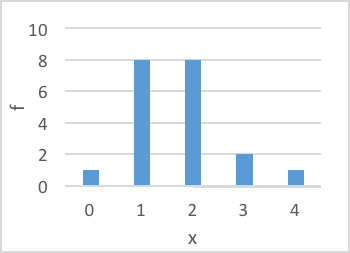
\includegraphics [width=0.4\textwidth ]{img-sol/t4-0}
	 \task* $P(5)=\frac {1}{6}$ i $P(Oros)=\frac {10}{40}$
\end{tasks}
 \end{enumerate}
\vspace{0.3cm}

 \needspace{4\baselineskip} 

{\textbf{\em Pàgina 45}} \hrulefill
\begin{enumerate}
\vspace{0.25cm}


 \needspace{2\baselineskip} 

 \item[\fontfamily{phv}\selectfont\color{blue}\textbf{1}. ] 
 \begin{tasks}[column-sep=1em, item-indent=1.3333em](1)
	 \task* La població són tots els alumnes de la classe
	 \task* La mostra són els 10 companys triats a l'atzar
	 \task* Qualssevol alumne de la classe que no hagués estat triat a l'atzar.
\end{tasks}
 \end{enumerate}
\begin{enumerate}
\vspace{0.25cm}


 \needspace{2\baselineskip} 

 \item[\fontfamily{phv}\selectfont\color{blue}\textbf{2}. ] 
 \begin{tasks}[column-sep=1em, item-indent=1.3333em](1)
	 \task Qualitativa
	 \task Quantitativa Discreta
	 \task Quantitativa Discreta
	 \task Quantitativa Contínua
	 \task Qualitativa
	 \task Quantitativa Discreta
	 \task Qualitativa
	 \task Quantitativa Contínua
	 \task Quantitativa Discreta
\end{tasks}
 \end{enumerate}
\vspace{0.3cm}

 \needspace{4\baselineskip} 

{\textbf{\em Pàgina 46}} \hrulefill
\begin{enumerate}
\vspace{0.25cm}


 \needspace{2\baselineskip} 

 \item[\fontfamily{phv}\selectfont\color{blue}\textbf{3}. ] 
 \begin{tasks}[column-sep=1em, item-indent=1.3333em](1)
	 \task Millor la mosta
	 \task Millor la població
\end{tasks}
 \end{enumerate}
\begin{enumerate}
\vspace{0.25cm}
\item[\fontfamily{phv}\selectfont\color{blue}\textbf{4. }] 
Segurament hauran utilitzat el programa Gestib que ho gestiona tot. En tal cas, estudien tota la població. Si l'estudi hagués comptat només amb les alumnes, el resultat no representaria a toda la població.
\vspace{0.25cm}
\item[\fontfamily{phv}\selectfont\color{blue}\textbf{5. }] 
Seria molt complicat consultar a tota la població (llarg i car). Millor una mostra.
\vspace{0.25cm}
\item[\fontfamily{phv}\selectfont\color{blue}\textbf{6. }] 
Solució oberta. Faríem un diagrama de sectors o de barres.
\vspace{0.25cm}
\item[\fontfamily{phv}\selectfont\color{blue}\textbf{7. }] 
 \begin {tabular}{c|c} Segons & f \\ \hline 10 & 3 \\ 11 & 4 \\ 12 & 3 \\ 13 & 3 \\ 14 & 0 \\ 15 & 4 \\ 16 & 3 \\ 18 & 3 \\ 19 & 2 \\ 20 & 2 \\ \end {tabular} \par 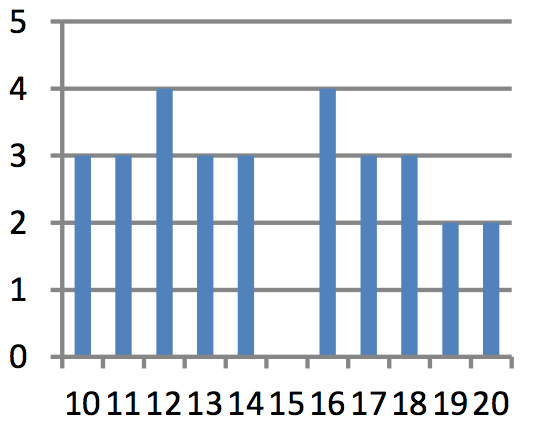
\includegraphics [width=0.35\textwidth ]{img-sol/t4-7} \par \ggblink {https://goo.gl/pWA3K9} 
 \end{enumerate}
\vspace{0.3cm}

 \needspace{4\baselineskip} 

{\textbf{\em Pàgina 48}} \hrulefill
\begin{enumerate}
\vspace{0.25cm}


 \needspace{2\baselineskip} 

 \item[\fontfamily{phv}\selectfont\color{blue}\textbf{8}. ]  \scalebox{0.6}{\simbolclau } 
 \begin{tasks}[column-sep=1em, item-indent=1.3333em](1)
	 \task* $\bar x=40.5$; $\sigma =16.5$; $CV=0.407$
	 \task* $\bar x=40.4$; $\sigma =17.11$; $CV=0.424$
	 \task* $\bar x=46.5$; $\sigma =9.74$; $CV=0.21$ \par \ggblink {https://goo.gl/JfqFSu}
\end{tasks}
 \end{enumerate}
\vspace{0.3cm}

 \needspace{4\baselineskip} 

{\textbf{\em Pàgina 49}} \hrulefill
\begin{enumerate}
\vspace{0.25cm}
\item[\fontfamily{phv}\selectfont\color{blue}\textbf{9. }]  \scalebox{0.6}{\simbolclau } 
$M_o =1$; $\bar x=1.6$; $Var=0.84$; $\sigma =0.92$\par \ggblink {https://goo.gl/nKce19}
 \end{enumerate}
\begin{enumerate}
\vspace{0.25cm}
\item[\fontfamily{phv}\selectfont\color{blue}\textbf{10. }]  \scalebox{0.6}{\simbolclau } 
Variable quantitativa discreta;\par $\bar x=1.6078$; $\sigma =0.9717$\par \ggblink {https://goo.gl/9tu6n7}
\vspace{0.25cm}
\item[\fontfamily{phv}\selectfont\color{blue}\textbf{11. }]  \scalebox{0.6}{\simbolclau } 
$\bar x=0.95$; $M_o=1$; $M_e$ = 1; $Q_1 = 1$; $Q_3= 1$ \par \ggblink {https://goo.gl/nFytiW} 
\vspace{0.25cm}
\item[\fontfamily{phv}\selectfont\color{blue}\textbf{12. }] 
Rang = 4. Desviació mitjana = 0,456. Variància = 0,299. Desviació típica = 0,5473; \par \ggblink {https://goo.gl/nFytiW}
\vspace{0.25cm}


 \needspace{2\baselineskip} 

 \item[\fontfamily{phv}\selectfont\color{blue}\textbf{13}. ] 
 \begin{tasks}[column-sep=1em, item-indent=1.3333em](2)
	 \task* Mitjana = 2.5; Mediana = 2; Moda = 2
	 \task* 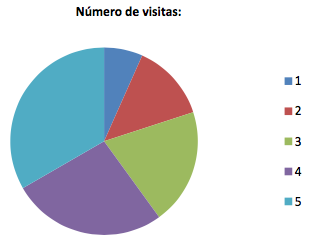
\includegraphics [width=0.35\textwidth ]{img-sol/t4-13}\par \ggblink {https://goo.gl/RtMKif}
\end{tasks}
 \end{enumerate}
\vspace{0.3cm}

 \needspace{4\baselineskip} 

{\textbf{\em Pàgina 50}} \hrulefill
\begin{enumerate}
\vspace{0.25cm}


 \needspace{2\baselineskip} 

 \item[\fontfamily{phv}\selectfont\color{blue}\textbf{14}. ] 
 \begin{tasks}[column-sep=1em, item-indent=1.3333em](2)
	 \task* $\bar x=93.8$; $\sigma =13.3$; $CV=0.142$
	 \task* 62.4 \% \par \ggblink {https://goo.gl/t62BLv}
\end{tasks}
 \end{enumerate}
\begin{enumerate}
\vspace{0.25cm}


 \needspace{2\baselineskip} 

 \item[\fontfamily{phv}\selectfont\color{blue}\textbf{15}. ] 
 \begin{tasks}[column-sep=1em, item-indent=1.3333em](2)
	 \task* 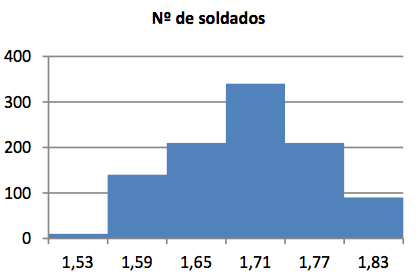
\includegraphics [width=0.35\textwidth ]{img-sol/t4-15}
	 \task* Mitjana = 1.7049. Desviació típica =0.07132
	 \task* Mediana. Per a calcular l'interval on es troba miram
	 \task* en la taula de les freqüències acumulades
	 \task* estan els 500 soldats. És l'interval 1,68 – 1,74.\par \ggblink {https://goo.gl/QVSssH} 
\end{tasks}
\vspace{0.25cm}
\item[\fontfamily{phv}\selectfont\color{blue}\textbf{16. }] 
Es pot representar mitjançant un diagrama de barres amb colors diferents per a cada any. La variable és quantitativa contínua i es poden calcular paràmetres estadístics. L'ordre dels països és Bèlgica$>$ Itàlia $>$ Grècia $>$ Espanya $>$ Alemanya $>$ França $>$ Portugal $>$ Regne Unit.\par \ggblink {https://goo.gl/Z6UoWb}
\vspace{0.25cm}
\item[\fontfamily{phv}\selectfont\color{blue}\textbf{17. }] 
 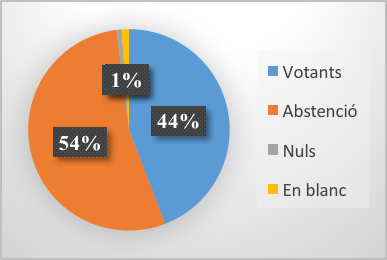
\includegraphics [width=0.4\textwidth ]{img-sol/t4-17} \par Cens=100 \%;\par Total de votants= 44,152 \%; \par Abstenció= 53,87 \%; \par Vots nuls= 0,82022727 \%; \par Vots en blanc= 1,1583\%; \par Ha guanyat l'abstenció, amb més de la meitat del cens.\par \ggblink {https://goo.gl/JjcnL4}
 \end{enumerate}
\vspace{0.3cm}

 \needspace{4\baselineskip} 

{\textbf{\em Pàgina 51}} \hrulefill
\begin{enumerate}
\vspace{0.25cm}


 \needspace{2\baselineskip} 

 \item[\fontfamily{phv}\selectfont\color{blue}\textbf{18}. ] 
 \begin{tasks}[column-sep=1em, item-indent=1.3333em](1)
	 \task Aleatori
	 \task Determinista
	 \task Determinista
	 \task Aleatori
	 \task Aleatori
\end{tasks}
 \end{enumerate}
\begin{enumerate}
\vspace{0.25cm}
\item[\fontfamily{phv}\selectfont\color{blue}\textbf{19. }] 
E=$\{VV, VN, NV, NN \}$
\vspace{0.25cm}
\item[\fontfamily{phv}\selectfont\color{blue}\textbf{20. }] 
\href {https://piworld.es/\#!/home/activity/71/0}{Simulació}:\par 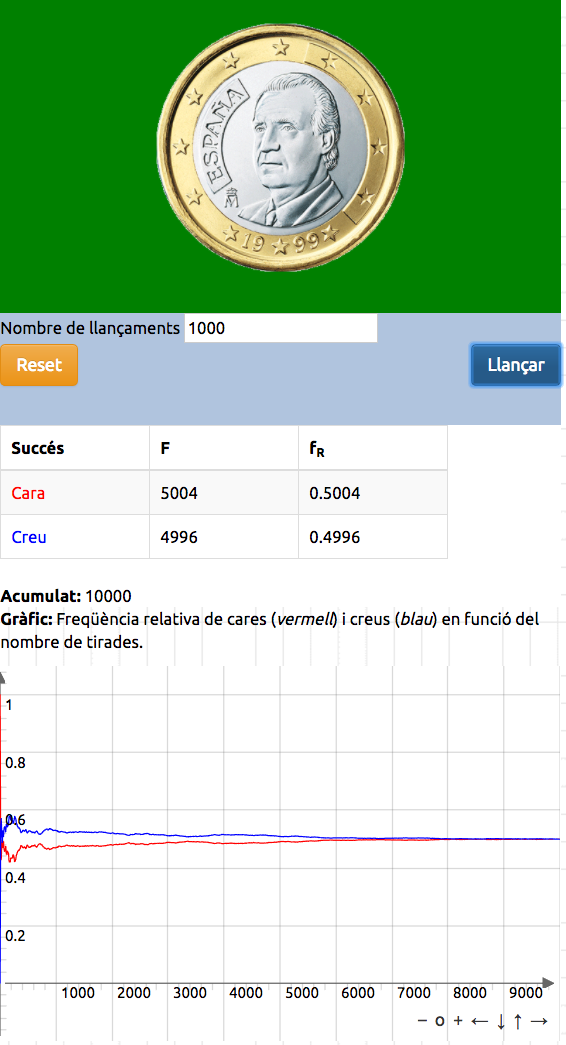
\includegraphics [width=0.4\textwidth ]{img-sol/t4-sim-monedes} \par \begin{tasks} \task Pel nombre més alt de tirades, cerca la freqüència relativa. Aquesta és la millor aproximació a la probabilitat d'obtenir cara. La probabilitat de treure creu és $P(X)=1-P(C)$ \task Sí. Són equiprobables. Perquè la moneda és simètrica i no està trucada.\end{tasks}
 \end{enumerate}
\vspace{0.3cm}

 \needspace{4\baselineskip} 

{\textbf{\em Pàgina 52}} \hrulefill
\begin{enumerate}
\vspace{0.25cm}


 \needspace{2\baselineskip} 

 \item[\fontfamily{phv}\selectfont\color{blue}\textbf{21}. ] 
 \begin{tasks}[column-sep=1em, item-indent=1.3333em](1)
	 \task Pel nombre més alt de tirades
	 \task* cerca la freqüència relativa. Aquesta és la millor aproximació a la probabilitat de caure per amunt. La probabilitat de caure de costat és $P(costat)=1-P(amunt)$
	 \task* No són equiprobables. Perquè la xinxeta pesa més d'una banda que de l'altre. Les dues bandes no són simètriques.
\end{tasks}
 \end{enumerate}
\begin{enumerate}
\vspace{0.25cm}
\item[\fontfamily{phv}\selectfont\color{blue}\textbf{22. }] 
L'experiment A és determinista perquè segur que surt bola vermella. L'experiment B és aleatori perquè no sabem el nombre que sortirà abans de fer l'experiment. L'espai mostral és E=\{1, 2, 3, 4, 5, 6, 7, 8, 9, 10\}
 \end{enumerate}
\vspace{0.3cm}

 \needspace{4\baselineskip} 

{\textbf{\em Pàgina 53}} \hrulefill
\begin{enumerate}
\vspace{0.25cm}


 \needspace{2\baselineskip} 

 \item[\fontfamily{phv}\selectfont\color{blue}\textbf{23}. ] 
 \begin{tasks}[column-sep=1em, item-indent=1.3333em](1)
	 \task $P(2)=\frac {1}{6}$; $P(5)=\frac {1}{6}$
	 \task $P(2)=\frac {1}{4}$; $P(5)=0$
	 \task $P(2)=\frac {1}{8}$; $P(5)=\frac {1}{8}$
\end{tasks}
 \end{enumerate}
\begin{enumerate}
\vspace{0.25cm}


 \needspace{2\baselineskip} 

 \item[\fontfamily{phv}\selectfont\color{blue}\textbf{24}. ] 
 \begin{tasks}[column-sep=1em, item-indent=1.3333em](2)
	 \task $\frac {4}{20}$
	 \task $\frac {19}{20}$
	 \task $\frac {13}{20}$
	 \task $\frac {11}{20}$
\end{tasks}
\vspace{0.25cm}
\item[\fontfamily{phv}\selectfont\color{blue}\textbf{25. }] 
De la bossa I. Perquè P(I)=$\frac {2}{3}=0.666...$, P(II)=$\frac {4}{7}=0.571$ i P(III)=$\frac {3}{5}=0.6$
\vspace{0.25cm}


 \needspace{2\baselineskip} 

 \item[\fontfamily{phv}\selectfont\color{blue}\textbf{26}. ] 
 \begin{tasks}[column-sep=1em, item-indent=1.3333em](2)
	 \task $\frac {2}{6}$
	 \task $\frac {3}{6}$
	 \task $\frac {5}{6}$
	 \task $\frac {4}{6}$
	 \task 0
	 \task $\frac {3}{6}$
\end{tasks}
\vspace{0.25cm}


 \needspace{2\baselineskip} 

 \item[\fontfamily{phv}\selectfont\color{blue}\textbf{27}. ] 
 \begin{tasks}[column-sep=1em, item-indent=1.3333em](2)
	 \task $\frac {10}{40}$
	 \task $\frac {24}{40}$
	 \task $\frac {20}{40}$
	 \task $\frac {19}{40}$
\end{tasks}
\vspace{0.25cm}


 \needspace{2\baselineskip} 

 \item[\fontfamily{phv}\selectfont\color{blue}\textbf{28}. ] 
 \begin{tasks}[column-sep=1em, item-indent=1.3333em](2)
	 \task $\frac {4}{40}$
	 \task $\frac {36}{40}$
	 \task $\frac {20}{40}$
	 \task $\frac {30}{40}$
\end{tasks}
 \end{enumerate}
\vspace{0.3cm}

 \needspace{4\baselineskip} 

{\textbf{\em Pàgina 54}} \hrulefill
\begin{enumerate}
\vspace{0.25cm}


 \needspace{2\baselineskip} 

 \item[\fontfamily{phv}\selectfont\color{blue}\textbf{29}. ]  \scalebox{0.6}{\simbolclau } 
 \begin{tasks}[column-sep=1em, item-indent=1.3333em](3)
	 \task $\dfrac {58}{120}$
	 \task $\dfrac {16}{120}$
	 \task* $\dfrac {62}{120}$ i $\dfrac {1}{120}$ 
\end{tasks}
 \end{enumerate}
\begin{enumerate}
\vspace{0.25cm}


 \needspace{2\baselineskip} 

 \item[\fontfamily{phv}\selectfont\color{blue}\textbf{30}. ] 
 \begin{tasks}[column-sep=1em, item-indent=1.3333em](2)
	 \task $\frac {1}{10}$
	 \task $\frac {1}{10}$
	 \task $\frac {7}{10}$
	 \task $\frac {3}{10}$
\end{tasks}
\vspace{0.25cm}


 \needspace{2\baselineskip} 

 \item[\fontfamily{phv}\selectfont\color{blue}\textbf{31}. ] 
 \begin{tasks}[column-sep=1em, item-indent=1.3333em](2)
	 \task $\frac {7}{29}\approx 0.24$
	 \task $\frac {18}{29}\approx 0.62$
\end{tasks}
 \end{enumerate}
\vspace{0.3cm}

 \needspace{4\baselineskip} 

{\textbf{\em Pàgina 55}} \hrulefill
\begin{enumerate}
\vspace{0.25cm}


 \needspace{2\baselineskip} 

 \item[\fontfamily{phv}\selectfont\color{blue}\textbf{32}. ] 
 \begin{tasks}[column-sep=1em, item-indent=1.3333em](2)
	 \task* $\frac {1}{6}\cdot \frac {1}{2}=\frac {1}{12}$
	 \task* $\frac {3}{6}\cdot \frac {1}{2}=\frac {1}{4}$
\end{tasks}
 \end{enumerate}
\begin{enumerate}
\vspace{0.25cm}
\item[\fontfamily{phv}\selectfont\color{blue}\textbf{33. }] 
Si $A$=\{1,2,3,4,5,6\}, cal calcular el producte cartesià $A\times A$.\par \begin{tasks}(2) \task $\frac {11}{36}$ \task $\frac {5}{36}$ \task $\frac {25}{36}$ \task $\frac {31}{36}$\end{tasks}
\vspace{0.25cm}


 \needspace{2\baselineskip} 

 \item[\fontfamily{phv}\selectfont\color{blue}\textbf{34}. ]  \scalebox{0.6}{\simbolclau } 
 \begin{tasks}[column-sep=1em, item-indent=1.3333em](2)
	 \task $\frac {1}{2}$
	 \task $\frac {1}{2}$
	 \task $\frac {1}{2}$
	 \task $1-\dfrac {1}{8}=\dfrac {7}{8}$
	 \task $\frac {1}{8}$
	 \task $\frac {1}{8}$
\end{tasks}
\vspace{0.25cm}


 \needspace{2\baselineskip} 

 \item[\fontfamily{phv}\selectfont\color{blue}\textbf{35}. ]  \scalebox{0.6}{\simbolclau } 
 \begin{tasks}[column-sep=1em, item-indent=1.3333em](3)
	 \task 0.19
	 \task 0.44
	 \task 0.56
	 \task 0.95
	 \task 0.65
	 \task 0.35
\end{tasks}
 \end{enumerate}
\vspace{0.3cm}

 \needspace{4\baselineskip} 

{\textbf{\em Pàgina 56}} \hrulefill
\begin{enumerate}
\vspace{0.25cm}


 \needspace{2\baselineskip} 

 \item[\fontfamily{phv}\selectfont\color{blue}\textbf{36}. ] 
 \begin{tasks}[column-sep=1em, item-indent=1.3333em](1)
	 \task* $\left (\frac {1}{2}\right )^4= \frac {1}{16}$
	 \task* $1-P(CCCC)=1-\frac {1}{16}=\frac {15}{16}$
	 \task* $4 P(XCCC)=4\left (\frac {1}{2}\right )^4=\frac {1}{4}$
\end{tasks}
 \end{enumerate}
\begin{enumerate}
\vspace{0.25cm}


 \needspace{2\baselineskip} 

 \item[\fontfamily{phv}\selectfont\color{blue}\textbf{37}. ]  \scalebox{0.6}{\simbolclau } 
 \begin{tasks}[column-sep=1em, item-indent=1.3333em](3)
	 \task $\dfrac {49}{100}$
	 \task $\dfrac {91}{100}$
	 \task $\dfrac {9}{100}$
\end{tasks}
\vspace{0.25cm}


 \needspace{2\baselineskip} 

 \item[\fontfamily{phv}\selectfont\color{blue}\textbf{38}. ]  \scalebox{0.6}{\simbolclau } 
 \begin{tasks}[column-sep=1em, item-indent=1.3333em](3)
	 \task $\dfrac {91}{100}$
	 \task $\dfrac {35}{38}$
	 \task $\dfrac {3}{38}$
\end{tasks}
\vspace{0.25cm}


 \needspace{2\baselineskip} 

 \item[\fontfamily{phv}\selectfont\color{blue}\textbf{39}. ] 
 \begin{tasks}[column-sep=1em, item-indent=1.3333em](1)
	 \task* Amb reemplaçament $P(RRR)=\frac {4}{40}\cdot \frac {4}{40} \cdot \frac {4}{40} =\frac {1}{1000}=0.001$
	 \task* Sense reemplaçament $P(RRR)=\frac {4}{40}\cdot \frac {3}{39} \cdot \frac {2}{38} =\frac {1}{2470}=0.0004$
\end{tasks}
 \end{enumerate}
\vspace{0.3cm}

 \needspace{4\baselineskip} 

{\textbf{\em Pàgina 57}} \hrulefill
\begin{enumerate}
\vspace{0.25cm}


 \needspace{2\baselineskip} 

 \item[\fontfamily{phv}\selectfont\color{blue}\textbf{40}. ] 
 \begin{tasks}[column-sep=1em, item-indent=1.3333em](1)
	 \task $P(CC)=\frac {1}{4}$
	 \task $P(XCC)=\frac {1}{8}$
\end{tasks}
 \end{enumerate}
\begin{enumerate}
\vspace{0.25cm}
\item[\fontfamily{phv}\selectfont\color{blue}\textbf{41. }]  \scalebox{0.6}{\simbolclau } 
$P=0.9999$
\vspace{0.25cm}
\item[\fontfamily{phv}\selectfont\color{blue}\textbf{42. }] 
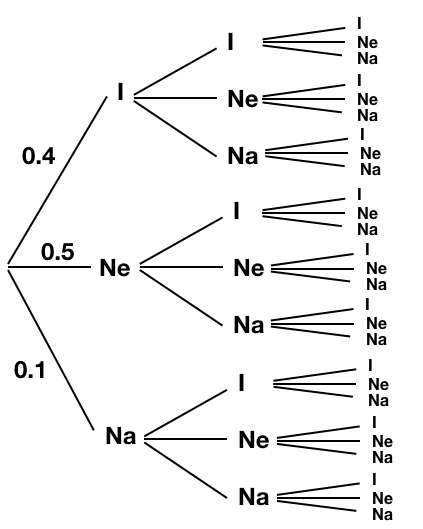
\includegraphics [width=0.35\textwidth ]{img-sol/t4-42} \par \begin{tasks} \task $P=1 – P(cap intencionat) = 1 – 0.63 = 0.784$ \task $P=(0.1)^3=0.001$, $P=0.5^3=0.125$ \end{tasks}
\vspace{0.25cm}
\item[\fontfamily{phv}\selectfont\color{blue}\textbf{43. }] 
Fer el producte cartesià.\par S'obté $P=\frac {12}{36}=\frac {1}{3}$
\vspace{0.25cm}
\item[\fontfamily{phv}\selectfont\color{blue}\textbf{44. }] 
\begin {tabular}{c|ccc} & As & No As & \\ \hline Copa & 0.04 & 0.04 & 0.08 \\ No copa & 0.08 & 0.84 & 0.92 \\ & 0.12 & 0.88 & 1 \\ \end {tabular} \par P(As copes)=0.04; No s'ha eliminat l'as de copes.
\vspace{0.25cm}


 \needspace{2\baselineskip} 

 \item[\fontfamily{phv}\selectfont\color{blue}\textbf{45}. ]  \scalebox{0.6}{\simbolclau } 
 \begin{tasks}[column-sep=1em, item-indent=1.3333em](2)
	 \task $\dfrac {28}{153}$
	 \task $\dfrac {49}{153}$
	 \task $\dfrac {62}{153}$
	 \task $\dfrac {80}{153}$
\end{tasks}
\vspace{0.25cm}


 \needspace{2\baselineskip} 

 \item[\fontfamily{phv}\selectfont\color{blue}\textbf{46}. ] 
 \begin{tasks}[column-sep=1em, item-indent=1.3333em](1)
	 \task* $3\left (\dfrac {1}{365}\right )\left (\dfrac {364}{365}\right )^2 = 0,008174203184$
	 \task* $3 \left (\dfrac {1}{365}\right )^2 \left (\dfrac {364}{365}\right )+ \left (\dfrac {1}{365}\right )^3 = 0,000022456602$ 
\end{tasks}
 \end{enumerate}
\vspace{0.3cm}

 \needspace{4\baselineskip} 

{\textbf{\em Pàgina 58}} \hrulefill
\begin{enumerate}
\vspace{0.25cm}
 \item[$\bullet$ ] {\fontfamily{phv}\selectfont\color{blue}\textbf{Autoavaluació:}. }

 \end{enumerate}
\begin{enumerate}
\vspace{0.25cm}
\item[\fontfamily{phv}\selectfont\color{blue}\textbf{1. }]  \scalebox{0.6}{\simbolclau } 
\textbf {--10.}: Claus de l'autoavaluació: 1b; 2c; 3c; 4b; 5d; 6a; 7a; 8b; 9d; 10c
 \end{enumerate}
\vfill\null
\columnbreak
\def\currentname{Solucions del Tema 5}
\vspace*{0.75cm}

 
 \needspace{5\baselineskip} 
 \scalebox{1.25}{\heading{Solucions del Tema 5}}

\vspace*{0.4cm}
\phantomsection \addcontentsline{toc}{section}{Solucions del Tema 5}
\vspace{0.3cm}

 \needspace{4\baselineskip} 

{\textbf{\em Pàgina 60}} \hrulefill
\begin{enumerate}
\vspace{0.25cm}
 \item[$\bullet$ ] {\fontfamily{phv}\selectfont\color{blue}\textbf{Avaluació inicial}. }
N'hi ha 8 de falses:\par $a+a=a^2$,\par $3a\cdot 4b=7ab$,\par $3b-2=b$,\par $a+b=ab$,\par $2a+b=2ab$,\par $3b-3b=b$,\par $3a\cdot a=6a$,\par $2a+1=3a$
 \end{enumerate}
\vspace{0.3cm}

 \needspace{4\baselineskip} 

{\textbf{\em Pàgina 61}} \hrulefill
\begin{enumerate}
\vspace{0.25cm}
\item[\fontfamily{phv}\selectfont\color{blue}\textbf{1. }] 
l'àrea d'un quadrat = $x^2$ i la longitud d'una circumferència = $2\pi r$. Són monomis de grau 2 i 1 respectivament.
 \end{enumerate}
\begin{enumerate}
\vspace{0.25cm}


 \needspace{2\baselineskip} 

 \item[\fontfamily{phv}\selectfont\color{blue}\textbf{2}. ] 
 \begin{tasks}[column-sep=1em, item-indent=1.3333em](2)
	 \task $3(x-y)$
	 \task $x^2+y^2$
	 \task $(x+y)^2$
	 \task $\frac {1}{x\cdot y}$
	 \task $-x+(-y)$
	 \task $x^2\cdot y^2$
\end{tasks}
\vspace{0.25cm}
\item[\fontfamily{phv}\selectfont\color{blue}\textbf{3. }] 
L'import de la factura és $0,12 \cdot N + 0,05\cdot M$ euros.
\vspace{0.25cm}
\item[\fontfamily{phv}\selectfont\color{blue}\textbf{4. }] 
Pagarem el 70\% de $x=0.7 x$
 \end{enumerate}
\vspace{0.3cm}

 \needspace{4\baselineskip} 

{\textbf{\em Pàgina 62}} \hrulefill
\begin{enumerate}
\vspace{0.25cm}


 \needspace{2\baselineskip} 

 \item[\fontfamily{phv}\selectfont\color{blue}\textbf{5}. ] 
 \begin{tasks}[column-sep=1em, item-indent=1.3333em](3)
	 \task $0$
	 \task $-1$
	 \task $-2$
\end{tasks}
 \end{enumerate}
\begin{enumerate}
\vspace{0.25cm}


 \needspace{2\baselineskip} 

 \item[\fontfamily{phv}\selectfont\color{blue}\textbf{6}. ] 
 \begin{tasks}[column-sep=1em, item-indent=1.3333em](3)
	 \task $1$
	 \task $-1$
	 \task $11$
\end{tasks}
\vspace{0.25cm}


 \needspace{2\baselineskip} 

 \item[\fontfamily{phv}\selectfont\color{blue}\textbf{7}. ] 
 \begin{tasks}[column-sep=1em, item-indent=1.3333em](2)
	 \task $\frac {9}{4}$
	 \task $9$
\end{tasks}
\vspace{0.25cm}
\item[\fontfamily{phv}\selectfont\color{blue}\textbf{8. }] 
L'expressió simplificada de la suma és $4(x+y)-x^2-y^2$ i presenta un màxim a $x=y=2$. El valor màxim d'aquesta suma és 8.
 \end{enumerate}
\vspace{0.3cm}

 \needspace{4\baselineskip} 

{\textbf{\em Pàgina 63}} \hrulefill
\begin{enumerate}
\vspace{0.25cm}
\item[\fontfamily{phv}\selectfont\color{blue}\textbf{9. }] 
 \begin {tabular}{|c|c|c|c|} \hline \rowcolor {lightgray} Monomi & Coef & P.literal & Grau \\ \hline $-12x^{3} $ & -12 & $x^3$ & 3 \\ \hline $a^{4} b^{3} c$ & 1 & $a^{4} b^{3} c$ & 8 \\ \hline $4xy^{2} $ & 4 & $xy^2$ & 3 \\ \hline \end {tabular} 
 \end{enumerate}
\begin{enumerate}
\vspace{0.25cm}


 \needspace{2\baselineskip} 

 \item[\fontfamily{phv}\selectfont\color{blue}\textbf{10}. ] 
 \begin{tasks}[column-sep=1em, item-indent=1.3333em](2)
	 \task $8x$
	 \task $25y$
	 \task $-6ab$
	 \task $10x^5$
	 \task $\frac {9}{2}z^2$
	 \task $-\frac {3}{4}x^2$
	 \task $\frac {11}{6}x^4y^3$
	 \task $5a$
\end{tasks}
\vspace{0.25cm}


 \needspace{2\baselineskip} 

 \item[\fontfamily{phv}\selectfont\color{blue}\textbf{11}. ] 
 \begin{tasks}[column-sep=1em, item-indent=1.3333em](2)
	 \task $2x^4$
	 \task $8x^{12}$
	 \task $\frac {2}{15}y^6$
	 \task $-x^2$
	 \task $-\frac {1}{2}x^{12}$
	 \task $6x^2 y$
	 \task $15x^3 y^6$
	 \task $a^3 b^3$
\end{tasks}
 \end{enumerate}
\vspace{0.3cm}

 \needspace{4\baselineskip} 

{\textbf{\em Pàgina 64}} \hrulefill
\begin{enumerate}
\vspace{0.25cm}


 \needspace{2\baselineskip} 

 \item[\fontfamily{phv}\selectfont\color{blue}\textbf{12}. ] 
 \begin{tasks}[column-sep=1em, item-indent=1.3333em](2)
	 \task $x$
	 \task $\frac {x}{2}$
	 \task $3x^3$
	 \task $4x^2$
	 \task $\frac {1}{2}$
	 \task $\frac {3}{2}x^5$
	 \task $-3x^2$
	 \task $-3x^3$
	 \task $-3$
	 \task $-10xy$
	 \task $-3x^3$
	 \task $-\frac {5}{2}a b^2$
\end{tasks}
 \end{enumerate}
\begin{enumerate}
\vspace{0.25cm}


 \needspace{2\baselineskip} 

 \item[\fontfamily{phv}\selectfont\color{blue}\textbf{13}. ] 
 \begin{tasks}[column-sep=1em, item-indent=1.3333em](2)
	 \task $2x^2$
	 \task $-5x^2$
	 \task $4x^2 y$
	 \task $\frac {5}{3} x y^2$
	 \task $6x ^2$
	 \task $4 a^2 b^2$
	 \task $-7b$
	 \task $\frac {29}{9}x$
\end{tasks}
 \end{enumerate}
\vspace{0.3cm}

 \needspace{4\baselineskip} 

{\textbf{\em Pàgina 65}} \hrulefill
\begin{enumerate}
\vspace{0.25cm}
\item[\fontfamily{phv}\selectfont\color{blue}\textbf{14. }] 
\par \begin {tabular}{|c|c|c|c|} \hline \rowcolor {lightgray} Poli. & Termes & Grau & T.I. \\ \hline $5x^{4} +7x^{2}$ & 2 & 4 & 0 \\ \hline $6x^{2} +10-2x^{3} $ & 3 & 3 & 10 \\ \hline $3x^{4}-5x^{3}+x^2+1 $ & 4 & 4 & 1 \\ \hline $2xy^{3} -x^{5} +7x^{2} y^{2}$ & 4 & 5 & 0 \\ \hline \end {tabular}
 \end{enumerate}
\begin{enumerate}
\vspace{0.25cm}


 \needspace{2\baselineskip} 

 \item[\fontfamily{phv}\selectfont\color{blue}\textbf{15}. ] 
 \begin{tasks}[column-sep=1em, item-indent=1.3333em](2)
	 \task $2$
	 \task $0$
	 \task $4$
	 \task $0$
	 \task $\frac {5}{8}$
\end{tasks}
\vspace{0.25cm}


 \needspace{2\baselineskip} 

 \item[\fontfamily{phv}\selectfont\color{blue}\textbf{16}. ] 
 \begin{tasks}[column-sep=1em, item-indent=1.3333em](1)
	 \task $-5x^3+9x-1$
	 \task $-6x^3+3x^2-x+9$
\end{tasks}
\vspace{0.25cm}


 \needspace{2\baselineskip} 

 \item[\fontfamily{phv}\selectfont\color{blue}\textbf{17}. ] 
 \begin{tasks}[column-sep=1em, item-indent=1.3333em](1)
	 \task $5x^2+2x+2$
	 \task $-2x^3+6x+1$
	 \task $-3x^3+3x^2-x-1$
\end{tasks}
\vspace{0.25cm}
\item[\fontfamily{phv}\selectfont\color{blue}\textbf{18. }] 
El polinomi suma $S(x)=-x^3+x^2+x-2$; els valors numèrics $P(-2)=7$, $Q(-2)=1$ i $S(-2)=8$. Es compleix que $S(-2)=P(-2)+Q(-2)$. 
\vspace{0.25cm}


 \needspace{2\baselineskip} 

 \item[\fontfamily{phv}\selectfont\color{blue}\textbf{19}. ] 
 \begin{tasks}[column-sep=1em, item-indent=1.3333em](1)
	 \task $x^3+3x^2-x$
	 \task $-6x^2+15x$
	 \task $-6x^7+8x^4-16x^3$
	 \task $9x^7+3x^3$
\end{tasks}
 \end{enumerate}
\vspace{0.3cm}

 \needspace{4\baselineskip} 

{\textbf{\em Pàgina 66}} \hrulefill
\begin{enumerate}
\vspace{0.25cm}


 \needspace{2\baselineskip} 

 \item[\fontfamily{phv}\selectfont\color{blue}\textbf{20}. ] 
 \begin{tasks}[column-sep=1em, item-indent=1.3333em](1)
	 \task $2(x^2+x+1)$
	 \task $x(x+1)$
	 \task $5x(3x+1)$
	 \task $-4(4x^2+x+2)$
	 \task $-5x(2x^2+3x-4)$
	 \task $6x^2(5x^2+6)$
\end{tasks}
 \end{enumerate}
\begin{enumerate}
\vspace{0.25cm}


 \needspace{2\baselineskip} 

 \item[\fontfamily{phv}\selectfont\color{blue}\textbf{21}. ] 
 \begin{tasks}[column-sep=1em, item-indent=1.3333em](1)
	 \task $-6x^3+8x$
	 \task $-8x^4+10x^3-4x+5$
	 \task $8x^4+22x^3-6x^2-2x-6$
	 \task $-8x^2-7x+9$
\end{tasks}
\vspace{0.25cm}


 \needspace{2\baselineskip} 

 \item[\fontfamily{phv}\selectfont\color{blue}\textbf{22}. ] 
 \begin{tasks}[column-sep=1em, item-indent=1.3333em](1)
	 \task $-2x^2+4x$
	 \task $6x^2-5x-6$
	 \task $-3a^2+10a-8$
	 \task $-3a^3 + a^2b^2+6ab-2b^3$
\end{tasks}
\vspace{0.25cm}


 \needspace{2\baselineskip} 

 \item[\fontfamily{phv}\selectfont\color{blue}\textbf{23}. ]  \scalebox{0.6}{\simbolclau } 
 \begin{tasks}[column-sep=1em, item-indent=1.3333em](1)
	 \task $-3x^5+4x^4+2x^3$
	 \task $10x^4-8x^3+7x^2-3x$
	 \task $12\,a^3-43\,a^2+43\,a-10$
\end{tasks}
 \end{enumerate}
\vspace{0.3cm}

 \needspace{4\baselineskip} 

{\textbf{\em Pàgina 67}} \hrulefill
\begin{enumerate}
\vspace{0.25cm}


 \needspace{2\baselineskip} 

 \item[\fontfamily{phv}\selectfont\color{blue}\textbf{24}. ]  \scalebox{0.6}{\simbolclau } 
 \begin{tasks}[column-sep=1em, item-indent=1.3333em](1)
	 \task $Q=3x-2$; $R=-2x+5$
	 \task $Q=-2$; $R=4x^2-x+6$
	 \task $Q=2x^2+3x$; $R=-16x+7$
	 \task $Q=3x^2-3x+4$; $R=-x+2$
	 \task $Q=x^3-3x$; $R=5x-6$
\end{tasks}
 \end{enumerate}
\begin{enumerate}
\vspace{0.25cm}


 \needspace{2\baselineskip} 

 \item[\fontfamily{phv}\selectfont\color{blue}\textbf{25}. ]  \scalebox{0.6}{\simbolclau } 
 \begin{tasks}[column-sep=1em, item-indent=1.3333em](1)
	 \task $Q=3x-11$; $R=38$
	 \task $Q=x^3+2x^2+4x+8$; $R=0$
	 \task $Q=x^3+x$; $R=1$
	 \task* $Q=7x^4-14x^3+24x^2-48x+103$; $R=-211$
\end{tasks}
\vspace{0.25cm}


 \needspace{2\baselineskip} 

 \item[\fontfamily{phv}\selectfont\color{blue}\textbf{26}. ] 
 \begin{tasks}[column-sep=1em, item-indent=1.3333em](1)
	 \task $Q=2x^2-5x+3$; $R=-2$
	 \task* $Q=-4x^4+8x^3+7x^2-21x+8$; $R=2x^2-3x+1$
	 \task $Q=3x^2-4$; $R=-2x-2$
\end{tasks}
 \end{enumerate}
\vspace{0.3cm}

 \needspace{4\baselineskip} 

{\textbf{\em Pàgina 68}} \hrulefill
\begin{enumerate}
\vspace{0.25cm}
\item[\fontfamily{phv}\selectfont\color{blue}\textbf{27. }] 
Hi ha infinites solucions. Per exemple, si ens inventam el divisor=$2x+3$, el dividend=quocient·divisor + residu = $(x^2-2x-1)(2x+3)+2x^2-3=2x^3+x^2-8x-6$
 \end{enumerate}
\begin{enumerate}
\vspace{0.25cm}


 \needspace{2\baselineskip} 

 \item[\fontfamily{phv}\selectfont\color{blue}\textbf{28}. ] 
 \begin{tasks}[column-sep=1em, item-indent=1.3333em](1)
	 \task $1+2x+x^2$
	 \task $x^2-4x+4$
	 \task $x^2-4x+4$
	 \task $4a^2-12a+9$
	 \task Atenció 3: $x^6+3x^4+3x^2+1$
	 \task Atenció 3: $8b^3-48b^2+96b-64$
\end{tasks}
\vspace{0.25cm}


 \needspace{2\baselineskip} 

 \item[\fontfamily{phv}\selectfont\color{blue}\textbf{29}. ] 
 \begin{tasks}[column-sep=1em, item-indent=1.3333em](2)
	 \task $9x^2-4$
	 \task $4x^2-16y^2$
	 \task $16x^4-9$
	 \task $9a^2-25b^2$
	 \task $x^6-16$
	 \task $-x^4+25x^2$
\end{tasks}
\vspace{0.25cm}


 \needspace{2\baselineskip} 

 \item[\fontfamily{phv}\selectfont\color{blue}\textbf{30}. ] 
 \begin{tasks}[column-sep=1em, item-indent=1.3333em](2)
	 \task $9x^2-6xy+y^2$
	 \task $4a^2+2ax+\frac {x^2}{4}$
	 \task $16y^2-16+\frac {4}{y^2}$
	 \task $25a^2+10a^3+a^4$
	 \task $a^4-4a^2b^2+4b^4$
	 \task* $\frac {4y^2}{9}-\frac {4}{3}+\frac {1}{y^2}$
\end{tasks}
 \end{enumerate}
\vspace{0.3cm}

 \needspace{4\baselineskip} 

{\textbf{\em Pàgina 69}} \hrulefill
\begin{enumerate}
\vspace{0.25cm}


 \needspace{2\baselineskip} 

 \item[\fontfamily{phv}\selectfont\color{blue}\textbf{31}. ] 
 \begin{tasks}[column-sep=1em, item-indent=1.3333em](2)
	 \task $(a-3)^2$
	 \task $(2x+1)^2$
	 \task $(b-5)^2$
	 \task $(2y-3)^2$
	 \task $(a^2+1)^2$
	 \task $(y^2+3x)^2$
\end{tasks}
 \end{enumerate}
\begin{enumerate}
\vspace{0.25cm}


 \needspace{2\baselineskip} 

 \item[\fontfamily{phv}\selectfont\color{blue}\textbf{32}. ] 
 \begin{tasks}[column-sep=1em, item-indent=1.3333em](1)
	 \task $(3x+5)(3x-5)$
	 \task $(2a^2+9b)(2a^2-9b)$
	 \task $(7+5x)(7-5x)$
	 \task $(10a+8)(10a-8)$
\end{tasks}
\vspace{0.25cm}


 \needspace{2\baselineskip} 

 \item[\fontfamily{phv}\selectfont\color{blue}\textbf{33}. ] 
 \begin{tasks}[column-sep=1em, item-indent=1.3333em](1)
	 \task $(x+6)^2 / (x+6)=x+6$
	 \task* $(2x^2+4x)(2x^2-4x)/(2x^2-4x)=2x^2+4x$
	 \task $(3x-4)^2/(3x-4)=3x-4$
	 \task $(x+2)(x-2)/(x+2)=x-2$
\end{tasks}
\vspace{0.25cm}


 \needspace{2\baselineskip} 

 \item[\fontfamily{phv}\selectfont\color{blue}\textbf{34}. ] 
 \begin{tasks}[column-sep=1em, item-indent=1.3333em](1)
	 \task $a^2+b^2+c^2+2ab+2ac+2bc$
	 \task $a^2+b^2+c^2-2ab+2ac-2bc$
\end{tasks}
 \end{enumerate}
\vspace{0.3cm}

 \needspace{4\baselineskip} 

{\textbf{\em Pàgina 70}} \hrulefill
\begin{enumerate}
\vspace{0.25cm}


 \needspace{2\baselineskip} 

 \item[\fontfamily{phv}\selectfont\color{blue}\textbf{35}. ]  \scalebox{0.6}{\simbolclau } 
 \begin{tasks}[column-sep=1em, item-indent=1.3333em](2)
	 \task $\frac {3x+3}{x^2+x-2}$
	 \task $\frac {-4x+3}{x^2-x}$
	 \task $\frac {-3x^3+3x^2}{x^2+4x+3}$
	 \task $\frac {x^2-x-6}{x^3}$
\end{tasks}
 \end{enumerate}
\begin{enumerate}
\vspace{0.25cm}


 \needspace{2\baselineskip} 

 \item[\fontfamily{phv}\selectfont\color{blue}\textbf{36}. ]  \scalebox{0.6}{\simbolclau } 
 \begin{tasks}[column-sep=1em, item-indent=1.3333em](2)
	 \task $\frac {x^2+1}{x^3}$
	 \task $\frac {-x-1}{x^2-2x}$
\end{tasks}
\vspace{0.25cm}


 \needspace{2\baselineskip} 

 \item[\fontfamily{phv}\selectfont\color{blue}\textbf{37}. ] 
 \begin{tasks}[column-sep=1em, item-indent=1.3333em](2)
	 \task $x^2-4x+3$
	 \task $a^3+12a^2-4$
	 \task $2x+5$
	 \task $6xy-4$
\end{tasks}
\vspace{0.25cm}


 \needspace{2\baselineskip} 

 \item[\fontfamily{phv}\selectfont\color{blue}\textbf{39}. ] 
 \begin{tasks}[column-sep=1em, item-indent=1.3333em](1)
	 \task* $\frac {3x(x+2)}{3(3x^2+6)}=\frac {x(x+2)}{3x^2+6}$
	 \task* $\frac {a^2(a-7)}{a^2(3a+5)}=\frac {a-7}{3a+5}$
	 \task* $\frac {ay(xy-7y)}{2xy}=\frac {y(x-7)}{2}$
	 \task* $\frac {ab(ab-1)}{ab(a^2+1)}=\frac {ab-1}{a^2-1}$
\end{tasks}
\vspace{0.25cm}


 \needspace{2\baselineskip} 

 \item[\fontfamily{phv}\selectfont\color{blue}\textbf{40}. ]  \scalebox{0.6}{\simbolclau } 
 \begin{tasks}[column-sep=1em, item-indent=1.3333em](2)
	 \task $\frac {x-2}{3}$
	 \task $\frac {2(x-4)}{x+4}$
	 \task $\frac {-2}{2a+3}$
	 \task $\frac {x}{x-2}$
\end{tasks}
 \end{enumerate}
\vspace{0.3cm}

 \needspace{4\baselineskip} 

{\textbf{\em Pàgina 71}} \hrulefill
\begin{enumerate}
\vspace{0.25cm}
\item[\fontfamily{phv}\selectfont\color{blue}\textbf{41. }] 
 Anomenarem $n$ al nombre de viatgers, $p$ al preu per viatger i $T$ a la quantitat total ingressada per l'empresa.\par Tots els valors de les variables són nombres enters.\par Si $n <101$: $P = 150$; $T = 150N$\par Si $n = 100 + x (0 <x <61)$: $p = 150 - x$; $T = 15 000 + 50x - x^2$\par Si $n> 160$: $p = 90$; $T = 90N.$
 \end{enumerate}
\begin{enumerate}
\vspace{0.25cm}
\item[\fontfamily{phv}\selectfont\color{blue}\textbf{42. }] 
 Si anomenam $2n$ al nombre parell inicial, la seqüència d'operacions dóna lloc a $\frac {[(10n+5)\cdot 2 -10]\cdot 5}{100}-n = 0$. 
\vspace{0.25cm}
\item[\fontfamily{phv}\selectfont\color{blue}\textbf{43. }] 
 Si anomenem $s$ al salari de 2014, els salaris dels anys successius són:\par $0,9 s$; $0,99 s$; $0,891 s$; $0,9801 s$; $0,88209 s$; $0,970299 s$; ... Els salaris són cada vegada menors que dos anys abans.
\vspace{0.25cm}


 \needspace{2\baselineskip} 

 \item[\fontfamily{phv}\selectfont\color{blue}\textbf{44}. ] 
 \begin{tasks}[column-sep=1em, item-indent=1.3333em](1)
	 \task Per a $x=-1$
	 \task Per a $x=5$ ni $x=-7/2$
	 \task Per a $x=1$
	 \task Es pot avaluar per tot $x$; $y$
\end{tasks}
\vspace{0.25cm}
\item[\fontfamily{phv}\selectfont\color{blue}\textbf{45. }] 
Per exemple: $(x+2)^2 + 6 = x^2 + 4x + 10$
\vspace{0.25cm}
\item[\fontfamily{phv}\selectfont\color{blue}\textbf{46. }] 
 $p+q+r=-x^4-x^3+2\,x^2-4$, \par $p-q=x^4+5\,x^3-3\,x^2+5\,x+4$, \par $p\cdot r=2\,x^5-7\,x^4+11\,x^3-15\,x^2+11\,x-2$, \par $p\cdot r-q=2\,x^5-6\,x^4+14\,x^3-17\,x^2+12\,x+3$
 \end{enumerate}
\vspace{0.3cm}

 \needspace{4\baselineskip} 

{\textbf{\em Pàgina 72}} \hrulefill
\begin{enumerate}
\vspace{0.25cm}


 \needspace{2\baselineskip} 

 \item[\fontfamily{phv}\selectfont\color{blue}\textbf{47}. ] 
 \begin{tasks}[column-sep=1em, item-indent=1.3333em](1)
	 \task $\frac {by^2}{15}-\frac {1}{2}abxy$
	 \task $0.03x^2 + 0.04 xy - 0.04 y^2$
	 \task $a x y - a x - a y^2 + a y + x^2 y - x^2 - x y^2 + x y$
\end{tasks}
 \end{enumerate}
\begin{enumerate}
\vspace{0.25cm}


 \needspace{2\baselineskip} 

 \item[\fontfamily{phv}\selectfont\color{blue}\textbf{48}. ] 
 \begin{tasks}[column-sep=1em, item-indent=1.3333em](2)
	 \task $4x$
	 \task $\frac {4}{3}xy^2 z^2$
	 \task $x^2-2y$
\end{tasks}
\vspace{0.25cm}


 \needspace{2\baselineskip} 

 \item[\fontfamily{phv}\selectfont\color{blue}\textbf{49}. ] 
 \begin{tasks}[column-sep=1em, item-indent=1.3333em](2)
	 \task $\frac {2x^2-1}{x^2}$
	 \task $\frac {2x^2+10x+3}{x(x+1)}$
	 \task $\frac {x^2-4x+5}{x(x-3)}$
	 \task $\frac {-x^2+3x-2}{x^2 (x-3)}$
	 \task $\frac {x-1}{(x-3)(2-x)}$
\end{tasks}
\vspace{0.25cm}
\item[\fontfamily{phv}\selectfont\color{blue}\textbf{50. }] 
Hi ha infinites solucions. Ens inventam un quocient, per exemple quocient=$x+1$, aleshores dividend = quocient·divisor + residu $\rightarrow $ dividend = $(x+1)(x^3-x^2+2x-3)+(-3x^2+1)=x^4-2x^2-x-2$
\vspace{0.25cm}


 \needspace{2\baselineskip} 

 \item[\fontfamily{phv}\selectfont\color{blue}\textbf{51}. ] 
 \begin{tasks}[column-sep=1em, item-indent=1.3333em](1)
	 \task $x^2+4xy-2xz+4y^2-4yz+z^2$
	 \task $x^3-9x^2y+27xy^2-27y^3$
	 \task* $a^2+\frac {2ab}{3}+\frac {b^2}{9}$
	 \task $x^4-4x^2 z^3 + 4z^6$
\end{tasks}
\vspace{0.25cm}


 \needspace{2\baselineskip} 

 \item[\fontfamily{phv}\selectfont\color{blue}\textbf{52}. ] 
 \begin{tasks}[column-sep=1em, item-indent=1.3333em](1)
	 \task $(x-3)^2$
	 \task $(x^2+4)^2$
	 \task $(x+5)(x-5)$
	 \task $x^2+5$
	 \task $(\sqrt {5}x+1)(\sqrt {5}x-1)$
	 \task $(x+\sqrt {8}y)(x-\sqrt {8}y)$
	 \task $(x^2+1)(x^2-1)=(x^2+1)(x+1)(x-1)$
	 \task $(x+y)(x-y)$
	 \task $(x+\sqrt {2}yz)(x-\sqrt {2}yz)$
\end{tasks}
\vspace{0.25cm}


 \needspace{2\baselineskip} 

 \item[\fontfamily{phv}\selectfont\color{blue}\textbf{53}. ] 
 \begin{tasks}[column-sep=1em, item-indent=1.3333em](1)
	 \task* $\frac {(x+1)^2}{(x+1)(x-1)}=\frac {x+1}{x-1}$
	 \task $\frac {(x^2-y^2)^2}{x^2+y^2}$
	 \task* $\frac {xy(y^2-1)}{(y^2+1)(y^2-1)}=\frac {xy}{y^2+1}$
\end{tasks}
\vspace{0.25cm}


 \needspace{2\baselineskip} 

 \item[\fontfamily{phv}\selectfont\color{blue}\textbf{54}. ] 
 \begin{tasks}[column-sep=1em, item-indent=1.3333em](1)
	 \task $\frac {x-6}{2x(x-3)}$
	 \task $4x^4-5x^3-x^2$
	 \task $\frac {7x-y}{3(a-b)}$
\end{tasks}
\vspace{0.25cm}


 \needspace{2\baselineskip} 

 \item[\fontfamily{phv}\selectfont\color{blue}\textbf{55}. ] 
 \begin{tasks}[column-sep=1em, item-indent=1.3333em](1)
	 \task $\frac {y(x^3 -1)}{x}$
	 \task $(a+b)^2=a^2+2ab+b^2$
	 \task $\frac {ab}{a+b}$
\end{tasks}
 \end{enumerate}
\vspace{0.3cm}

 \needspace{4\baselineskip} 

{\textbf{\em Pàgina 73}} \hrulefill
\begin{enumerate}
\vspace{0.25cm}
 \item[$\bullet$ ] {\fontfamily{phv}\selectfont\color{blue}\textbf{Autoavaluació:}. }

 \end{enumerate}
\begin{enumerate}
\vspace{0.25cm}


 \needspace{2\baselineskip} 

 \item[\fontfamily{phv}\selectfont\color{blue}\textbf{1}. ]  \scalebox{0.6}{\simbolclau } 
 \begin{tasks}[column-sep=1em, item-indent=1.3333em](2)
	 \task $3x+5$
	 \task $(x+y)^2$
	 \task $\frac {2n}{3}$
\end{tasks}
\vspace{0.25cm}
\item[\fontfamily{phv}\selectfont\color{blue}\textbf{2. }]  \scalebox{0.6}{\simbolclau } 
$V=7\,x^2$
\vspace{0.25cm}
\item[\fontfamily{phv}\selectfont\color{blue}\textbf{3. }]  \scalebox{0.6}{\simbolclau } 
7
\vspace{0.25cm}


 \needspace{2\baselineskip} 

 \item[\fontfamily{phv}\selectfont\color{blue}\textbf{4}. ]  \scalebox{0.6}{\simbolclau } 
 \begin{tasks}[column-sep=1em, item-indent=1.3333em](2)
	 \task $15x^3$
	 \task $-\frac {5}{3}xy$
	 \task $2a^2 b$
\end{tasks}
\vspace{0.25cm}
\item[\fontfamily{phv}\selectfont\color{blue}\textbf{5. }]  \scalebox{0.6}{\simbolclau } 
Grau 4; terme independent 9; 4 termes
\vspace{0.25cm}


 \needspace{2\baselineskip} 

 \item[\fontfamily{phv}\selectfont\color{blue}\textbf{6}. ]  \scalebox{0.6}{\simbolclau } 
 \begin{tasks}[column-sep=1em, item-indent=1.3333em](1)
	 \task $Q=2x^2-5x+6$; $R=-2x-8$
	 \task $Q=3x^3+9x^2+22x+67$; $R=199$
\end{tasks}
\vspace{0.25cm}


 \needspace{2\baselineskip} 

 \item[\fontfamily{phv}\selectfont\color{blue}\textbf{7}. ]  \scalebox{0.6}{\simbolclau } 
 \begin{tasks}[column-sep=1em, item-indent=1.3333em](2)
	 \task* $\frac {4}{25}x^2 - \frac {4}{15}xy + \frac {y^2}{9}$
	 \task $x^4 - 1$
	 \task $9x^2+12x+4$
	 \task $2x^2 -5$
\end{tasks}
\vspace{0.25cm}


 \needspace{2\baselineskip} 

 \item[\fontfamily{phv}\selectfont\color{blue}\textbf{8}. ]  \scalebox{0.6}{\simbolclau } 
 \begin{tasks}[column-sep=1em, item-indent=1.3333em](1)
	 \task $5x^2 \cdot (1-3x+5x^2)$
	 \task* $x^2 y^2 \cdot (2 xy^3 - 3y^2 + 2 x^5 + 7xy)$
\end{tasks}
\vspace{0.25cm}


 \needspace{2\baselineskip} 

 \item[\fontfamily{phv}\selectfont\color{blue}\textbf{9}. ]  \scalebox{0.6}{\simbolclau } 
 \begin{tasks}[column-sep=1em, item-indent=1.3333em](2)
	 \task $x (x+1)^2$
	 \task $x^2 (x+1)(x-1)$
	 \task $3x^2 (x^2-8x+16)$
\end{tasks}
\vspace{0.25cm}
\item[\fontfamily{phv}\selectfont\color{blue}\textbf{10. }]  \scalebox{0.6}{\simbolclau } 
$\frac {2x}{x-1}$
\vspace{0.25cm}
\item[\fontfamily{phv}\selectfont\color{blue}\textbf{11. }]  \scalebox{0.6}{\simbolclau } 
$\frac {-x^2-5x+6}{2x^2}$
 \end{enumerate}
\vspace{0.3cm}

 \needspace{4\baselineskip} 

{\textbf{\em Pàgina 74}} \hrulefill
\begin{enumerate}
\vspace{0.25cm}


 \needspace{2\baselineskip} 

 \item[\fontfamily{phv}\selectfont\color{blue}\textbf{1}. ] 
 \begin{tasks}[column-sep=1em, item-indent=1.3333em](2)
	 \task $5x^2+5x+2$
	 \task $4x^2-5x+8$
	 \task $-x^2+2x+1$
	 \task $5x^3-x^2+8x-7$
\end{tasks}
 \end{enumerate}
\begin{enumerate}
\vspace{0.25cm}


 \needspace{2\baselineskip} 

 \item[\fontfamily{phv}\selectfont\color{blue}\textbf{2}. ] 
 \begin{tasks}[column-sep=1em, item-indent=1.3333em](1)
	 \task $4x^2-2x-1$
	 \task $-2x^2+8x-3$
	 \task $-4x^2+2x+1$
\end{tasks}
\vspace{0.25cm}


 \needspace{2\baselineskip} 

 \item[\fontfamily{phv}\selectfont\color{blue}\textbf{3}. ] 
 \begin{tasks}[column-sep=1em, item-indent=1.3333em](1)
	 \task $9x^3+6x+15$
	 \task $-6x^2+9x+12$
	 \task $3x^5+6x^3-18x^2$
	 \task $-24x^6+8x^5+24x^3$
\end{tasks}
\vspace{0.25cm}


 \needspace{2\baselineskip} 

 \item[\fontfamily{phv}\selectfont\color{blue}\textbf{4}. ] 
 \begin{tasks}[column-sep=1em, item-indent=1.3333em](2)
	 \task $3(x+y+z)$
	 \task $a(a+3)$
	 \task $2(x+2y+3z)$
	 \task $4x(1-2x+3x^2)$
	 \task $3a(3+2a+a^2)$
	 \task $a^2(2-5a+a^2)$
\end{tasks}
\vspace{0.25cm}


 \needspace{2\baselineskip} 

 \item[\fontfamily{phv}\selectfont\color{blue}\textbf{5}. ] 
 \begin{tasks}[column-sep=1em, item-indent=1.3333em](1)
	 \task $2x^3+x^2-2x-1$
	 \task $-21x^3-x^2-12x+4$
	 \task $2x^4+2x^3-7x^2-6x$
	 \task $2x^5-6x^4-3x^3+3x^3+x$
\end{tasks}
\vspace{0.25cm}


 \needspace{2\baselineskip} 

 \item[\fontfamily{phv}\selectfont\color{blue}\textbf{6}. ] 
 \begin{tasks}[column-sep=1em, item-indent=1.3333em](2)
	 \task $2x^2+3$
	 \task $-x^2-4x+3$
	 \task $x^4+3x^2+5$
	 \task $-x^2-6x-6$
\end{tasks}
\vspace{0.25cm}


 \needspace{2\baselineskip} 

 \item[\fontfamily{phv}\selectfont\color{blue}\textbf{7}. ] 
 \begin{tasks}[column-sep=1em, item-indent=1.3333em](2)
	 \task $(x-3)^2$
	 \task $x(x+3)(x-3)$
	 \task $3(x+1)^2$
	 \task $x^2(x+1)(x-1)$
\end{tasks}
 \end{enumerate}
\vfill\null
\columnbreak
\def\currentname{Solucions del Tema 6}
\vspace*{0.75cm}

 
 \needspace{5\baselineskip} 
 \scalebox{1.25}{\heading{Solucions del Tema 6}}

\vspace*{0.4cm}
\phantomsection \addcontentsline{toc}{section}{Solucions del Tema 6}
\vspace{0.3cm}

 \needspace{4\baselineskip} 

{\textbf{\em Pàgina 76}} \hrulefill
\begin{enumerate}
\vspace{0.25cm}


 \needspace{2\baselineskip} 

 \item[$\bullet$ ] {\fontfamily{phv}\selectfont\color{blue}\textbf{Avaluació inicial}. } 
 \begin{tasks}[column-sep=1em, item-indent=1.3333em](1)
	 \task $x=-1$
	 \task $x=4$
	 \task $x=-4$
	 \task* cirera=9 punts i síndria=11 punts
\end{tasks}
 \end{enumerate}
\vspace{0.3cm}

 \needspace{4\baselineskip} 

{\textbf{\em Pàgina 77}} \hrulefill
\begin{enumerate}
\vspace{0.25cm}
\item[\fontfamily{phv}\selectfont\color{blue}\textbf{1. }] 
$2x+5+2=3+10$, aïllam $x$,\par $2x=13-7$\par $x=\frac {6}{2}=3$ kg cada quadrat
 \end{enumerate}
\begin{enumerate}
\vspace{0.25cm}


 \needspace{2\baselineskip} 

 \item[\fontfamily{phv}\selectfont\color{blue}\textbf{2}. ] 
 \begin{tasks}[column-sep=1em, item-indent=1.3333em](2)
	 \task Una incògnita
	 \task Dues incògnita
	 \task Una incògnita
	 \task Una incògnita
\end{tasks}
\vspace{0.25cm}


 \needspace{2\baselineskip} 

 \item[\fontfamily{phv}\selectfont\color{blue}\textbf{3}. ] 
 \begin{tasks}[column-sep=1em, item-indent=1.3333em](2)
	 \task Primer grau
	 \task Segon grau
	 \task Segon grau
	 \task Tercer grau
\end{tasks}
\vspace{0.25cm}


 \needspace{2\baselineskip} 

 \item[\fontfamily{phv}\selectfont\color{blue}\textbf{4}. ] 
 \begin{tasks}[column-sep=1em, item-indent=1.3333em](2)
	 \task $x=5$
	 \task $x=2$
	 \task $x=-7$
	 \task $x=4$
	 \task $x=6$
	 \task $x=4$
\end{tasks}
 \end{enumerate}
\vspace{0.3cm}

 \needspace{4\baselineskip} 

{\textbf{\em Pàgina 78}} \hrulefill
\begin{enumerate}
\vspace{0.25cm}


 \needspace{2\baselineskip} 

 \item[\fontfamily{phv}\selectfont\color{blue}\textbf{5}. ]  \scalebox{0.6}{\simbolclau } 
 \begin{tasks}[column-sep=1em, item-indent=1.3333em](4)
	 \task 3
	 \task 2
	 \task 2
	 \task 3
	 \task --1
	 \task 2/5
	 \task 1
	 \task 3/5
	 \task -1/2
	 \task -5
	 \task I.S.
	 \task S.S.
\end{tasks}
 \end{enumerate}
\begin{enumerate}
\vspace{0.25cm}


 \needspace{2\baselineskip} 

 \item[\fontfamily{phv}\selectfont\color{blue}\textbf{6}. ]  \scalebox{0.6}{\simbolclau } 
 \begin{tasks}[column-sep=1em, item-indent=1.3333em](4)
	 \task 2/3
	 \task 0
	 \task 2
	 \task 1/2
	 \task 3/4
	 \task --1
	 \task 8
	 \task 1/6
	 \task --2
	 \task 1
	 \task I.S.
	 \task S.S.
\end{tasks}
\vspace{0.25cm}


 \needspace{2\baselineskip} 

 \item[\fontfamily{phv}\selectfont\color{blue}\textbf{7}. ]  \scalebox{0.6}{\simbolclau } 
 \begin{tasks}[column-sep=1em, item-indent=1.3333em](4)
	 \task --1/3
	 \task --2
	 \task 2
	 \task 3
	 \task 5/7
	 \task 11
\end{tasks}
 \end{enumerate}
\vspace{0.3cm}

 \needspace{4\baselineskip} 

{\textbf{\em Pàgina 79}} \hrulefill
\begin{enumerate}
\vspace{0.25cm}


 \needspace{2\baselineskip} 

 \item[\fontfamily{phv}\selectfont\color{blue}\textbf{8}. ]  \scalebox{0.6}{\simbolclau } 
 \begin{tasks}[column-sep=1em, item-indent=1.3333em](4)
	 \task 4/5
	 \task --1/3
	 \task --1/2
	 \task 5
	 \task 2
	 \task I.S.
	 \task S.S.
\end{tasks}
 \end{enumerate}
\begin{enumerate}
\vspace{0.25cm}


 \needspace{2\baselineskip} 

 \item[\fontfamily{phv}\selectfont\color{blue}\textbf{9}. ] 
 \begin{tasks}[column-sep=1em, item-indent=1.3333em](2)
	 \task $x=65$
	 \task $x=\frac {81}{4}$
	 \task $x=3$
	 \task $x=\frac {1}{3}$
	 \task $x=\frac {1}{3}$
	 \task $x=\frac {4}{7}$
\end{tasks}
 \end{enumerate}
\vspace{0.3cm}

 \needspace{4\baselineskip} 

{\textbf{\em Pàgina 80}} \hrulefill
\begin{enumerate}
\vspace{0.25cm}
\item[\fontfamily{phv}\selectfont\color{blue}\textbf{10. }] 
Anomenam $x$: La meva edat. Plateig: $\frac {x}{3}+\frac {x}{5}=15$. Solució $x=18$ anys
 \end{enumerate}
\begin{enumerate}
\vspace{0.25cm}
\item[\fontfamily{phv}\selectfont\color{blue}\textbf{11. }] 
Anomenam $x$: num. de cotxes. Plateig: $850+53x=1221$. Solució $x=7$ cotxes
\vspace{0.25cm}
\item[\fontfamily{phv}\selectfont\color{blue}\textbf{12. }] 
Anomenam $x$: homes i $x+16$ dones. Plateig: $x+x+16=204$. Solució $x=94$ homes i $110$ dones
\vspace{0.25cm}
\item[\fontfamily{phv}\selectfont\color{blue}\textbf{13. }] 
Anomenam $x$: \euro {} jo; $x-10$ germà; $2(x-10)$ germana. Plateig: $x+x-10+2(x-10)=470$. Solució $x=125$ \euro {} jo; 115 \euro {} germà; 230 \euro {} germana 
\vspace{0.25cm}
\item[\fontfamily{phv}\selectfont\color{blue}\textbf{14. }] 
Anomenam $x$: edat actual Jordi; $x-4$: edat fa 4 anys; $x+8$: edat d'aquí 8 anys. Plateig: $3(x-4)=2(x+8)$. Solució $x=28$ anys
\vspace{0.25cm}
\item[\fontfamily{phv}\selectfont\color{blue}\textbf{15. }]  \scalebox{0.6}{\simbolclau } 
En total 800 persones. Suspenen 424 en la primera prova i 94 en la segona.
\vspace{0.25cm}
\item[\fontfamily{phv}\selectfont\color{blue}\textbf{16. }] 
Anomenam $x$: un costat; $4x$ l'altre costat. Plateig: $x+x+4x+4x=100$. Solució $x=10$ cm i $40$ cm.
\vspace{0.25cm}
\item[\fontfamily{phv}\selectfont\color{blue}\textbf{17. }] 
Anomenam $x$: altura; $x+3$ base. Plateig: $x+x+x+3+x+3=26$. Solució $x=5$ cm altura i base 8 cm.
\vspace{0.25cm}
\item[\fontfamily{phv}\selectfont\color{blue}\textbf{18. }] 
Anomenam $x$: cromos 1r nen; $x+8$ el segon; $x+8+16$ el tercer. Plateig: $x+x+8+x+8+16=152$. Solució $x=40$ cromos al primer; 48 al segon; 64 al tercer.
\vspace{0.25cm}
\item[\fontfamily{phv}\selectfont\color{blue}\textbf{19. }]  \scalebox{0.6}{\simbolclau } 
cada disc 15 \euro {}; total 93 \euro {}
\vspace{0.25cm}
\item[\fontfamily{phv}\selectfont\color{blue}\textbf{20. }] 
Anomenam $x$: Atletes Alemanya i $2x$ atletes EUA. Plateig: $x+2x=213$. Solució $x=71$ atletes d'Alemanya i 142 d'EUA.
\vspace{0.25cm}
\item[\fontfamily{phv}\selectfont\color{blue}\textbf{21. }]  \scalebox{0.6}{\simbolclau } 
14 bé i 6 malament
\vspace{0.25cm}
\item[\fontfamily{phv}\selectfont\color{blue}\textbf{22. }]  \scalebox{0.6}{\simbolclau } 
12 monedes de 0.50 \euro {} i 8 monedes de 2 \euro {}
\vspace{0.25cm}
\item[\fontfamily{phv}\selectfont\color{blue}\textbf{23. }]  \scalebox{0.6}{\simbolclau } 
24 dromedaris i 62 camells
\vspace{0.25cm}
\item[\fontfamily{phv}\selectfont\color{blue}\textbf{24. }]  \scalebox{0.6}{\simbolclau } 
23 persones
 \end{enumerate}
\vspace{0.3cm}

 \needspace{4\baselineskip} 

{\textbf{\em Pàgina 81}} \hrulefill
\begin{enumerate}
\vspace{0.25cm}


 \needspace{2\baselineskip} 

 \item[\fontfamily{phv}\selectfont\color{blue}\textbf{25}. ] 
 \begin{tasks}[column-sep=1em, item-indent=1.3333em](2)
	 \task Si
	 \task Sí
	 \task No. 3r grau
	 \task No. 3r grau
	 \task No. 1r grau
	 \task No
\end{tasks}
 \end{enumerate}
\begin{enumerate}
\vspace{0.25cm}


 \needspace{2\baselineskip} 

 \item[\fontfamily{phv}\selectfont\color{blue}\textbf{26}. ] 
 \begin{tasks}[column-sep=1em, item-indent=1.3333em](1)
	 \task*  $a=4$,\;$b=5$ i $c=3$; $\Delta =-23<0$; Cap solució
	 \task* $a=-3$,\;$b=5$ i $c=0$; $\Delta =5>0$; Dues solucions
	 \task* $a=2$,\;$b=0$ i $c=-3$; $\Delta =24$; Dues solucions
	 \task* $a=4$,\;$b=-4$ i $c=1$; $\Delta =0$; Una solució doble
\end{tasks}
 \end{enumerate}
\vspace{0.3cm}

 \needspace{4\baselineskip} 

{\textbf{\em Pàgina 82}} \hrulefill
\begin{enumerate}
\vspace{0.25cm}


 \needspace{2\baselineskip} 

 \item[\fontfamily{phv}\selectfont\color{blue}\textbf{27}. ] 
 \begin{tasks}[column-sep=1em, item-indent=1.3333em](2)
	 \task Cap
	 \task $x=3$
	 \task $x=-1$ i $x=-7$
	 \task Cap
\end{tasks}
 \end{enumerate}
\begin{enumerate}
\vspace{0.25cm}


 \needspace{2\baselineskip} 

 \item[\fontfamily{phv}\selectfont\color{blue}\textbf{28}. ] 
 \begin{tasks}[column-sep=1em, item-indent=1.3333em](2)
	 \task $x=2$ i $x=5$
	 \task $x=-4$ i $x=-3$
	 \task $x=1$ i $x=2$
	 \task $x=-2$ i $x=6$
\end{tasks}
\vspace{0.25cm}


 \needspace{2\baselineskip} 

 \item[\fontfamily{phv}\selectfont\color{blue}\textbf{29}. ]  \scalebox{0.6}{\simbolclau } 
 \begin{tasks}[column-sep=1em, item-indent=1.3333em](2)
	 \task $x=0$ i $x=-2$
	 \task $x=\pm 3$
	 \task $x=\pm 5$
	 \task $x=0$ i $x=-1/2$
	 \task $x=-3/2$
	 \task $x=0$ i $x=2$
\end{tasks}
\vspace{0.25cm}


 \needspace{2\baselineskip} 

 \item[\fontfamily{phv}\selectfont\color{blue}\textbf{30}. ] 
 \begin{tasks}[column-sep=1em, item-indent=1.3333em](2)
	 \task $x=0$ i $x=-6$
	 \task $x=-4$ i $x=2$
	 \task $x=-5$ i $x=5$
	 \task $x=4$ i $x=5$
	 \task $x=-1$ i $x=4$
	 \task $x=-3$ i $x=7$
\end{tasks}
\vspace{0.25cm}
\item[\fontfamily{phv}\selectfont\color{blue}\textbf{31. }] 
$x+y=16/2=8$ i $x\cdot y =15$. Els costats han d'ésser 5 i 3 cm
\vspace{0.25cm}
\item[\fontfamily{phv}\selectfont\color{blue}\textbf{32. }] 
${3}^{2}- 5\cdot 3 + a= 0$ aleshores $a=6$
 \end{enumerate}
\vspace{0.3cm}

 \needspace{4\baselineskip} 

{\textbf{\em Pàgina 83}} \hrulefill
\begin{enumerate}
\vspace{0.25cm}
\item[\fontfamily{phv}\selectfont\color{blue}\textbf{33. }] 
$3x+40=x^2$, poden ésser $x=-5$ o $x=8$
 \end{enumerate}
\begin{enumerate}
\vspace{0.25cm}
\item[\fontfamily{phv}\selectfont\color{blue}\textbf{34. }] 
$x^2+(x+1)^2+(x+2)^2=365$, queda l'equació de segon grau $3x^2+6x-360=0$ que té dues solucions $x=10$i $x=-12$. Els nombres poden ésser: \{10, 11, 12\} o bé \{-12, -11, -10\} 
\vspace{0.25cm}
\item[\fontfamily{phv}\selectfont\color{blue}\textbf{35. }] 
$3x^2+2x=85$, el nombre és $x=5$ o $x=-\frac {17}{3}$
\vspace{0.25cm}
\item[\fontfamily{phv}\selectfont\color{blue}\textbf{36. }] 
És un problema de 1r grau. Anomenam $x$ al costat igual del triangle. $2x+4=20$, que dóna $x=8$ cm. L'altura del triangle per Pitàgores $h=\sqrt {8^2-2^2}=7.746$ cm l'àrea és $A=15.492$ cm$^2$
\vspace{0.25cm}


 \needspace{2\baselineskip} 

 \item[\fontfamily{phv}\selectfont\color{blue}\textbf{37}. ] 
 \begin{tasks}[column-sep=1em, item-indent=1.3333em](2)
	 \task 2 i 6
	 \task --1 i 3
	 \task 9 i 3
	 \task 1 i --4
	 \task --7 i 2
	 \task 4 i --6
\end{tasks}
\vspace{0.25cm}


 \needspace{2\baselineskip} 

 \item[\fontfamily{phv}\selectfont\color{blue}\textbf{38}. ] 
 \begin{tasks}[column-sep=1em, item-indent=1.3333em](2)
	 \task 7; 2; --5; 3; 11
	 \task 5; 7; --2; 3; 4
\end{tasks}
 \end{enumerate}
\vspace{0.3cm}

 \needspace{4\baselineskip} 

{\textbf{\em Pàgina 84}} \hrulefill
\begin{enumerate}
\vspace{0.25cm}


 \needspace{2\baselineskip} 

 \item[\fontfamily{phv}\selectfont\color{blue}\textbf{39}. ]  \scalebox{0.6}{\simbolclau } 
 \begin{tasks}[column-sep=1em, item-indent=1.3333em](1)
	 \task $x=\pm 1$ i $x=\pm \sqrt {2}$
	 \task S.S.
	 \task $x=\pm \sqrt {6}$
\end{tasks}
 \end{enumerate}
\begin{enumerate}
\vspace{0.25cm}


 \needspace{2\baselineskip} 

 \item[\fontfamily{phv}\selectfont\color{blue}\textbf{40}. ] 
 \begin{tasks}[column-sep=1em, item-indent=1.3333em](1)
	 \task $x=\pm 2$ i $x=\pm 3$
	 \task $x=\pm 2$ i $x=\pm 5$
	 \task $x=\pm 1$ i $x=\pm 3$
	 \task $x=\pm 1$ i $x=\pm 5$
\end{tasks}
\vspace{0.25cm}


 \needspace{2\baselineskip} 

 \item[\fontfamily{phv}\selectfont\color{blue}\textbf{41}. ] 
 \begin{tasks}[column-sep=1em, item-indent=1.3333em](2)
	 \task No lineal
	 \task Lineal
	 \task Lineal
	 \task No lineal
\end{tasks}
\vspace{0.25cm}


 \needspace{2\baselineskip} 

 \item[\fontfamily{phv}\selectfont\color{blue}\textbf{42}. ] 
 \begin{tasks}[column-sep=1em, item-indent=1.3333em](2)
	 \task No--Sí
	 \task Sí--No
	 \task No--No
\end{tasks}
\vspace{0.25cm}


 \needspace{2\baselineskip} 

 \item[\fontfamily{phv}\selectfont\color{blue}\textbf{43}. ] 
 \begin{tasks}[column-sep=1em, item-indent=1.3333em](2)
	 \task $(-1,-1)$
	 \task $(2,-1)$
	 \task $(2,2)$
\end{tasks}
\vspace{0.25cm}


 \needspace{2\baselineskip} 

 \item[\fontfamily{phv}\selectfont\color{blue}\textbf{44}. ] 
 \begin{tasks}[column-sep=1em, item-indent=1.3333em](2)
	 \task $(1,-1)$
	 \task $(2,3)$
	 \task $(1,1)$
\end{tasks}
 \end{enumerate}
\vspace{0.3cm}

 \needspace{4\baselineskip} 

{\textbf{\em Pàgina 86}} \hrulefill
\begin{enumerate}
\vspace{0.25cm}


 \needspace{2\baselineskip} 

 \item[\fontfamily{phv}\selectfont\color{blue}\textbf{45}. ] 
 \begin{tasks}[column-sep=1em, item-indent=1.3333em](2)
	 \task $(2,-2)$
	 \task* $(\frac {19}{7},\frac {-27}{7})$
	 \task $(5,-2)$
\end{tasks}
 \end{enumerate}
\begin{enumerate}
\vspace{0.25cm}


 \needspace{2\baselineskip} 

 \item[\fontfamily{phv}\selectfont\color{blue}\textbf{46}. ] 
 \begin{tasks}[column-sep=1em, item-indent=1.3333em](2)
	 \task $(1,1)$
	 \task No té solució
	 \task $\infty $ solucions
\end{tasks}
\vspace{0.25cm}


 \needspace{2\baselineskip} 

 \item[\fontfamily{phv}\selectfont\color{blue}\textbf{47}. ] 
 \begin{tasks}[column-sep=1em, item-indent=1.3333em](2)
	 \task $(4,3)$
	 \task $(1,0)$
	 \task $(2,1)$
\end{tasks}
\vspace{0.25cm}
\item[\fontfamily{phv}\selectfont\color{blue}\textbf{48. }] 
$x=$Simples , $y=$Dobles. Planteig: $\left \{\begin {array}{l} x+y = 47 \\ x+2y = 57 \\ \end {array} \right .$. Solució: $x=37$ simples i $y=10$ dobles
\vspace{0.25cm}
\item[\fontfamily{phv}\selectfont\color{blue}\textbf{49. }] 
$x=$gallines , $y=$conills. Planteig: $\left \{\begin {array}{l} x + y= 100 \\ 2x+4y=280 \\ \end {array} \right .$. Solució: $x=60$ gallines i $y=40$ conills
 \end{enumerate}
\vspace{0.3cm}

 \needspace{4\baselineskip} 

{\textbf{\em Pàgina 87}} \hrulefill
\begin{enumerate}
\vspace{0.25cm}
\item[\fontfamily{phv}\selectfont\color{blue}\textbf{50. }] 
$x=$edat Raquel , $y=$edat Lluís. Planteig: $\left \{\begin {array}{l} x+y=65 \\ y+4x=104 \\ \end {array} \right .$. Solució: $x=13$ na Raquel i $y=52$ en Lluís anys
 \end{enumerate}
\begin{enumerate}
\vspace{0.25cm}
\item[\fontfamily{phv}\selectfont\color{blue}\textbf{51. }] 
$x=$edat actual Maria , $y=$edat actual Albert. Planteig: $\left \{\begin {array}{l} x+y=32 \\ y+8= 2(x+8) \\ \end {array} \right .$. Solució: $x=8$ Maria i $y=24$ Albert
\vspace{0.25cm}
\item[\fontfamily{phv}\selectfont\color{blue}\textbf{52. }] 
$x=y=$nombres. Planteig: $\left \{\begin {array}{l} x-y= 24\\ x+y=123 \\ \end {array} \right .$. Solució: $x=\frac {147}{2}$ i $y=\frac {99}{2}$
 \end{enumerate}
\vspace{0.3cm}

 \needspace{4\baselineskip} 

{\textbf{\em Pàgina 88}} \hrulefill
\begin{enumerate}
\vspace{0.25cm}


 \needspace{2\baselineskip} 

 \item[\fontfamily{phv}\selectfont\color{blue}\textbf{53}. ] 
 \begin{tasks}[column-sep=1em, item-indent=1.3333em](2)
	 \task $x=$--4 i --2
	 \task $x=$--2 i 3
	 \task $x=0$ i 10
	 \task $x=$--1/2 i 1
	 \task $x=$--10 i 1
	 \task $x=$--1/2 i 1
	 \task $x=$--1 i 0
\end{tasks}
 \end{enumerate}
\begin{enumerate}
\vspace{0.25cm}


 \needspace{2\baselineskip} 

 \item[\fontfamily{phv}\selectfont\color{blue}\textbf{54}. ] 
 \begin{tasks}[column-sep=1em, item-indent=1.3333em](2)
	 \task $x=-\frac {13}{3}$ i 5
	 \task $x=-\frac {27}{10}$ i 3
	 \task $x=-3$ i 2
	 \task $x=\frac {3\pm \sqrt {6}}{3}$
	 \task $x=\frac {1}{4}$ i 3
	 \task* $x=\frac {-1\pm \sqrt {97}}{12}$
\end{tasks}
\vspace{0.25cm}


 \needspace{2\baselineskip} 

 \item[\fontfamily{phv}\selectfont\color{blue}\textbf{55}. ] 
 \begin{tasks}[column-sep=1em, item-indent=1.3333em](2)
	 \task $x=$,2 i 5 $x=$0 i 1
	 \task $x=\pm 5$
	 \task $x=$--2 i 5
	 \task $x=$--5 i 2
	 \task No té solució
	 \task $x=$2 i 3
\end{tasks}
\vspace{0.25cm}
\item[\fontfamily{phv}\selectfont\color{blue}\textbf{56. }] 
Per exemple, $x^2+1=0$, $x^2+x+1=0$ i $x^2-x+8=0$, cap d'elles tenen solució perquè els discriminants són $\Delta =-4$, $\Delta =-3$ i $\Delta =-31$ respectivament.
\vspace{0.25cm}


 \needspace{2\baselineskip} 

 \item[\fontfamily{phv}\selectfont\color{blue}\textbf{57}. ] 
 \begin{tasks}[column-sep=1em, item-indent=1.3333em](2)
	 \task $(3,2)$
	 \task $(1,1)$
	 \task $(2,-1)$
\end{tasks}
\vspace{0.25cm}


 \needspace{2\baselineskip} 

 \item[\fontfamily{phv}\selectfont\color{blue}\textbf{58}. ] 
 \begin{tasks}[column-sep=1em, item-indent=1.3333em](2)
	 \task $(-2,3)$
	 \task $(1,4)$
	 \task $(1,1)$
\end{tasks}
\vspace{0.25cm}


 \needspace{2\baselineskip} 

 \item[\fontfamily{phv}\selectfont\color{blue}\textbf{59}. ] 
 \begin{tasks}[column-sep=1em, item-indent=1.3333em](2)
	 \task $(2,1)$
	 \task $(5,-2)$
	 \task $(1,1)$
\end{tasks}
\vspace{0.25cm}


 \needspace{2\baselineskip} 

 \item[\fontfamily{phv}\selectfont\color{blue}\textbf{60}. ] 
 \begin{tasks}[column-sep=1em, item-indent=1.3333em](2)
	 \task $\Box =$--6 i --9
	 \task $\Box =$--5
	 \task $\Box =$5 i 3
	 \task $\Box =$4 i --4
\end{tasks}
 \end{enumerate}
\vspace{0.3cm}

 \needspace{4\baselineskip} 

{\textbf{\em Pàgina 89}} \hrulefill
\begin{enumerate}
\vspace{0.25cm}


 \needspace{2\baselineskip} 

 \item[\fontfamily{phv}\selectfont\color{blue}\textbf{61}. ] 
 \begin{tasks}[column-sep=1em, item-indent=1.3333em](1)
	 \task* Sistema:\par $\left \{ \begin {array}{l} 10x-3y=-2\\ 3x+8y=35 \end {array} \right .$. Solució: $(1,4)$
	 \task* Sistema:\par $\left \{ \begin {array}{l} 15x-2y=-19 \\ 3x+y=-1 \end {array} \right .$. Solució: $(-1,2)$
	 \task* Sistema:\par $\left \{ \begin {array}{l} 3x+2y=5 \\ 3x-2y=1 \end {array} \right .$. Solució: $(1,1)$
\end{tasks}
 \end{enumerate}
\begin{enumerate}
\vspace{0.25cm}


 \needspace{2\baselineskip} 

 \item[\fontfamily{phv}\selectfont\color{blue}\textbf{62}. ] 
 \begin{tasks}[column-sep=1em, item-indent=1.3333em](2)
	 \task Incompatible
	 \task Compatible indeterminat
	 \task* Compatible determinat $x = 9/2$
	 \task $y = –1/2$
\end{tasks}
\vspace{0.25cm}
\item[\fontfamily{phv}\selectfont\color{blue}\textbf{63. }] 
$x=$Bicicletes , $y=$Tricicles. Planteig: $\left \{\begin {array}{l} x+y=51\\ 2x+3y=133\\ \end {array} \right .$. Solució: $x=20$ bicicletes i $y=31$ tricicles 
\vspace{0.25cm}
\item[\fontfamily{phv}\selectfont\color{blue}\textbf{64. }] 
$15x+100=x^2$, $x=20$ anys
\vspace{0.25cm}
\item[\fontfamily{phv}\selectfont\color{blue}\textbf{65. }] 
$(2x-1)^2+(2x+1)^2=394$. Els nombres són --15 i 13; o bé 13 i 15
\vspace{0.25cm}
\item[\fontfamily{phv}\selectfont\color{blue}\textbf{66. }] 
$x=$Ase , $y=$Mul. Planteig: $\left \{\begin {array}{l} y+1=2(x-1)\\ y-1=x+1\\ \end {array} \right .$. Solució: $x=5$ ase i $y=7$ mul (sacs) 
\vspace{0.25cm}
\item[\fontfamily{phv}\selectfont\color{blue}\textbf{67. }] 
$x+(x+1)^2+(x+2)^2=365$. Els nombres són --12, --11,--10 o bé 10, 11, 12.
\vspace{0.25cm}
\item[\fontfamily{phv}\selectfont\color{blue}\textbf{68. }] 
$x:$ edat actual de'n Mario. $x+11=\frac {(x-13)^2}{2}$. Mario té 21 anys.
\vspace{0.25cm}
\item[\fontfamily{phv}\selectfont\color{blue}\textbf{69. }] 
$x=$,$y=$els nombres. Planteig: $\left \{\begin {array}{l} x+y=5\\ x\cdot y=-84\\ \end {array} \right .$. Solució: $x=12$; $y=-7$ i viceversa.
\vspace{0.25cm}
\item[\fontfamily{phv}\selectfont\color{blue}\textbf{70. }] 
$x=$kg polvorons, $y=$kg massapà. Planteig: $\left \{\begin {array}{l} x+y=1\\ 5x+7y=6\\ \end {array} \right .$. Solució: A cada safata: $x=0.5$ kg de polvorons i $y=0.5$ kg de massapà. En total necessitarà $12.5$ kg de cada producte.
\vspace{0.25cm}
\item[\fontfamily{phv}\selectfont\color{blue}\textbf{71. }] 
$x=$,$y=$catets. Planteig: $\left \{\begin {array}{l} x+y=7\\ x^2+y^2=25\\ \end {array} \right .$. Solució: $x=3$ i $y=4$ (o viceversa) 
\vspace{0.25cm}
\item[\fontfamily{phv}\selectfont\color{blue}\textbf{72. }] 
$x=$,$y=$els nombres. Planteig: $\left \{\begin {array}{l} x\cdot y = 4\\ x^2+y^2=17\\ \end {array} \right .$. Solució: $x=-4$, $y=-1$ o viceversa, o $x=1$, $y=4$ o viceversa. En total 4 solucions. 
\vspace{0.25cm}
\item[\fontfamily{phv}\selectfont\color{blue}\textbf{73. }] 
$x=$cotxes , $y=$motos. Planteig: $\left \{\begin {array}{l} x+y=30\\ 4x+2y=100\\ \end {array} \right .$. Solució: $x=20$ cotxes i $y=10$ motos
\vspace{0.25cm}
\item[\fontfamily{phv}\selectfont\color{blue}\textbf{74. }] 
$x=$Edat Pere, $y=$Edat Raquel. Planteig: $\left \{\begin {array}{l} x=2y\\ x+10+y+10=65\\ \end {array} \right .$. Solució: $x=30$ anys Pere i $y=15$ Raquel 
\vspace{0.25cm}
\item[\fontfamily{phv}\selectfont\color{blue}\textbf{75. }] 
$x=$Nines , $y=$Nins. Planteig: $\left \{\begin {array}{l} x+y=35\\ 2x+y=55\\ \end {array} \right .$. Solució: $x=20$ nines i $y=15$ nins 
\vspace{0.25cm}
\item[\fontfamily{phv}\selectfont\color{blue}\textbf{76. }] 
$x=$Edat avi , $y=$Edat germà. Planteig: $\left \{\begin {array}{l} x+y=56\\ x=50+y\\ \end {array} \right .$. Solució: $x=53$ anys l'avi i $y=3$ el germà 
\vspace{0.25cm}
\item[\fontfamily{phv}\selectfont\color{blue}\textbf{77. }] 
$x=$\euro {} Entrepà , $y=$\euro {} Refresc. Planteig: $\left \{\begin {array}{l} 2x+y=5\\ 3x+2y=8\\ \end {array} \right .$. Solució: $x=2$ \euro {} entrepà i $y=1$ el refresc
\vspace{0.25cm}
\item[\fontfamily{phv}\selectfont\color{blue}\textbf{78. }] 
$x=$Pollastres, $y=$vaques. Planteig: $\left \{\begin {array}{l} x+y=50\\ 2x+4y=134\\ \end {array} \right .$. Solució: $x=33$ pollastres i $y=17$ vaques
 \end{enumerate}
\vspace{0.3cm}

 \needspace{4\baselineskip} 

{\textbf{\em Pàgina 90}} \hrulefill
\begin{enumerate}
\vspace{0.25cm}
\item[\fontfamily{phv}\selectfont\color{blue}\textbf{79. }] 
$x=$monedes de 1, $y=$monedes de 2. Planteig: $\left \{\begin {array}{l} x+y=40\\ x+2y=53\\ \end {array} \right .$. Solució: $x=27$ monedes d'1\euro {} i $y=13$ de 2 \euro {}
 \end{enumerate}
\begin{enumerate}
\vspace{0.25cm}
\item[\fontfamily{phv}\selectfont\color{blue}\textbf{80. }] 
$x=$aranyes , $y=$vespes. Planteig: $\left \{\begin {array}{l} x+y=70 \\ 8x+6y=488\\ \end {array} \right .$. Solució: $x=34$ aranyes i $y=36$ vespes.
\vspace{0.25cm}
\item[\fontfamily{phv}\selectfont\color{blue}\textbf{81. }] 
$x=$edat actual Iolanda, $y=$edat actual Pau. Planteig: $\left \{\begin {array}{l} x = y +6\\ 52 = 2 ( x+2 \, +\, y+2 )\\ \end {array} \right .$. Solució: $x=14$ anys Iolanda i $y=8$ Pau 
\vspace{0.25cm}
 \item[$\bullet$ ] {\fontfamily{phv}\selectfont\color{blue}\textbf{Autoavaluació:}. }

\vspace{0.25cm}
\item[\fontfamily{phv}\selectfont\color{blue}\textbf{1. }]  \scalebox{0.6}{\simbolclau } 
$x=2$ i $x=-6/5$
\vspace{0.25cm}
\item[\fontfamily{phv}\selectfont\color{blue}\textbf{2. }]  \scalebox{0.6}{\simbolclau } 
$x=13$ i $x=-12$
\vspace{0.25cm}
\item[\fontfamily{phv}\selectfont\color{blue}\textbf{3. }]  \scalebox{0.6}{\simbolclau } 
$x=5/3$ i $x=3$
\vspace{0.25cm}
\item[\fontfamily{phv}\selectfont\color{blue}\textbf{4. }]  \scalebox{0.6}{\simbolclau } 
$x=24$ i $x=8$
\vspace{0.25cm}
\item[\fontfamily{phv}\selectfont\color{blue}\textbf{5. }]  \scalebox{0.6}{\simbolclau } 
No té solució
\vspace{0.25cm}
\item[\fontfamily{phv}\selectfont\color{blue}\textbf{6. }]  \scalebox{0.6}{\simbolclau } 
Secants
\vspace{0.25cm}
\item[\fontfamily{phv}\selectfont\color{blue}\textbf{7. }]  \scalebox{0.6}{\simbolclau } 
No té solució
\vspace{0.25cm}
\item[\fontfamily{phv}\selectfont\color{blue}\textbf{8. }]  \scalebox{0.6}{\simbolclau } 
$x=2$ i $y=-1$
\vspace{0.25cm}
\item[\fontfamily{phv}\selectfont\color{blue}\textbf{9. }]  \scalebox{0.6}{\simbolclau } 
16 pollastres i 11 porcs
\vspace{0.25cm}
\item[\fontfamily{phv}\selectfont\color{blue}\textbf{10. }]  \scalebox{0.6}{\simbolclau } 
20 anys
 \end{enumerate}
\vfill\null
\columnbreak
\def\currentname{Solucions del Tema 7}
\vspace*{0.75cm}

 
 \needspace{5\baselineskip} 
 \scalebox{1.25}{\heading{Solucions del Tema 7}}

\vspace*{0.4cm}
\phantomsection \addcontentsline{toc}{section}{Solucions del Tema 7}
\vspace{0.3cm}

 \needspace{4\baselineskip} 

{\textbf{\em Pàgina 92}} \hrulefill
\begin{enumerate}
\vspace{0.25cm}


 \needspace{2\baselineskip} 

 \item[$\bullet$ ] {\fontfamily{phv}\selectfont\color{blue}\textbf{Avaluació inicial}. } 
 \begin{tasks}[column-sep=1em, item-indent=1.3333em](1)
	 \task 25 \euro {}
	 \task 0.6 hores=36 minuts
	 \task 12.5
	 \task 22.50 \euro {}
\end{tasks}
 \end{enumerate}
\vspace{0.3cm}

 \needspace{4\baselineskip} 

{\textbf{\em Pàgina 93}} \hrulefill
\begin{enumerate}
\vspace{0.25cm}


 \needspace{2\baselineskip} 

 \item[\fontfamily{phv}\selectfont\color{blue}\textbf{1}. ] 
 \begin{tasks}[column-sep=1em, item-indent=1.3333em](2)
	 \task 125
	 \task $\frac {920}{3}=306.666$
	 \task 16.875
\end{tasks}
 \end{enumerate}
\begin{enumerate}
\vspace{0.25cm}
\item[\fontfamily{phv}\selectfont\color{blue}\textbf{2. }] 
$\dfrac {10}{3} = 3,33$ kg de maduixes i $\dfrac {5}{3} = 1,66$ kg de sucre.
\vspace{0.25cm}
\item[\fontfamily{phv}\selectfont\color{blue}\textbf{3. }] 
Altura arbre $h=\frac {4.2 \cdot 1.2}{2.3}=2.1$ m.
\vspace{0.25cm}
\item[\fontfamily{phv}\selectfont\color{blue}\textbf{5. }] 
 \begin {tabular}{|c|c|c|c|c|c|c|} \hline Litres & 16 & 4,5 & 3,6& 1 & 4,44 & 50\tabularnewline \hline Euros & 36 &10,125 & 8,10 &2,5 & 10 & 112,5\tabularnewline \hline \end {tabular} \par La raó és $r=\frac {16}{36}=\frac {4}{9}=0.44\cdots $ 
\vspace{0.25cm}
\item[\fontfamily{phv}\selectfont\color{blue}\textbf{6. }] 
$\frac {1500\cdot 72}{960}=112,5$ litres
\vspace{0.25cm}
\item[\fontfamily{phv}\selectfont\color{blue}\textbf{7. }] 
$\frac {1250\cdot 6}{100}=75$ litres
\vspace{0.25cm}
\item[\fontfamily{phv}\selectfont\color{blue}\textbf{8. }] 
És compost, però ho reduïm a simples\par $\frac {\frac {40800}{6} \cdot 5}{8} 15 = 63750 \euro {}$
\vspace{0.25cm}
\item[\fontfamily{phv}\selectfont\color{blue}\textbf{9. }] 
A escala $1:185\,000$
\vspace{0.25cm}
\item[\fontfamily{phv}\selectfont\color{blue}\textbf{10. }] 
$h =300\times 12=3600$ cm $= 36$ m
 \end{enumerate}
\vspace{0.3cm}

 \needspace{4\baselineskip} 

{\textbf{\em Pàgina 94}} \hrulefill
\begin{enumerate}
\vspace{0.25cm}
\item[\fontfamily{phv}\selectfont\color{blue}\textbf{11. }] 
Solució:\par 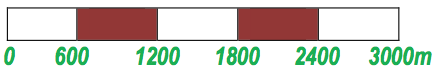
\includegraphics [width=3.4cm]{img-sol/t7-11}
 \end{enumerate}
\begin{enumerate}
\vspace{0.25cm}
\item[\fontfamily{phv}\selectfont\color{blue}\textbf{12. }] 
$6\times 40 = 240$ cm; $14\times 40= 560$ cm
\vspace{0.25cm}
\item[\fontfamily{phv}\selectfont\color{blue}\textbf{13. }] 
\begin {tabular}{|c|c|c|c|c|c|c|}\hline Magnitud A & 36 & 0,09 & 1,5& 12 & 0,125\tabularnewline \hline Magnitud B & 0,25 & 100 & 6 & 0,75 & 72\tabularnewline \hline \end {tabular}\par Raó $r'=36\cdot 0.25 = 9$ 
\vspace{0.25cm}
\item[\fontfamily{phv}\selectfont\color{blue}\textbf{14. }] 
$\frac {2,25\times 6}{1,5}=9$ panells de fusta
\vspace{0.25cm}
\item[\fontfamily{phv}\selectfont\color{blue}\textbf{15. }] 
$\frac {3\times 2 \times 6}{4 \times 5}=1,8$ hores. És a dir, tardarà 1 hora i 48 minuts.
\vspace{0.25cm}
\item[\fontfamily{phv}\selectfont\color{blue}\textbf{16. }] 
$\frac {900}{75}=12$ m.
\vspace{0.25cm}
\item[\fontfamily{phv}\selectfont\color{blue}\textbf{18. }] 
D-D $\frac {10}{5} \cdot \frac {2}{7} = \frac {8.45}{x}$ $\, \rightarrow \, x=14.79$ kg
\vspace{0.25cm}
\item[\fontfamily{phv}\selectfont\color{blue}\textbf{19. }] 
I-D $\frac {5}{2} \cdot \frac {1500}{5000} = \frac {6}{x}$ $\, \rightarrow \, x=0.8$ hores = 36 minuts
\vspace{0.25cm}
\item[\fontfamily{phv}\selectfont\color{blue}\textbf{20. }] 
I-D $\frac {8}{12} \cdot \frac {360}{620} = \frac {10}{x}$ $\, \rightarrow \, x=25.83$ dies
 \end{enumerate}
\vspace{0.3cm}

 \needspace{4\baselineskip} 

{\textbf{\em Pàgina 95}} \hrulefill
\begin{enumerate}
\vspace{0.25cm}
\item[\fontfamily{phv}\selectfont\color{blue}\textbf{22. }] 
I-I-D $\frac {24}{18} \cdot \frac {14}{6} \cdot \frac {300}{700}= \frac {6}{x}$ $\, \rightarrow \, x=4.5$ hores diàries
 \end{enumerate}
\begin{enumerate}
\vspace{0.25cm}
\item[\fontfamily{phv}\selectfont\color{blue}\textbf{23. }] 
D-I $\frac {34000}{35200} \cdot \frac {262}{284} = \frac {k}{x}$ $\, \rightarrow \, x=0.9551\, k$; si entenem $k=30$ dies $x=28.65$; si $k=31$ dies $x=29.6$; i si $k=365$ dies $x=348.61$ dies
\vspace{0.25cm}
\item[\fontfamily{phv}\selectfont\color{blue}\textbf{24. }] 
D-D $\frac {9}{15} \cdot \frac {10}{9} = \frac {2340}{x}$ $\, \rightarrow \, x=3510$ \euro {}/anuals
\vspace{0.25cm}
\item[\fontfamily{phv}\selectfont\color{blue}\textbf{25. }] 
I-D $\frac {8}{6} \cdot \frac {2}{3} = \frac {5}{x}$ $\, \rightarrow \, x=5.6$ dies
\vspace{0.25cm}
\item[\fontfamily{phv}\selectfont\color{blue}\textbf{26. }] 
D-D $\frac {4}{5} \cdot \frac {3}{2} = \frac {30000}{x}$ $\, \rightarrow \, x=25\,000$ còpies.
\vspace{0.25cm}
\item[\fontfamily{phv}\selectfont\color{blue}\textbf{27. }] 
Directa: $10 + 6+ 12+ 7 + 5=40$; $\frac {10}{40} 18000=4500$, $\frac {6}{40} 18000=2700$, $\frac {12}{40} 18000=5400$, $\frac {7}{40} 18000=3150$, $\frac {5}{40} 18000=2250$ \euro {}
\vspace{0.25cm}
\item[\fontfamily{phv}\selectfont\color{blue}\textbf{28. }] 
Directa: $12+15+18=45$. Rebran $\frac {12}{45}\,22200=5920$, $\frac {15}{45}\,22200=7400$, $\frac {18}{45}\,22200=8880$ \euro {}
\vspace{0.25cm}
\item[\fontfamily{phv}\selectfont\color{blue}\textbf{29. }] 
$32+24+14=70$; Rebran: $\frac {32}{70}\, 7350=3360$, $\frac {24}{70}\, 7350=2520$ i $\frac {14}{70}\, 7350=1470$ \euro {} 
 \end{enumerate}
\vspace{0.3cm}

 \needspace{4\baselineskip} 

{\textbf{\em Pàgina 96}} \hrulefill
\begin{enumerate}
\vspace{0.25cm}
\item[\fontfamily{phv}\selectfont\color{blue}\textbf{30. }] 
Inversa: $\frac {1}{12}+\frac {1}{15}+\frac {1}{18}=\frac {15}{180}+\frac {12}{180}+\frac {10}{180}=\frac {37}{180}$. Cadascun rebrà: $\frac {15}{37}\, 22200=9000$, $\frac {12}{37}\, 22200=7200$, $\frac {10}{37}\, 22200=6000$ \euro {}
 \end{enumerate}
\begin{enumerate}
\vspace{0.25cm}
\item[\fontfamily{phv}\selectfont\color{blue}\textbf{31. }] 
$\frac {20000}{105000} \,31500=6000$, $\frac {34000}{105000} \,31500=10200$, $\frac {51000}{105000} \,31500=15300$ \euro {}
\vspace{0.25cm}
\item[\fontfamily{phv}\selectfont\color{blue}\textbf{32. }] 
$\frac {3.5\cdot 4.8 + 5.2 \cdot 6}{3.5+5.2}=5.52$ \euro {} 
\vspace{0.25cm}
\item[\fontfamily{phv}\selectfont\color{blue}\textbf{33. }] 
$\frac {x\cdot 2.4 + 1.8 \cdot 4}{x+4}=2.13 \quad \rightarrow \quad x=\frac {1.32}{0.27}=4.89$ litres. 
\vspace{0.25cm}
\item[\fontfamily{phv}\selectfont\color{blue}\textbf{34. }] 
Inversa: $\frac {1}{6}+\frac {1}{5}+\frac {1}{2}+\frac {1}{1}=\frac {5}{30}+\frac {6}{30}+\frac {15}{30}+\frac {30}{30}=\frac {56}{30}$. Cadascú rebrà: $\frac {5}{56} \, 1400=125$, $\frac {6}{56} \, 1400=150$, $\frac {15}{56} \, 1400=375$, $\frac {30}{56} \, 1400=750$ punts
\vspace{0.25cm}


 \needspace{2\baselineskip} 

 \item[\fontfamily{phv}\selectfont\color{blue}\textbf{35}. ] 
 \begin{tasks}[column-sep=1em, item-indent=1.3333em](2)
	 \task* $\frac {3}{10}$; $\frac {3}{10}$
	 \task $\frac {4}{10}$
	 \task $134.4$; $134.4$
	 \task $179.2$ \euro {}
\end{tasks}
\vspace{0.25cm}
\item[\fontfamily{phv}\selectfont\color{blue}\textbf{36. }] 
$4\cdot 4.25+ 6\cdot 3.50 = 38$; $38\cdot 1.15=43.7$ \euro {}
 \end{enumerate}
\vspace{0.3cm}

 \needspace{4\baselineskip} 

{\textbf{\em Pàgina 97}} \hrulefill
\begin{enumerate}
\vspace{0.25cm}
\item[\fontfamily{phv}\selectfont\color{blue}\textbf{37. }] 
$1.04\cdot 250=260$ socis; $1.10\cdot 100 = 110$ \euro {} de quota anual; Ingressarà en total $260 \cdot 110 = 28600$ \euro {}
 \end{enumerate}
\begin{enumerate}
\vspace{0.25cm}
\item[\fontfamily{phv}\selectfont\color{blue}\textbf{38. }] 
$1.04 \cdot 0.40 \cdot 14= 5.82$ \euro {}
\vspace{0.25cm}


 \needspace{2\baselineskip} 

 \item[\fontfamily{phv}\selectfont\color{blue}\textbf{39}. ] 
 \begin{tasks}[column-sep=1em, item-indent=1.3333em](2)
	 \task* $0.75\cdot 8.60 + 0.650\cdot 5.80 = 10.22$ li ha costat; li tornaran $9.78$ \euro {}
	 \task* Tenia $0.2\,x = 10.22 \quad \rightarrow \quad x=51.10$ \euro {}
\end{tasks}
\vspace{0.25cm}


 \needspace{2\baselineskip} 

 \item[\fontfamily{phv}\selectfont\color{blue}\textbf{40}. ] 
 \begin{tasks}[column-sep=1em, item-indent=1.3333em](2)
	 \task* $0.78 \cdot 0.52 \cdot 148 = 60$ kg de sobrassada
	 \task* $0.021\cdot 60=1.26$ kg de sal; i $0.045\cdot 60=2.7$ kg de pebre vermell
\end{tasks}
\vspace{0.25cm}


 \needspace{2\baselineskip} 

 \item[\fontfamily{phv}\selectfont\color{blue}\textbf{41}. ] 
 \begin{tasks}[column-sep=1em, item-indent=1.3333em](2)
	 \task* $0.4\cdot 30 + 0.25\cdot 28 + 0.75 \cdot 32 = 43$ alumnes participen a la coral
	 \task* El total d'alumnes és $30+28+32=90$; $\frac {43}{90}\cdot 100=47.78$ \% del total
\end{tasks}
\vspace{0.25cm}


 \needspace{2\baselineskip} 

 \item[\fontfamily{phv}\selectfont\color{blue}\textbf{42}. ] 
 \begin{tasks}[column-sep=1em, item-indent=1.3333em](2)
	 \task* $100-78-21-0.04=0.96$ \% de gasos nobles
	 \task* $\frac {0.96}{100}\,500 \cdot 15 \cdot 60 = 4320$ ml/hora = 4.32 l/hora
\end{tasks}
\vspace{0.25cm}


 \needspace{2\baselineskip} 

 \item[\fontfamily{phv}\selectfont\color{blue}\textbf{43}. ] 
 \begin{tasks}[column-sep=1em, item-indent=1.3333em](2)
	 \task* $0.8\cdot 1.16\cdot 500=464$ \euro {}
	 \task* $\frac {0.75\cdot 464}{12}=29$ \euro {}/mensuals
\end{tasks}
 \end{enumerate}
\vspace{0.3cm}

 \needspace{4\baselineskip} 

{\textbf{\em Pàgina 98}} \hrulefill
\begin{enumerate}
\vspace{0.25cm}
\item[\fontfamily{phv}\selectfont\color{blue}\textbf{44. }] 
$\frac {105000\cdot 4.8 \cdot 750}{36000}=10500$ \euro {}
 \end{enumerate}
\begin{enumerate}
\vspace{0.25cm}
\item[\fontfamily{phv}\selectfont\color{blue}\textbf{45. }] 
$39500 \left (1+\frac {5}{100}\right )^{12} = 70936.32$ \euro {}
\vspace{0.25cm}
\item[\fontfamily{phv}\selectfont\color{blue}\textbf{46. }] 
$\frac {C \cdot 1.8 \cdot 6}{100}=777.6$; $C=7200$ \euro {}
\vspace{0.25cm}
\item[\fontfamily{phv}\selectfont\color{blue}\textbf{47. }] 
\begin {tabular}{|c|c|c|c|c|c|} \hline \textbf {l.} & 6,25 & 5 & 0,75 & 1,4 &\tabularnewline \hline \textbf {\euro {}} & 18,75 & 15 & 2,25 &4,2 & 4,5\tabularnewline \hline \end {tabular}\par $k=\frac {0.75}{2.25}=\frac {1}{3}$ 
\vspace{0.25cm}
\item[\fontfamily{phv}\selectfont\color{blue}\textbf{48. }] 
136.8 \euro {}
\vspace{0.25cm}
\item[\fontfamily{phv}\selectfont\color{blue}\textbf{49. }] 
Suposant 4 setmanes per mes: $82\cdot 8 =656$ \euro {}. Suposant 9 setmanes en total, $82\cdot 9 =738$ \euro {}. Més precís (per dies): $\frac {82\cdot 61}{7}=714.57$ \euro {} 
\vspace{0.25cm}
\item[\fontfamily{phv}\selectfont\color{blue}\textbf{50. }] 
50 cadires
\vspace{0.25cm}
\item[\fontfamily{phv}\selectfont\color{blue}\textbf{51. }] 
9,3 = 10 viatges
\vspace{0.25cm}
\item[\fontfamily{phv}\selectfont\color{blue}\textbf{52. }] 
84 kg
\vspace{0.25cm}
\item[\fontfamily{phv}\selectfont\color{blue}\textbf{53. }] 
\begin {tabular}{|c|c|c|c|c|c|} \toprule \textbf {A} & 12,6 & 16,2 & 0,18 & 4,14 & 4,86\tabularnewline \midrule \textbf {B} & 7 & 9 & 0,1 & 2,3 & 2,7\tabularnewline \bottomrule \end {tabular}
\vspace{0.25cm}
\item[\fontfamily{phv}\selectfont\color{blue}\textbf{54. }] 
293,12 \euro {}
\vspace{0.25cm}
\item[\fontfamily{phv}\selectfont\color{blue}\textbf{55. }] 
1702,40 \euro {}
\vspace{0.25cm}
\item[\fontfamily{phv}\selectfont\color{blue}\textbf{56. }] 
30 \%
\vspace{0.25cm}
\item[\fontfamily{phv}\selectfont\color{blue}\textbf{57. }] 
620 \euro {}
 \end{enumerate}
\vspace{0.3cm}

 \needspace{4\baselineskip} 

{\textbf{\em Pàgina 99}} \hrulefill
\begin{enumerate}
\vspace{0.25cm}
\item[\fontfamily{phv}\selectfont\color{blue}\textbf{58. }] 
S'han estalviat 420 \euro {}; El percentatge és 12 \%
 \end{enumerate}
\begin{enumerate}
\vspace{0.25cm}
\item[\fontfamily{phv}\selectfont\color{blue}\textbf{59. }] 
El preu sense IVA és 750 \euro {}
\vspace{0.25cm}
\item[\fontfamily{phv}\selectfont\color{blue}\textbf{60. }] 
24 \%
\vspace{0.25cm}
\item[\fontfamily{phv}\selectfont\color{blue}\textbf{61. }] 
1 : 3400000
\vspace{0.25cm}
\item[\fontfamily{phv}\selectfont\color{blue}\textbf{62. }] 
6 km llarg i 1.25 km d'ample; 1:250000; 1.5 cm
\vspace{0.25cm}
\item[\fontfamily{phv}\selectfont\color{blue}\textbf{63. }] 
\begin {tabular}{|c|c|c|c|c|c|} \hline \textbf { A} & 4 & 7,5 & 500 & 3,6 & 9\tabularnewline \hline \textbf { B} & 22.5 & 12 & 0,18 & 25& 10\tabularnewline \hline \end {tabular}\par $k'=7.5\times 12 = 90$
\vspace{0.25cm}
\item[\fontfamily{phv}\selectfont\color{blue}\textbf{64. }] 
Espai recorregut 420 km. Velocitat 105 km/h
\vspace{0.25cm}
\item[\fontfamily{phv}\selectfont\color{blue}\textbf{65. }] 
12 setmanes; 8 setmanes; 12 setmanes
\vspace{0.25cm}
\item[\fontfamily{phv}\selectfont\color{blue}\textbf{66. }] 
42 kg en total; Número de paquets 21.
\vspace{0.25cm}
\item[\fontfamily{phv}\selectfont\color{blue}\textbf{67. }] 
16 operaris
\vspace{0.25cm}
\item[\fontfamily{phv}\selectfont\color{blue}\textbf{68. }] 
12 dies
\vspace{0.25cm}
\item[\fontfamily{phv}\selectfont\color{blue}\textbf{69. }] 
7 dies
\vspace{0.25cm}
\item[\fontfamily{phv}\selectfont\color{blue}\textbf{70. }] 
84000 \euro {}; 54600 \euro {}; 29400 \euro {}
\vspace{0.25cm}
\item[\fontfamily{phv}\selectfont\color{blue}\textbf{71. }] 
1320 \euro {}; 960 \euro {}; 840 \euro {}
\vspace{0.25cm}
\item[\fontfamily{phv}\selectfont\color{blue}\textbf{72. }] 
Suposant un repartiment proporcional de 177.5 \euro {}, cadascú ha de pagar: 15.21 \euro {}; 25.36 \euro {}; 35.5 \euro {}; 40.57 \euro {}; 60.86 \euro {}.
\vspace{0.25cm}
\item[\fontfamily{phv}\selectfont\color{blue}\textbf{73. }] 
9791666,7 \euro {}; 5875000 \euro {}; 7833333.3 \euro {}
\vspace{0.25cm}
\item[\fontfamily{phv}\selectfont\color{blue}\textbf{74. }] 
Preu per kg: 13.2 \euro {}; preu del paquet 3.3 \euro {}
\vspace{0.25cm}
\item[\fontfamily{phv}\selectfont\color{blue}\textbf{75. }] 
Preu per litre de mescla: 1.79 \euro {}; Preu per botella: 2.69 \euro {}; Amb l'augment 3.75 \euro {}.
 \end{enumerate}
\vspace{0.3cm}

 \needspace{4\baselineskip} 

{\textbf{\em Pàgina 100}} \hrulefill
\begin{enumerate}
\vspace{0.25cm}
\item[\fontfamily{phv}\selectfont\color{blue}\textbf{76. }] 
4628,57 \euro {}
 \end{enumerate}
\begin{enumerate}
\vspace{0.25cm}
\item[\fontfamily{phv}\selectfont\color{blue}\textbf{77. }] 
28956 \euro {}
\vspace{0.25cm}
\item[\fontfamily{phv}\selectfont\color{blue}\textbf{78. }] 
16 mesos
\vspace{0.25cm}
 \item[$\bullet$ ] {\fontfamily{phv}\selectfont\color{blue}\textbf{Autoavaluació:}. }

\vspace{0.25cm}
\item[\fontfamily{phv}\selectfont\color{blue}\textbf{1. }]  \scalebox{0.6}{\simbolclau } 
160; 0.3; 90; 2000
\vspace{0.25cm}
\item[\fontfamily{phv}\selectfont\color{blue}\textbf{2. }]  \scalebox{0.6}{\simbolclau } 
1687.5 \euro {}
\vspace{0.25cm}
\item[\fontfamily{phv}\selectfont\color{blue}\textbf{3. }]  \scalebox{0.6}{\simbolclau } 
12.5 \%
\vspace{0.25cm}
\item[\fontfamily{phv}\selectfont\color{blue}\textbf{4. }]  \scalebox{0.6}{\simbolclau } 
480 botelles
\vspace{0.25cm}
\item[\fontfamily{phv}\selectfont\color{blue}\textbf{5. }]  \scalebox{0.6}{\simbolclau } 
16 t i 12.8 t
\vspace{0.25cm}
\item[\fontfamily{phv}\selectfont\color{blue}\textbf{6. }]  \scalebox{0.6}{\simbolclau } 
1:30\,000
\vspace{0.25cm}
\item[\fontfamily{phv}\selectfont\color{blue}\textbf{7. }]  \scalebox{0.6}{\simbolclau } 
5 rotllos
\vspace{0.25cm}
\item[\fontfamily{phv}\selectfont\color{blue}\textbf{8. }]  \scalebox{0.6}{\simbolclau } 
1,05\euro {}
\vspace{0.25cm}
\item[\fontfamily{phv}\selectfont\color{blue}\textbf{9. }]  \scalebox{0.6}{\simbolclau } 
64 camions
\vspace{0.25cm}
\item[\fontfamily{phv}\selectfont\color{blue}\textbf{10. }]  \scalebox{0.6}{\simbolclau } 
16329,35 \euro {}
 \end{enumerate}
\vfill\null
\columnbreak
\def\currentname{Solucions del Tema 8}
\vspace*{0.75cm}

 
 \needspace{5\baselineskip} 
 \scalebox{1.25}{\heading{Solucions del Tema 8}}

\vspace*{0.4cm}
\phantomsection \addcontentsline{toc}{section}{Solucions del Tema 8}
\vspace{0.3cm}

 \needspace{4\baselineskip} 

{\textbf{\em Pàgina 102}} \hrulefill
\begin{enumerate}
\vspace{0.25cm}
\item[\fontfamily{phv}\selectfont\color{blue}\textbf{1. }] 
a) A(--4,2); B(--2,0); C(--3,--2); D(--1, 3); E(1,2); F(1,--1); G(3,0); H(3,4); I(4,--2); J(5,--3)
 \end{enumerate}
\vspace{0.3cm}

 \needspace{4\baselineskip} 

{\textbf{\em Pàgina 103}} \hrulefill
\begin{enumerate}
\vspace{0.25cm}
\item[\fontfamily{phv}\selectfont\color{blue}\textbf{3. }] 
Tots ells es troben sobre l'eix de les ordenades.
 \end{enumerate}
\begin{enumerate}
\vspace{0.25cm}
\item[\fontfamily{phv}\selectfont\color{blue}\textbf{4. }] 
Per exemple (--3, --2); (--1, --5); (--2;--2). Les dues coordenades són negatives.
\vspace{0.25cm}
\item[\fontfamily{phv}\selectfont\color{blue}\textbf{5. }] 
Per exemple (0,3); (0,--5); (0,1). Tots tenen la primera coordenada igual a zero.
\vspace{0.25cm}


 \needspace{2\baselineskip} 

 \item[\fontfamily{phv}\selectfont\color{blue}\textbf{6}. ] 
 \begin{tasks}[column-sep=1em, item-indent=1.3333em](2)
	 \task Sí
	 \task No
	 \task No
	 \task Sí
	 \task Sí
	 \task Sí
	 \task No
\end{tasks}
\vspace{0.25cm}


 \needspace{2\baselineskip} 

 \item[\fontfamily{phv}\selectfont\color{blue}\textbf{8}. ] 
 \begin{tasks}[column-sep=1em, item-indent=1.3333em](1)
	 \task*  No (pot tenir més d'un divisor)
	 \task* Sí (cada circumferència només té 1 centre)
\end{tasks}
\vspace{0.25cm}
\item[\fontfamily{phv}\selectfont\color{blue}\textbf{9. }] 
No és funció. Per una $x=-13$, trobam dos valors de $y=-15$ i $3$
 \end{enumerate}
\vspace{0.3cm}

 \needspace{4\baselineskip} 

{\textbf{\em Pàgina 104}} \hrulefill
\begin{enumerate}
\vspace{0.25cm}


 \needspace{2\baselineskip} 

 \item[\fontfamily{phv}\selectfont\color{blue}\textbf{10}. ] 
 \begin{tasks}[column-sep=1em, item-indent=1.3333em](1)
	 \task 125 o 160 cm
	 \task 13 anys
	 \task* No és una relació funcional perquè per una edat trobam diverses altures
	 \task* Tampoc és funcional perquè una una altura trobam diferents edats.
\end{tasks}
 \end{enumerate}
\begin{enumerate}
\vspace{0.25cm}


 \needspace{2\baselineskip} 

 \item[\fontfamily{phv}\selectfont\color{blue}\textbf{11}. ] 
 \begin{tasks}[column-sep=1em, item-indent=1.3333em](2)
	 \task $m=2$
	 \task $m=\frac {3}{2}$
	 \task $m=-3$
	 \task $m=\frac {-4}{5}$
\end{tasks}
\vspace{0.25cm}
\item[\fontfamily{phv}\selectfont\color{blue}\textbf{12. }] 
$y=3x$; $y=-2x$; $y=\frac {1}{2}x$ 
\vspace{0.25cm}


 \needspace{2\baselineskip} 

 \item[\fontfamily{phv}\selectfont\color{blue}\textbf{13}. ] 
 \begin{tasks}[column-sep=1em, item-indent=1.3333em](1)
	 \task $m=\frac {1}{3}$; $y=\frac {1}{3}x$
	 \task $m=2$; $y=2x$
	 \task $m=-5/2$; $y=-\frac {5}{2}x$
	 \task $m=-4/3$; $y=-\frac {4}{3}x$
\end{tasks}
\vspace{0.25cm}
\item[\fontfamily{phv}\selectfont\color{blue}\textbf{14. }] 
6.75 \euro {}, 13.5 \euro {}, 16.88 \euro {}. En general $y=1.35 x$
 \end{enumerate}
\vspace{0.3cm}

 \needspace{4\baselineskip} 

{\textbf{\em Pàgina 105}} \hrulefill
\begin{enumerate}
\vspace{0.25cm}
\item[\fontfamily{phv}\selectfont\color{blue}\textbf{15. }] 
 \begin {tabular}{|c|c|c|c|c|c|} \hline \cellcolor {lightgray}\textbf {\euro {}} & 2 & 5 & 10 & 27 & 60 \\ [0.3cm] \hline \cellcolor {lightgray}\textbf {\$} &2.74 & 6.85 & 13.70 & 36.99 & 82.20 \\ [0.3cm] \hline \end {tabular}\par En general: $y=1.37 x$. És una funció.\par Si aplicam comissió: $y=1.37 (x - 1.5)=1.37 x -2.06$; igual que abans però et lleven \$ 2.06 
 \end{enumerate}
\begin{enumerate}
\vspace{0.25cm}
\item[\fontfamily{phv}\selectfont\color{blue}\textbf{16. }] 
\begin {tabular}{|c|c|c|c|c|c|} \hline \cellcolor {lightgray}\textbf {h} & 0 & 3 & 6 & 9 & 12 \\ [0.3cm] \hline \cellcolor {lightgray}\textbf {V} & 0 & 151 & 301.4 & 452 & 603 \\ [0.3cm] \hline \end {tabular}\par $V=\pi r^2 h = 50.24 h$. $h=\frac {V}{50.24}$. 1 dl = 100 cm$^3$, aleshores aproximadament s'ha de col·locar la marca a 2 cm d'altura. 
\vspace{0.25cm}


 \needspace{2\baselineskip} 

 \item[\fontfamily{phv}\selectfont\color{blue}\textbf{17}. ] 
 \begin{tasks}[column-sep=1em, item-indent=1.3333em](1)
	 \task $d=78\pi n$
	 \task* Solució gràfica: una recta que passa per l'origen i té pendent $78\pi =245.04$
	 \task* $d=78\pi \,1000=245\,044$ cm =2.45 km
	 \task 2856.6 voltes
\end{tasks}
\vspace{0.25cm}


 \needspace{2\baselineskip} 

 \item[\fontfamily{phv}\selectfont\color{blue}\textbf{18}. ] 
 \begin{tasks}[column-sep=1em, item-indent=1.3333em](1)
	 \task Pendent 3; ordenada 2
	 \task Pendent 1; ordenada --3
	 \task Pendent --2; ordenada --1
	 \task* Pendent $-\frac {1}{2}$; ordenada 4
\end{tasks}
\vspace{0.25cm}
\item[\fontfamily{phv}\selectfont\color{blue}\textbf{19. }] 
Són rectes paral·leles.
 \end{enumerate}
\vspace{0.3cm}

 \needspace{4\baselineskip} 

{\textbf{\em Pàgina 106}} \hrulefill
\begin{enumerate}
\vspace{0.25cm}


 \needspace{2\baselineskip} 

 \item[\fontfamily{phv}\selectfont\color{blue}\textbf{20}. ] 
 \begin{tasks}[column-sep=1em, item-indent=1.3333em](1)
	 \task* Totes les rectes són paral·leles (i decreixents)
	 \task* $y=-2x$; $y=-2x+3$; $y=-2x-4$. Totes elles comparteixen el mateix pendent ($m=-2$) 
\end{tasks}
 \end{enumerate}
\begin{enumerate}
\vspace{0.25cm}


 \needspace{2\baselineskip} 

 \item[\fontfamily{phv}\selectfont\color{blue}\textbf{21}. ] 
 \begin{tasks}[column-sep=1em, item-indent=1.3333em](2)
	 \task $y=2x+3$
	 \task $y=-x+4$
	 \task $y=0$
	 \task $y=-2x+1$
\end{tasks}
\vspace{0.25cm}


 \needspace{2\baselineskip} 

 \item[\fontfamily{phv}\selectfont\color{blue}\textbf{22}. ] 
 \begin{tasks}[column-sep=1em, item-indent=1.3333em](2)
	 \task $y=3x$
	 \task $y=-x+5$
	 \task $y=2x-3$
\end{tasks}
\vspace{0.25cm}
\item[\fontfamily{phv}\selectfont\color{blue}\textbf{23. }] 
\begin {tabular}[]{|c|c|c|c|c|c|c|}\hline $t$ & 0 & 1 & 2 & 3 & 4 & 5 \\ \hline $e$ & 20 & 25 & 30 & 35 & 40 & 45 \\ \hline \end {tabular} \par És una recta que passa per (0,20) i té pendent 5. No té sentit per temps negatius. 
\vspace{0.25cm}


 \needspace{2\baselineskip} 

 \item[\fontfamily{phv}\selectfont\color{blue}\textbf{24}. ] 
 \begin{tasks}[column-sep=1em, item-indent=1.3333em](1)
	 \task --7.6 $^\circ $C
	 \task 7020 m
	 \task $t=9-\frac {a}{180}$
	 \task* $t=12-\frac {a}{180}$. Les dues funcions afins representen rectes paral·les.
\end{tasks}
 \end{enumerate}
\vspace{0.3cm}

 \needspace{4\baselineskip} 

{\textbf{\em Pàgina 107}} \hrulefill
\begin{enumerate}
\vspace{0.25cm}
\item[\fontfamily{phv}\selectfont\color{blue}\textbf{25. }] 
Fórmula 1: $y=3000d$. Fórmula 2: $y=200d + 7x$. El cost de la fórmula 1: 3000 \euro {}. El cost de la fórmula 2: 2000+7000=9000 \euro {}. En general és més econòmica l'opció 1; però si hem de fer menys de 14 km diaris surt més econòmica la fórmula 2.
 \end{enumerate}
\begin{enumerate}
\vspace{0.25cm}
\item[\fontfamily{phv}\selectfont\color{blue}\textbf{26. }] 
Les parelles de rectes són perpendiculars. La condició que han de complir és $m \cdot m' = -1$
\vspace{0.25cm}
\item[\fontfamily{phv}\selectfont\color{blue}\textbf{27. }] 
$y=4x+6$
\vspace{0.25cm}
\item[\fontfamily{phv}\selectfont\color{blue}\textbf{28. }] 
No estan alineats. Els punts A,B estan sobre una recta de pendent 5/4, mentre que els punts B,C estan sobre una recta de 1.
\vspace{0.25cm}
\item[\fontfamily{phv}\selectfont\color{blue}\textbf{29. }] 
a), b) còncaves. c), d) convexes.\par 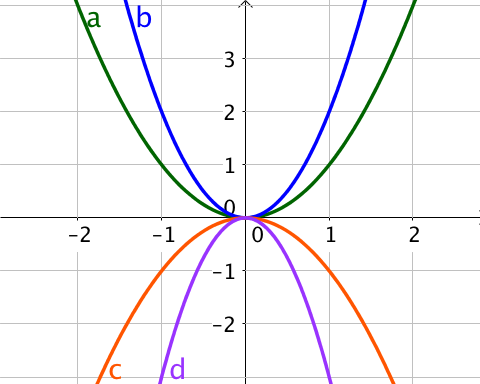
\includegraphics [width=0.45\textwidth ]{img-sol/t8-29}
\vspace{0.25cm}
\item[\fontfamily{phv}\selectfont\color{blue}\textbf{30. }] 
Gràfics:\par 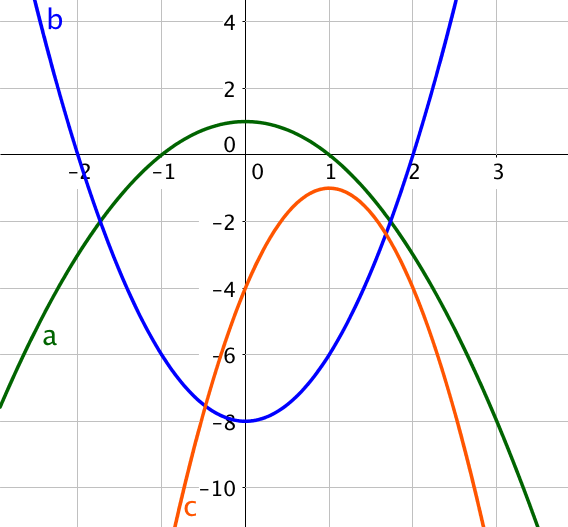
\includegraphics [width=0.38\textwidth ]{img-sol/t8-30}
 \end{enumerate}
\vspace{0.3cm}

 \needspace{4\baselineskip} 

{\textbf{\em Pàgina 108}} \hrulefill
\begin{enumerate}
\vspace{0.25cm}


 \needspace{2\baselineskip} 

 \item[\fontfamily{phv}\selectfont\color{blue}\textbf{31}. ] 
 \begin{tasks}[column-sep=1em, item-indent=1.3333em](2)
	 \task $V(-2,4)$
	 \task $V(2,-2)$
	 \task $V(1,0)$
	 \task* $V(-\frac {3}{2},-\frac {9}{2})$
\end{tasks}
 \end{enumerate}
\begin{enumerate}
\vspace{0.25cm}


 \needspace{2\baselineskip} 

 \item[\fontfamily{phv}\selectfont\color{blue}\textbf{32}. ] 
 \begin{tasks}[column-sep=1em, item-indent=1.3333em](1)
	 \task* $V(-4,-29)$; talls $(-9.39,0)$ $(1.39,0)$ $(0,-13)$
	 \task* $V(4,3)$; talls $(2.27,0)$ $(5.73,0)$ $(0,-13)$
	 \task* $V(2,-2)$; talls $(0.59,0)$ $(3.41,0)$ $(0,2)$
	 \task* $V(-3,-9)$; talls $(-6,0)$ $(0,0)$ 
\end{tasks}
\vspace{0.25cm}


 \needspace{2\baselineskip} 

 \item[\fontfamily{phv}\selectfont\color{blue}\textbf{33}. ] 
 \begin{tasks}[column-sep=1em, item-indent=1.3333em](2)
	 \task còncava
	 \task menor
	 \task convexa
	 \task major
\end{tasks}
\vspace{0.25cm}


 \needspace{2\baselineskip} 

 \item[\fontfamily{phv}\selectfont\color{blue}\textbf{34}. ] 
 \begin{tasks}[column-sep=1em, item-indent=1.3333em](2)
	 \task* Respecte el centre el pont $y=0.0001193 x^2$
	 \task 119.27 peus d'altura
\end{tasks}
\vspace{0.25cm}
\item[\fontfamily{phv}\selectfont\color{blue}\textbf{35. }] 
$y=(x-5)^2+3 = x^2-10x+28$. El nou vèrtex és $V(5,3)$.
 \end{enumerate}
\vspace{0.3cm}

 \needspace{4\baselineskip} 

{\textbf{\em Pàgina 109}} \hrulefill
\begin{enumerate}
\vspace{0.25cm}
\item[\fontfamily{phv}\selectfont\color{blue}\textbf{36. }] 
$A=-x^2+50x$. És una funció quadràtica que talla a l'eix de les abscisses a $x=0$ i $x=50$ i vèrtex $V(25, 625)$ 
 \end{enumerate}
\begin{enumerate}
\vspace{0.25cm}
\item[\fontfamily{phv}\selectfont\color{blue}\textbf{37. }] 
$V=20x^2$
\vspace{0.25cm}
\item[\fontfamily{phv}\selectfont\color{blue}\textbf{38. }] 
$V = (32 – 2x) \cdot (22 – 2x)\cdot x$; $V(3) = 1248$ cm$^3$; $V(2) = 1 008$ cm$^3$
\vspace{0.25cm}


 \needspace{2\baselineskip} 

 \item[\fontfamily{phv}\selectfont\color{blue}\textbf{39}. ] 
 \begin{tasks}[column-sep=1em, item-indent=1.3333em](1)
	 \task* Gràfica 1: Dom $f=\Re $; Rec $f=[1,+\infty ]$; Simetria parell; Talla eix OY a (0,1); És contínua; És decreixent $(-\infty ,0)$ i creixent de $(0,+\infty )$; Té un mínim a (0,1)
	 \task* Gràfica 2: Dom $f=\Re $; Rec $f=\Re $; Simetria senar; Talla eix OX (--2,0) (0,0) (2,0) i l'eix OY a (0,0); És contínua; És decreixent $(-1,1)$ i creixent de $(-\infty ,-1)\cup (1,+\infty )$; Té un màxim a (-1,3) i un mínim a (1,-3)
	 \task* Gràfica 3: Dom $f=\Re $-{0}; Rec $f=\Re -{0}$; Simetria senar; No hi ha talls amb eixos; No és contínua a x=0; Sempre decreixent; No té extrems
	 \task* Gràfica 4: Dom $f=\Re $; Rec $f=[-1,1]$; Simetria senar; Talla l'eix OX a cada nombre enter; És contínua; És periòdica amb període 2. Presenta màxims a $0.5+2n$ i mínims $1.5+2n$ 
\end{tasks}
\vspace{0.25cm}
\item[\fontfamily{phv}\selectfont\color{blue}\textbf{40. }] 
 D'aquí a 7 anys cobrarà 50 euros. És una funció esglaonada, ja que cobra el mateix durant tot un any, i després augmenta 5 euros:\par $P =\left \{ \begin {array}{cl} 20 & \text {1r any} \\ 25 & \text {2n any} \\ 30 & \text {3r any} \\ \cdots & \\ 20 + 5(n-1) & \text {any }n \end {array} \right .$
\vspace{0.25cm}


 \needspace{2\baselineskip} 

 \item[\fontfamily{phv}\selectfont\color{blue}\textbf{41}. ] 
 \begin{tasks}[column-sep=1em, item-indent=1.3333em](1)
	 \task El consum en litres/100 km
	 \task La velocitat en km/h
	 \task* Gasoil: 9.50 l/100 km; Benzina: 13 l/100 km
	 \task* Gasoil: 135 km/h; Benzina: 105 km/h
	 \task* El consum en general augment amb la velocitat i sempre és major el consum de benzina que no pas el de Gasoil.
\end{tasks}
 \end{enumerate}
\vspace{0.3cm}

 \needspace{4\baselineskip} 

{\textbf{\em Pàgina 110}} \hrulefill
\begin{enumerate}
\vspace{0.25cm}


 \needspace{2\baselineskip} 

 \item[\fontfamily{phv}\selectfont\color{blue}\textbf{42}. ] 
 \begin{tasks}[column-sep=1em, item-indent=1.3333em](1)
	 \task 12 hores
	 \task* 3 hores de descans: entre les 14 i les 15 i entre les 18 i les 19 hores
	 \task Es van recórrer 80 km
	 \task* En tots els altres excepte quan descansaven
	 \task lliure
\end{tasks}
 \end{enumerate}
\begin{enumerate}
\vspace{0.25cm}


 \needspace{2\baselineskip} 

 \item[\fontfamily{phv}\selectfont\color{blue}\textbf{43}. ] 
 \begin{tasks}[column-sep=1em, item-indent=1.3333em](1)
	 \task Sí. Es funcional
	 \task* Independent: temps; Dependent: Velocitat
	 \task* Anava a 90 km/h; Anava a 40 km/h als 20 i 110 minuts
	 \task* Creixent $(0,40)\cup (50,70)$; Decreixent $(40,50)\cup (70,80)\cup (100,120)$; Constant: $(80,100)$ durant 20 minuts
	 \task* Els màxims relatius són (40,80) i (70,120); El mínim relatiu és (50,60). 
\end{tasks}
 \end{enumerate}
\vspace{0.3cm}

 \needspace{4\baselineskip} 

{\textbf{\em Pàgina 111}} \hrulefill
\begin{enumerate}
\vspace{0.25cm}


 \needspace{2\baselineskip} 

 \item[\fontfamily{phv}\selectfont\color{blue}\textbf{44}. ] 
 \begin{tasks}[column-sep=1em, item-indent=1.3333em](1)
	 \task $y=0.03 x$
	 \task $1.65$ \euro {}
	 \task 80 minuts
\end{tasks}
 \end{enumerate}
\begin{enumerate}
\vspace{0.25cm}
\item[\fontfamily{phv}\selectfont\color{blue}\textbf{45. }] 
Gràfica: \par 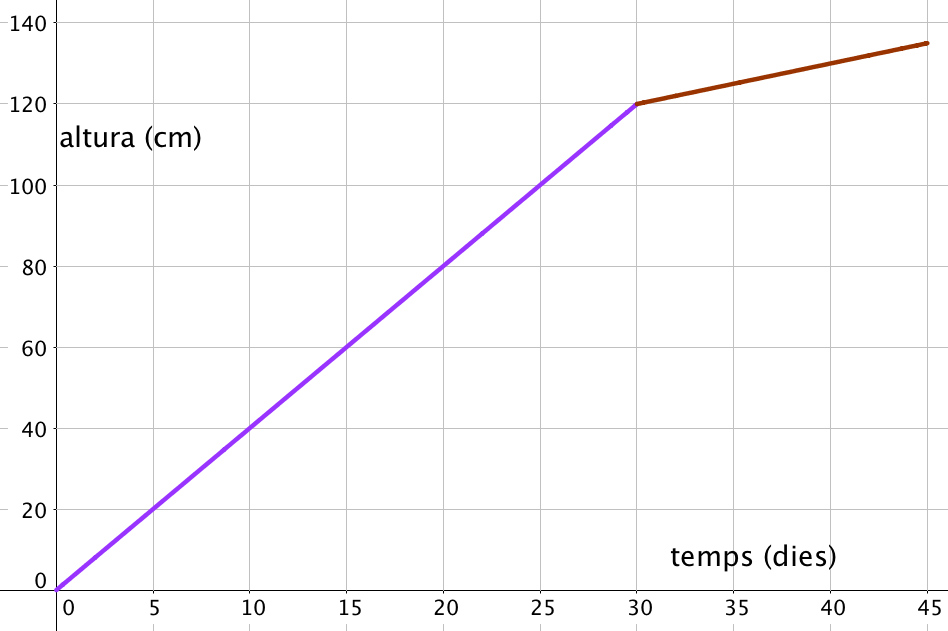
\includegraphics [width=0.45\textwidth ]{img-sol/t8-45}
\vspace{0.25cm}
 \item[$\bullet$ ] {\fontfamily{phv}\selectfont\color{blue}\textbf{Autoavaluació:}. }

\vspace{0.25cm}
\item[\fontfamily{phv}\selectfont\color{blue}\textbf{1. }]  \scalebox{0.6}{\simbolclau } 
\textbf {--6.} Autoavaluació: 1b; 2d; 3a; 4c; 5b; 6b
 \end{enumerate}
\vfill\null
\columnbreak
\def\currentname{Solucions del Tema 9}
\vspace*{0.75cm}

 
 \needspace{5\baselineskip} 
 \scalebox{1.25}{\heading{Solucions del Tema 9}}

\vspace*{0.4cm}
\phantomsection \addcontentsline{toc}{section}{Solucions del Tema 9}
\vspace{0.3cm}

 \needspace{4\baselineskip} 

{\textbf{\em Pàgina 114}} \hrulefill
\begin{enumerate}
\vspace{0.25cm}


 \needspace{2\baselineskip} 

 \item[$\bullet$ ] {\fontfamily{phv}\selectfont\color{blue}\textbf{Avaluació inicial}. } 
 \begin{tasks}[column-sep=1em, item-indent=1.3333em](1)
	 \task* La raó és $r=\dfrac {3}{2}=1.5$. Han ampliat un 150 \%
	 \task Les mesures són 1.5 cm i 6 cm
	 \task* L'àrea del cercle ampliat és 7.1 cm$^2$
	 \task $A=1079$ cm$^2$.
\end{tasks}
 \end{enumerate}
\vspace{0.3cm}

 \needspace{4\baselineskip} 

{\textbf{\em Pàgina 115}} \hrulefill
\begin{enumerate}
\vspace{0.25cm}


 \needspace{2\baselineskip} 

 \item[\fontfamily{phv}\selectfont\color{blue}\textbf{1}. ] 
 \begin{tasks}[column-sep=1em, item-indent=1.3333em](1)
	 \task* Sí perquè tenen tots els angles iguals
	 \task* No perquè els seus angles respectius són 70; 55; 55 i 80; 50; 50
	 \task* Si perquè tenen un angle igual i els costats que els formen són proporcionals (la meitat). No perquè $\dfrac {a'}{a} = \dfrac {b'}{b} = 2.5$ però $\dfrac {c'}{c} = 3.5$
\end{tasks}
 \end{enumerate}
\begin{enumerate}
\vspace{0.25cm}


 \needspace{2\baselineskip} 

 \item[\fontfamily{phv}\selectfont\color{blue}\textbf{2}. ] 
 \begin{tasks}[column-sep=1em, item-indent=1.3333em](2)
	 \task $c'=8$ cm
	 \task $c'=8$ cm
\end{tasks}
\vspace{0.25cm}
\item[\fontfamily{phv}\selectfont\color{blue}\textbf{3. }] 
L'edifici mesura 12.8 m.
\vspace{0.25cm}
\item[\fontfamily{phv}\selectfont\color{blue}\textbf{4. }] 
Primer trobam la raó de semblança $\dfrac {60}{(6+7+7)}=3$. Els nous costats s'obtenen de multiplicar per 3 els originals: 18 cm, 21 cm i 21 cm
 \end{enumerate}
\vspace{0.3cm}

 \needspace{4\baselineskip} 

{\textbf{\em Pàgina 116}} \hrulefill
\begin{enumerate}
\vspace{0.25cm}


 \needspace{2\baselineskip} 

 \item[\fontfamily{phv}\selectfont\color{blue}\textbf{5}. ]  \scalebox{0.6}{\simbolclau } 
 \begin{tasks}[column-sep=1em, item-indent=1.3333em](1)
	 \task $x=4$ i $y=3$ cm
	 \task $x=6$ i $y=18$ cm
\end{tasks}
 \end{enumerate}
\begin{enumerate}
\vspace{0.25cm}
\item[\fontfamily{phv}\selectfont\color{blue}\textbf{6. }] 
Esquema:\par 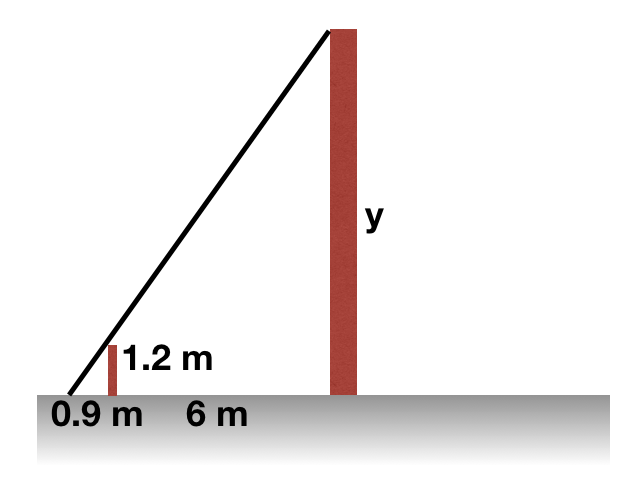
\includegraphics [width=0.3\textwidth ]{img-sol/t9-5}\par El pal mesura 8 m i el cable 10 m.
\vspace{0.25cm}


 \needspace{2\baselineskip} 

 \item[\fontfamily{phv}\selectfont\color{blue}\textbf{7}. ] 
 \begin{tasks}[column-sep=1em, item-indent=1.3333em](1)
	 \task $x=2$; $y=1.375$ cm
	 \task $x=9$; $y=3$; $z=4.5$ cm
\end{tasks}
\vspace{0.25cm}
\item[\fontfamily{phv}\selectfont\color{blue}\textbf{8. }] 
Sí. La hipotenusa ha de mesurar 13 cm
 \end{enumerate}
\vspace{0.3cm}

 \needspace{4\baselineskip} 

{\textbf{\em Pàgina 117}} \hrulefill
\begin{enumerate}
\vspace{0.25cm}


 \needspace{2\baselineskip} 

 \item[\fontfamily{phv}\selectfont\color{blue}\textbf{9}. ] 
 \begin{tasks}[column-sep=1em, item-indent=1.3333em](2)
	 \task 10 cm
	 \task 5 m
	 \task 17 dm
	 \task 25.4 km
\end{tasks}
 \end{enumerate}
\begin{enumerate}
\vspace{0.25cm}


 \needspace{2\baselineskip} 

 \item[\fontfamily{phv}\selectfont\color{blue}\textbf{10}. ] 
 \begin{tasks}[column-sep=1em, item-indent=1.3333em](2)
	 \task 24 cm
	 \task 15 m
	 \task 12 dm
	 \task 13.5 km
\end{tasks}
\vspace{0.25cm}
\item[\fontfamily{phv}\selectfont\color{blue}\textbf{11. }]  \scalebox{0.6}{\simbolclau } 
$x=8$ cm
\vspace{0.25cm}
\item[\fontfamily{phv}\selectfont\color{blue}\textbf{12. }] 
$A=\frac {81}{4}\sqrt {3}=35.74$ cm$^2$.
\vspace{0.25cm}
\item[\fontfamily{phv}\selectfont\color{blue}\textbf{13. }] 
L'apotema és $a_p=1.732$. $A=6\sqrt {3}=10.39$ cm$^2$
\vspace{0.25cm}
\item[\fontfamily{phv}\selectfont\color{blue}\textbf{14. }] 
$V=\frac {1}{3}A_{base}H$. $A_{base}=21.218$, l'altura cau a 1/3 del costat la base $H=\frac {\sqrt {6}}{3}c=5.715$. $V=40.42$ dm$^3$
\vspace{0.25cm}
\item[\fontfamily{phv}\selectfont\color{blue}\textbf{15. }] 
$3\sqrt {2}=4.24$ m
\vspace{0.25cm}
\item[\fontfamily{phv}\selectfont\color{blue}\textbf{16. }] 
17 cm
\vspace{0.25cm}


 \needspace{2\baselineskip} 

 \item[\fontfamily{phv}\selectfont\color{blue}\textbf{17}. ] 
 \begin{tasks}[column-sep=1em, item-indent=1.3333em](2)
	 \task 10.65 m
	 \task 10.92 m
\end{tasks}
\vspace{0.25cm}
\item[\fontfamily{phv}\selectfont\color{blue}\textbf{20. }] 
120${}^\circ $ i 60${}^\circ $; 90${}^\circ $ i 90${}^\circ $; 72${}^\circ $ i 108${}^\circ $; 60${}^\circ $ i 120${}^\circ $; 40${}^\circ $ i 140${}^\circ $.
\vspace{0.25cm}
\item[\fontfamily{phv}\selectfont\color{blue}\textbf{21. }] 
 L'angle central mesura 60${}^\circ $. El triangle format per dos radis consecutius i el costat corresponent és isòsceles perquè tots els radis són iguals. L'angle suposadament desigual d'aquest triangle isòsceles mesura 60${}^\circ $ així que els altres dos angles també han de mesurar 60. Un triangle amb els tres angles iguals és equilàter.
 \end{enumerate}
\vspace{0.3cm}

 \needspace{4\baselineskip} 

{\textbf{\em Pàgina 118}} \hrulefill
\begin{enumerate}
\vspace{0.25cm}
\item[\fontfamily{phv}\selectfont\color{blue}\textbf{22. }] 
Mesura 73${}^\circ $
 \end{enumerate}
\begin{enumerate}
\vspace{0.25cm}
\item[\fontfamily{phv}\selectfont\color{blue}\textbf{23. }] 
En un trapezi isòsceles els angles són iguals dos a dos i han de ser dos aguts i dos obtusos persumar en total 360. Aquest trapezi no pot ser isòsceles.
\vspace{0.25cm}
\item[\fontfamily{phv}\selectfont\color{blue}\textbf{24. }] 
Els angles interiors sumen 1440${}^\circ $.
\vspace{0.25cm}
\item[\fontfamily{phv}\selectfont\color{blue}\textbf{25. }] 
Àrea: 190 cm$^2$; perímetre: 128 cm.
\vspace{0.25cm}
\item[\fontfamily{phv}\selectfont\color{blue}\textbf{26. }] 
Àrea: 574 cm$^2$; perímetre: 326 cm
\vspace{0.25cm}
\item[\fontfamily{phv}\selectfont\color{blue}\textbf{27. }] 
Àrea: 1 470 m$^2$; perímetre: 198 cm.
\vspace{0.25cm}
\item[\fontfamily{phv}\selectfont\color{blue}\textbf{28. }]  \scalebox{0.6}{\simbolclau } 
$A=4.5$ cm$^2$, $P=15.62$ cm
\vspace{0.25cm}
\item[\fontfamily{phv}\selectfont\color{blue}\textbf{29. }] 
El radi també és 5 cm i l'apotema $a_p=4.33$. L'àrea és: 64.95 cm$^2$
\vspace{0.25cm}
\item[\fontfamily{phv}\selectfont\color{blue}\textbf{30. }] 
L'hexàgon. Les abelles construeixen cel·les hexagonals.
\vspace{0.25cm}
\item[\fontfamily{phv}\selectfont\color{blue}\textbf{31. }] 
 Veure la resposta següent.\par 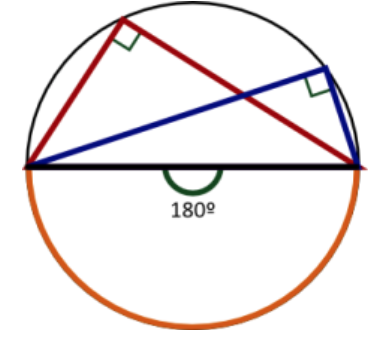
\includegraphics [width=0.34\textwidth ]{img-sol/t9-32} \par La bisectriu de l'angle recte va del vèrtex al punt mitjà de la hipotenusa.
\vspace{0.25cm}
\item[\fontfamily{phv}\selectfont\color{blue}\textbf{32. }] 
L'angle inscrit mesura la meitat que l'angle central. En aquest cas, la meitat de 180 és 90.
\vspace{0.25cm}
\item[\fontfamily{phv}\selectfont\color{blue}\textbf{33. }] 
 Des de qualsevol punt de la circumferència circumscrita al triangle format per el punt de penal i les bases dels pals de la porteria. \par 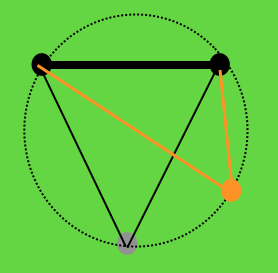
\includegraphics [width=0.35\textwidth ]{img-sol/t9-33}
\vspace{0.25cm}
\item[\fontfamily{phv}\selectfont\color{blue}\textbf{34. }] 
$L=2\pi \cdot 6379 = 40080.44$ km
\vspace{0.25cm}
\item[\fontfamily{phv}\selectfont\color{blue}\textbf{35. }] 
6366 km
 \end{enumerate}
\vspace{0.3cm}

 \needspace{4\baselineskip} 

{\textbf{\em Pàgina 119}} \hrulefill
\begin{enumerate}
\vspace{0.25cm}
\item[\fontfamily{phv}\selectfont\color{blue}\textbf{36. }] 
Aproximadament 14.8 km
 \end{enumerate}
\begin{enumerate}
\vspace{0.25cm}
\item[\fontfamily{phv}\selectfont\color{blue}\textbf{37. }] 
$A=43.3$ cm$^2$
\vspace{0.25cm}
\item[\fontfamily{phv}\selectfont\color{blue}\textbf{38. }] 
$A=254.47$ cm$^2$
\vspace{0.25cm}
\item[\fontfamily{phv}\selectfont\color{blue}\textbf{39. }] 
$A=119\pi =376.85$ cm$^2$
\vspace{0.25cm}
\item[\fontfamily{phv}\selectfont\color{blue}\textbf{40. }] 
Sector: 18.85 cm$^2$ i el segment 3.26 cm$^2$
\vspace{0.25cm}
\item[\fontfamily{phv}\selectfont\color{blue}\textbf{41. }] 
$301\frac {\pi }{6}=157.60$ cm$^2$
\vspace{0.25cm}
\item[\fontfamily{phv}\selectfont\color{blue}\textbf{42. }]  \scalebox{0.6}{\simbolclau } 
$A=10^2-\pi 5^2=21.46$ cm$^2$
\vspace{0.25cm}
\item[\fontfamily{phv}\selectfont\color{blue}\textbf{43. }] 
En general $\frac {R^2}{2}(\pi - \sqrt {3})=1.41$ m$^2$
\vspace{0.25cm}
\item[\fontfamily{phv}\selectfont\color{blue}\textbf{44. }] 
$64\cdot \left (\frac {5\pi }{6} + \frac {\sqrt {3}}{4} \right )=195.26$ cm$^2$
\vspace{0.25cm}
\item[\fontfamily{phv}\selectfont\color{blue}\textbf{45. }] 
$A=\pi \cdot 12^2 - 5 \pi \cdot 4^2=64 \cdot \pi =201.06$ cm$^2$
\vspace{0.25cm}
\item[\fontfamily{phv}\selectfont\color{blue}\textbf{46. }] 
$A=\frac {24\pi }{9}=9.77$ cm$^2$
 \end{enumerate}
\vspace{0.3cm}

 \needspace{4\baselineskip} 

{\textbf{\em Pàgina 120}} \hrulefill
\begin{enumerate}
\vspace{0.25cm}
\item[\fontfamily{phv}\selectfont\color{blue}\textbf{47. }]  \scalebox{0.6}{\simbolclau } 
$A=\frac {9}{2}+ \frac {135}{360} \cdot \pi \cdot 18 = 25.71$ cm$^2$
 \end{enumerate}
\begin{enumerate}
\vspace{0.25cm}
\item[\fontfamily{phv}\selectfont\color{blue}\textbf{48. }] 
$A=9\sqrt {3}-4\pi =3.02$ cm$^2$
\vspace{0.25cm}
\item[\fontfamily{phv}\selectfont\color{blue}\textbf{49. }]  \scalebox{0.6}{\simbolclau } 
$P=62.83$ cm i $A=222.03$ cm$^2$
 \end{enumerate}
\vspace{0.3cm}

 \needspace{4\baselineskip} 

{\textbf{\em Pàgina 121}} \hrulefill
\begin{enumerate}
\vspace{0.25cm}
\item[\fontfamily{phv}\selectfont\color{blue}\textbf{50. }] 
 L'altura corresponent al costat desigual és també mitjana, mediatriu i bisectriu. Les altres rectes notables no coincideixen.
 \end{enumerate}
\begin{enumerate}
\vspace{0.25cm}
\item[\fontfamily{phv}\selectfont\color{blue}\textbf{51. }] 
 Si la posem al circumcentre, els tres vèrtex rebran la mateixa llum, però pot ser molt poca si es tracta d'un triangle obtusangle (el circumcentre quedarà fora de la plaça). Si la posem en l'incentre, tindrem un cercle complet de bona llum dins de la plaça, però no necessàriament en els vèrtexs.
\vspace{0.25cm}
\item[\fontfamily{phv}\selectfont\color{blue}\textbf{52. }] 
Ha recorregut 4 cm
\vspace{0.25cm}
\item[\fontfamily{phv}\selectfont\color{blue}\textbf{53. }] 
En l'incentre
 \end{enumerate}
\vspace{0.3cm}

 \needspace{4\baselineskip} 

{\textbf{\em Pàgina 122}} \hrulefill
\begin{enumerate}
\vspace{0.25cm}
\item[\fontfamily{phv}\selectfont\color{blue}\textbf{54. }] 
Ha de seguir una de les medianes
 \end{enumerate}
\begin{enumerate}
\vspace{0.25cm}


 \needspace{2\baselineskip} 

 \item[\fontfamily{phv}\selectfont\color{blue}\textbf{55}. ] 
 \begin{tasks}[column-sep=1em, item-indent=1.3333em](1)
	 \task*  L'angle central corresponent a un angle inscrit d'90$^\circ $ mesura 180$^\circ $. Per tant la hipotenusa del triangle ha de ser un diàmetre de la circumferència.
	 \task* L'ortocentre es troba en el vèrtex de l'angle recta.
\end{tasks}
\vspace{0.25cm}
\item[\fontfamily{phv}\selectfont\color{blue}\textbf{56. }] 
Solució manipulativa
\vspace{0.25cm}
\item[\fontfamily{phv}\selectfont\color{blue}\textbf{57. }] 
$20\sqrt {3}$ cm
\vspace{0.25cm}
\item[\fontfamily{phv}\selectfont\color{blue}\textbf{58. }] 
Solució manipulativa utilitzant Geogebra
\vspace{0.25cm}
\item[\fontfamily{phv}\selectfont\color{blue}\textbf{59. }] 
Solució manipulativa utilitzant Geogebra: El triangle ha d'ésser isòscels
\vspace{0.25cm}
\item[\fontfamily{phv}\selectfont\color{blue}\textbf{60. }] 
Una circumferència en centre la bomba i radi 50 m.
\vspace{0.25cm}
\item[\fontfamily{phv}\selectfont\color{blue}\textbf{61. }] 
A la mediatriu del segment, els extrems són els dos participants.
\vspace{0.25cm}
\item[\fontfamily{phv}\selectfont\color{blue}\textbf{62. }] 
Ens trobam a igual distància del centre i per tant rebem la mateixa quantitat de calor.
\vspace{0.25cm}
\item[\fontfamily{phv}\selectfont\color{blue}\textbf{63. }] 
Resposta gràfica
\vspace{0.25cm}
\item[\fontfamily{phv}\selectfont\color{blue}\textbf{64. }] 
Resposta gràfica
\vspace{0.25cm}
\item[\fontfamily{phv}\selectfont\color{blue}\textbf{65. }] 
Resposta gràfica i manipulativa
\vspace{0.25cm}
\item[\fontfamily{phv}\selectfont\color{blue}\textbf{66. }] 
Resposta gràfica i manipulativa
\vspace{0.25cm}
\item[\fontfamily{phv}\selectfont\color{blue}\textbf{67. }] 
 Les medianes són també mediatrius, bisectrius i altures. Els quatre punts notables coincideixen.
 \end{enumerate}
\vspace{0.3cm}

 \needspace{4\baselineskip} 

{\textbf{\em Pàgina 123}} \hrulefill
\begin{enumerate}
\vspace{0.25cm}


 \needspace{2\baselineskip} 

 \item[\fontfamily{phv}\selectfont\color{blue}\textbf{68}. ] 
 \begin{tasks}[column-sep=1em, item-indent=1.3333em](2)
	 \task Sí
	 \task Sí
	 \task Sí
	 \task No
\end{tasks}
 \end{enumerate}
\begin{enumerate}
\vspace{0.25cm}


 \needspace{2\baselineskip} 

 \item[\fontfamily{phv}\selectfont\color{blue}\textbf{69}. ] 
 \begin{tasks}[column-sep=1em, item-indent=1.3333em](1)
	 \task* No es pot trobar $c'$ perquè no són semblants $\frac {15}{10}\neq \frac {9}{4}$
	 \task $a'=12$ cm
\end{tasks}
\vspace{0.25cm}
\item[\fontfamily{phv}\selectfont\color{blue}\textbf{70. }] 
27, 31.5 i 31.5 cm
\vspace{0.25cm}
\item[\fontfamily{phv}\selectfont\color{blue}\textbf{71. }] 
Els angles són 36, 72 i 72 graus.
\vspace{0.25cm}
\item[\fontfamily{phv}\selectfont\color{blue}\textbf{72. }] 
L'edifici fa 22.5 m
\vspace{0.25cm}
\item[\fontfamily{phv}\selectfont\color{blue}\textbf{73. }] 
Area ABC=1350; Area ACD=486; CD=36; DE=28.8; EF=23.04
\vspace{0.25cm}
\item[\fontfamily{phv}\selectfont\color{blue}\textbf{74. }] 
Són semblants. El perímetre és la meitat i l'àrea la quarta part.
\vspace{0.25cm}
\item[\fontfamily{phv}\selectfont\color{blue}\textbf{75. }] 
Si els costats són proporcionals, necessàriament les medianes també.
\vspace{0.25cm}
\item[\fontfamily{phv}\selectfont\color{blue}\textbf{76. }] 
24.5 cm$^2$ i 12.25 cm$^2$
\vspace{0.25cm}
\item[\fontfamily{phv}\selectfont\color{blue}\textbf{77. }] 
$2500 \text { cm}{}^2 \cdot \frac {(3\cdot 10^6)^2 \text { cm}{}^2}{1 \text { cm}{}^2}\cdot \frac {1 \text { km}{}^2}{10^{10} \text { cm}{}^2} = 2.25 \cdot 10^6 \text { km}^2$
\vspace{0.25cm}
\item[\fontfamily{phv}\selectfont\color{blue}\textbf{78. }] 
L'altura $\frac {104}{7}=14.86$ cm; Les àrees són: 14 cm$^2$ i 193.14 cm$^2$
 \end{enumerate}
\vspace{0.3cm}

 \needspace{4\baselineskip} 

{\textbf{\em Pàgina 124}} \hrulefill
\begin{enumerate}
\vspace{0.25cm}
\item[\fontfamily{phv}\selectfont\color{blue}\textbf{79. }] 
Per semblança $\frac {0.05}{R}=\frac {1}{1 500 000}$, $R=750 000$ km. El diàmetre del Sol és 1.5 milions de km.
 \end{enumerate}
\begin{enumerate}
\vspace{0.25cm}


 \needspace{2\baselineskip} 

 \item[\fontfamily{phv}\selectfont\color{blue}\textbf{80}. ] 
 \begin{tasks}[column-sep=1em, item-indent=1.3333em](2)
	 \task $\alpha = 180 - (A+180-B)=B-A$
	 \task* $2A+2\alpha =360$; $\alpha =180-A$
\end{tasks}
\vspace{0.25cm}
\item[\fontfamily{phv}\selectfont\color{blue}\textbf{81. }] 
El costat fa 3.8 cm
\vspace{0.25cm}
\item[\fontfamily{phv}\selectfont\color{blue}\textbf{82. }] 
$a_p=\frac {7}{2}\sqrt {3}=6.1$ cm
\vspace{0.25cm}
\item[\fontfamily{phv}\selectfont\color{blue}\textbf{83. }] 
$A=\frac {25^2}{\pi }=198.94$ cm$^2$
\vspace{0.25cm}
\item[\fontfamily{phv}\selectfont\color{blue}\textbf{84. }] 
$L=10\sqrt {2\pi }=25.1$ cm$^2$
\vspace{0.25cm}
\item[\fontfamily{phv}\selectfont\color{blue}\textbf{85. }] 
L'equador fa 40000 km; La velocitat $v=50 000/3$ km/h
\vspace{0.25cm}
\item[\fontfamily{phv}\selectfont\color{blue}\textbf{86. }] 
Si el triangle és equilàter $\frac {3\sqrt {3}}{4\pi }$; sinó falten dades.
\vspace{0.25cm}
\item[\fontfamily{phv}\selectfont\color{blue}\textbf{87. }] 
$c=23/6$
\vspace{0.25cm}
\item[\fontfamily{phv}\selectfont\color{blue}\textbf{88. }] 
Necessita $4908.74$ kg. Aprox. 5 tones.
\vspace{0.25cm}
\item[\fontfamily{phv}\selectfont\color{blue}\textbf{89. }] 
Arriba a una altura de 3.71 m
\vspace{0.25cm}
\item[\fontfamily{phv}\selectfont\color{blue}\textbf{90. }] 
$A=102.1$ cm$^2$
\vspace{0.25cm}
\item[\fontfamily{phv}\selectfont\color{blue}\textbf{91. }] 
Hexàgon: 23.38 cm$^2$; Hexàgon estrellat: 46.77 cm$^2$
\vspace{0.25cm}
\item[\fontfamily{phv}\selectfont\color{blue}\textbf{92. }] 
Aprox. 6600 cm$^2$
\vspace{0.25cm}
\item[\fontfamily{phv}\selectfont\color{blue}\textbf{93. }] 
$\left . \begin {array}{l} 25^2=x^2+h^2 \\ 17^2 =(28-x)^2+h^2 \end {array} \right \}$ \par $x=20$ m i $h=15$ m. L'àrea és $A=390$ m$^2$.
\vspace{0.25cm}
\item[\fontfamily{phv}\selectfont\color{blue}\textbf{94. }] 
43.30 cm$^2$
\vspace{0.25cm}
\item[\fontfamily{phv}\selectfont\color{blue}\textbf{95. }] 
259.81 cm$^2$
\vspace{0.25cm}
\item[\fontfamily{phv}\selectfont\color{blue}\textbf{96. }] 
Aquesta figura és impossible ja que l'altura 4 és major que el costat 3. Queda un triangle rectangle on la hipotenusa mesuraria menys que un catet.
\vspace{0.25cm}
\item[\fontfamily{phv}\selectfont\color{blue}\textbf{97. }] 
$A=19.80$ cm$^2$
\vspace{0.25cm}
\item[\fontfamily{phv}\selectfont\color{blue}\textbf{98. }] 
$A=29.98$ cm$^2$ i $P=19.49$ cm
 \end{enumerate}
\vspace{0.3cm}

 \needspace{4\baselineskip} 

{\textbf{\em Pàgina 125}} \hrulefill
\begin{enumerate}
\vspace{0.25cm}
\item[\fontfamily{phv}\selectfont\color{blue}\textbf{99. }] 
$A=40.5$ cm$^2$ i $P=25.46$ cm
 \end{enumerate}
\begin{enumerate}
\vspace{0.25cm}
\item[\fontfamily{phv}\selectfont\color{blue}\textbf{100. }] 
$A=24$ cm$^2$ i $P=22.42$ cm
\vspace{0.25cm}
\item[\fontfamily{phv}\selectfont\color{blue}\textbf{101. }] 
Estrictament no. Si suposam que $\pi =3$ i que la base i l'altura són els catets, llavors sí.
\vspace{0.25cm}
\item[\fontfamily{phv}\selectfont\color{blue}\textbf{102. }] 
$\sqrt {2}$, $\sqrt {3}$, $\sqrt {4}=2$, $\sqrt {5}$, $\sqrt {6}$
\vspace{0.25cm}
\item[\fontfamily{phv}\selectfont\color{blue}\textbf{103. }] 
$\sqrt {5}$, $\sqrt {6}$ i $\sqrt {7}$ cm
\vspace{0.25cm}
\item[\fontfamily{phv}\selectfont\color{blue}\textbf{104. }] 
$H=5\sqrt {7}=13.23$ cm$^2$
\vspace{0.25cm}
\item[\fontfamily{phv}\selectfont\color{blue}\textbf{105. }] 
$g=\sqrt {74}=8.602$ m
\vspace{0.25cm}
\item[\fontfamily{phv}\selectfont\color{blue}\textbf{106. }] 
$-10+10\sqrt {41}=54.03$ m
\vspace{0.25cm}
\item[\fontfamily{phv}\selectfont\color{blue}\textbf{107. }] 
$x=211.681$
 \end{enumerate}
\vspace{0.3cm}

 \needspace{4\baselineskip} 

{\textbf{\em Pàgina 126}} \hrulefill
\begin{enumerate}
\vspace{0.25cm}
 \item[$\bullet$ ] {\fontfamily{phv}\selectfont\color{blue}\textbf{Autoavaluació:}. }

 \end{enumerate}
\begin{enumerate}
\vspace{0.25cm}
\item[\fontfamily{phv}\selectfont\color{blue}\textbf{1. }]  \scalebox{0.6}{\simbolclau } 
\textbf {--10.} Autoavaluació: 1d; 2b; 3c; 4a; 5d; 6a; 7a; 8c; 9d; 10a
 \end{enumerate}
\vfill\null
\columnbreak
\def\currentname{Solucions del Tema 10}
\vspace*{0.75cm}

 
 \needspace{5\baselineskip} 
 \scalebox{1.25}{\heading{Solucions del Tema 10}}

\vspace*{0.4cm}
\phantomsection \addcontentsline{toc}{section}{Solucions del Tema 10}
\vspace{0.3cm}

 \needspace{4\baselineskip} 

{\textbf{\em Pàgina 128}} \hrulefill
\begin{enumerate}
\vspace{0.25cm}


 \needspace{2\baselineskip} 

 \item[$\bullet$ ] {\fontfamily{phv}\selectfont\color{blue}\textbf{Avaluació inicial}. } 
 \begin{tasks}[column-sep=1em, item-indent=1.3333em](1)
	 \task Translació
	 \task Homotècia
	 \task Simetria axial
	 \task Simetria central
	 \task Rotació
	 \task* Rotació de $270^\circ $ + simetria axial
\end{tasks}
 \end{enumerate}
\vspace{0.3cm}

 \needspace{4\baselineskip} 

{\textbf{\em Pàgina 129}} \hrulefill
\begin{enumerate}
\vspace{0.25cm}
\item[\fontfamily{phv}\selectfont\color{blue}\textbf{1. }] 
Gràfica:\par 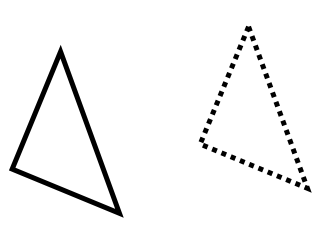
\includegraphics [width=0.34\textwidth ]{img-sol/t10-1}\par Hem fet una translació: Tots els costats i tots els angles mesuren el mateix que el triangle original. 
 \end{enumerate}
\begin{enumerate}
\vspace{0.25cm}
\item[\fontfamily{phv}\selectfont\color{blue}\textbf{2. }] 
Gràfica:\par 
\includegraphics [width=0.34\textwidth ]{img-sol/t10-2}
\vspace{0.25cm}
\item[\fontfamily{phv}\selectfont\color{blue}\textbf{3. }] 
Els costats són el doble de grans i els angles són iguals. És una semblança de raó 2:\par 
\includegraphics [width=0.4\textwidth ]{img-sol/t10-3}
\vspace{0.25cm}
\item[\fontfamily{phv}\selectfont\color{blue}\textbf{4. }] 
La lletra \textbf {d} minúscula és una simetria especular de la \textbf {b} anterior.
\vspace{0.25cm}
\item[\fontfamily{phv}\selectfont\color{blue}\textbf{5. }] 
Gràfica:\par 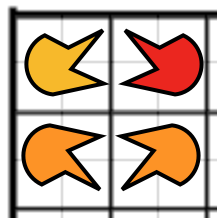
\includegraphics [width=0.34\textwidth ]{img-sol/t10-5}
\vspace{0.25cm}
\item[\fontfamily{phv}\selectfont\color{blue}\textbf{6. }] 
Gràfica:\par 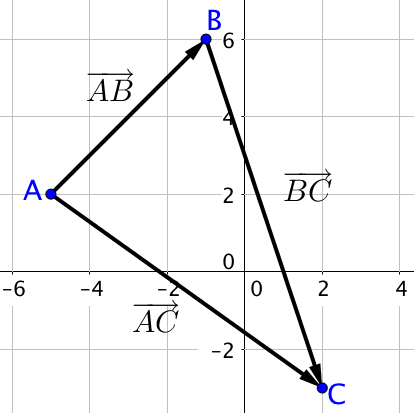
\includegraphics [width=0.34\textwidth ]{img-sol/t10-6}\par $\overrightarrow {AB}=B-A=(4, 4)$, $\overrightarrow {AC}=C-A=(7, -5)$, $\overrightarrow {BC}=C-B=(3,-9)$, $\overrightarrow {CA}=A-C=(-7,5)$ i $\overrightarrow {CB}=B-C=(-3,9)$
\vspace{0.25cm}
\item[\fontfamily{phv}\selectfont\color{blue}\textbf{7. }] 
Gràfica:\par 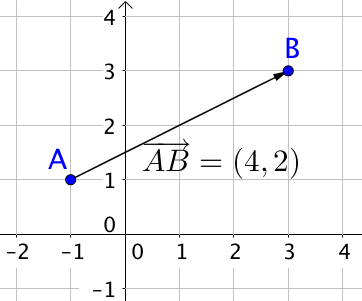
\includegraphics [width=0.34\textwidth ]{img-sol/t10-7}\par $\overrightarrow {AB}=B-A$ $\rightarrow $, $(4,2)=B-(-1,1)$ del qual aïllam $B=(4,2)+(-1,1)=(3,3)$.
\vspace{0.25cm}
\item[\fontfamily{phv}\selectfont\color{blue}\textbf{8. }] 
$\vec a =(1,1)$; $\vec b=(0,-3)$; $\vec u=(3,1)$; $\vec v=(3,1)$; $\vec w=(1,-3)$. Els vectors $\vec u$ i $\vec v$ són representats del mateix vector lliure.
 \end{enumerate}
\vspace{0.3cm}

 \needspace{4\baselineskip} 

{\textbf{\em Pàgina 130}} \hrulefill
\begin{enumerate}
\vspace{0.25cm}
\item[\fontfamily{phv}\selectfont\color{blue}\textbf{9. }] 
Gràfica:\par 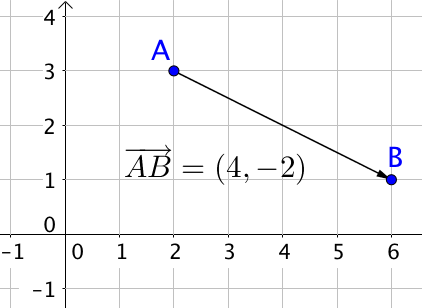
\includegraphics [width=0.34\textwidth ]{img-sol/t10-9}\par $\overrightarrow {AB}=B-A$ $\rightarrow $, $(4,-2)=B-(2,3)$ del qual aïllam $B=(4,-2)+(2,3)=(6,1)$.
 \end{enumerate}
\begin{enumerate}
\vspace{0.25cm}
\item[\fontfamily{phv}\selectfont\color{blue}\textbf{10. }] 
Solució gràfica:\par 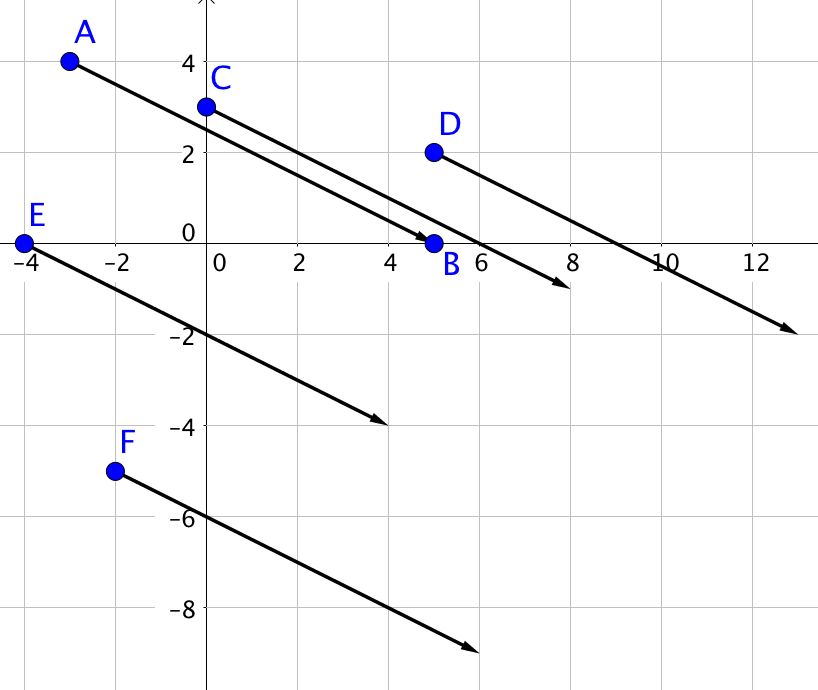
\includegraphics [width=0.4\textwidth ]{img-sol/t10-equipolent}
\vspace{0.25cm}
\item[\fontfamily{phv}\selectfont\color{blue}\textbf{12. }] 
$\overrightarrow {DE}=D-E=(-4,-2)$ i $\overrightarrow {FG}=G-F=(-4,-2)$ són equipol·lents. Sí. Són representants d'un mateix vector lliure.
\vspace{0.25cm}


 \needspace{2\baselineskip} 

 \item[\fontfamily{phv}\selectfont\color{blue}\textbf{13}. ] 
 \begin{tasks}[column-sep=1em, item-indent=1.3333em](1)
	 \task $\vec u = (-9,-11)$
	 \task $\vec v=(7,-11)$
	 \task $\vec w=(-2,-10)$
\end{tasks}
\vspace{0.25cm}


 \needspace{2\baselineskip} 

 \item[\fontfamily{phv}\selectfont\color{blue}\textbf{14}. ]  \scalebox{0.6}{\simbolclau } 
 \begin{tasks}[column-sep=1em, item-indent=1.3333em](1)
	 \task $(-17,15)$
	 \task $(23,-7)$
	 \task $(-11,-14)$
\end{tasks}
 \end{enumerate}
\vspace{0.3cm}

 \needspace{4\baselineskip} 

{\textbf{\em Pàgina 131}} \hrulefill
\begin{enumerate}
\vspace{0.25cm}
\item[\fontfamily{phv}\selectfont\color{blue}\textbf{15. }] 
El vector $\vec u + \vec v = (6,2)$. Si el dibuixam en origen el punt $A(1,2)$, aleshores el vector suma té extrem en el punt $B(7,4)$
 \end{enumerate}
\begin{enumerate}
\vspace{0.25cm}


 \needspace{2\baselineskip} 

 \item[\fontfamily{phv}\selectfont\color{blue}\textbf{16}. ] 
 \begin{tasks}[column-sep=1em, item-indent=1.3333em](2)
	 \task $(3,-6)$
	 \task $(3,\frac {3}{2})$
	 \task $(65,-99)$
	 \task $(22.3,61)$
\end{tasks}
\vspace{0.25cm}
\item[\fontfamily{phv}\selectfont\color{blue}\textbf{18. }] 
Les dues figures tenen totes les seves longituds i angles iguals. Aquestes rectes són paral·leles. Han seguit un vector lliure.
\vspace{0.25cm}
\item[\fontfamily{phv}\selectfont\color{blue}\textbf{19. }]  \scalebox{0.6}{\simbolclau } 
És una translació de vector $\vec t_1 + \vec t_2 = (-1,-1)$
\vspace{0.25cm}
\item[\fontfamily{phv}\selectfont\color{blue}\textbf{21. }] 
$A’ = (7, 3)$; $B’ = (7, 5)$; $C’ = (5, 5)$
\vspace{0.25cm}
\item[\fontfamily{phv}\selectfont\color{blue}\textbf{22. }] 
Gràfica:\par 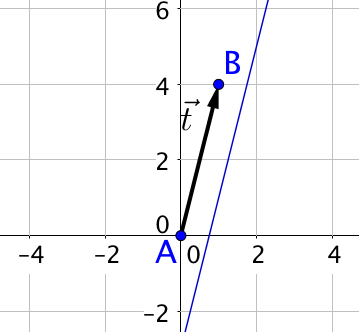
\includegraphics [width=0.35\textwidth ]{img-sol/t10-23}
 \end{enumerate}
\vspace{0.3cm}

 \needspace{4\baselineskip} 

{\textbf{\em Pàgina 132}} \hrulefill
\begin{enumerate}
\vspace{0.25cm}
\item[\fontfamily{phv}\selectfont\color{blue}\textbf{25. }]  \scalebox{0.6}{\simbolclau } 
\textit {A'} (2, 4), \textit {B'} ($-$2, 3) i \textit {C'} (0, 5)
 \end{enumerate}
\begin{enumerate}
\vspace{0.25cm}
\item[\fontfamily{phv}\selectfont\color{blue}\textbf{26. }] 
 Mitjançant el gir la recta es transforma en una recta, la circumferència, el segment i el triangle en una circumferència, un segment i un triangle igual, respectivament. Dues rectes paral·leles en dos rectes paral·leles, i dues rectes perpendiculars, en dues rectes perpendiculars.
\vspace{0.25cm}
\item[\fontfamily{phv}\selectfont\color{blue}\textbf{28. }]  \scalebox{0.6}{\simbolclau } 
 Un gir de $60^\circ $ no deixa cap recta invariant. Un gir de $180^\circ $ deixa invariants les rectes que passen del centre de gir. Les rotacions de $0^\circ $ i $360^\circ $ són la identitat, deixen la figura original. 
\vspace{0.25cm}
\item[\fontfamily{phv}\selectfont\color{blue}\textbf{29. }] 
Recorda que la simetria central en el pla és un gir de 180$^\circ $, llavors és un moviment directe. Els costats i els angles d'un triangle i el seu girat 180 són iguals, i amb el mateix sentit.
\vspace{0.25cm}
\item[\fontfamily{phv}\selectfont\color{blue}\textbf{30. }] 
No tenen simetria central: B, P, T. Si la tenen: H, N, O, S, X, Z.
\vspace{0.25cm}
\item[\fontfamily{phv}\selectfont\color{blue}\textbf{31. }] 
El pla es transforma en un pla, una esfera en una esfera igual, un con en un altre con igual, els plans paral·lels es transformen en plans paral·lels i els ortogonals en plans ortogonals. 
 \end{enumerate}
\vspace{0.3cm}

 \needspace{4\baselineskip} 

{\textbf{\em Pàgina 133}} \hrulefill
\begin{enumerate}
\vspace{0.25cm}
\item[\fontfamily{phv}\selectfont\color{blue}\textbf{32. }] 
A forma d'exemple:\par 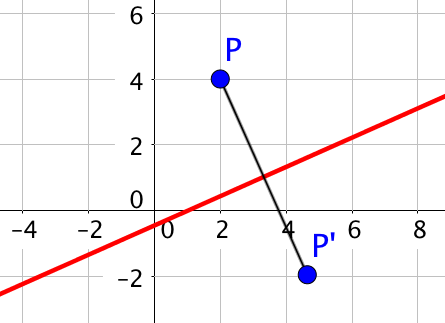
\includegraphics [width=0.35\textwidth ]{img-sol/t10-33}
 \end{enumerate}
\begin{enumerate}
\vspace{0.25cm}
\item[\fontfamily{phv}\selectfont\color{blue}\textbf{33. }] 
L'eix de simetria és la mediatriu del segment $\overline {PP'}$
\vspace{0.25cm}
\item[\fontfamily{phv}\selectfont\color{blue}\textbf{35. }] 
A forma d'exemple:\par 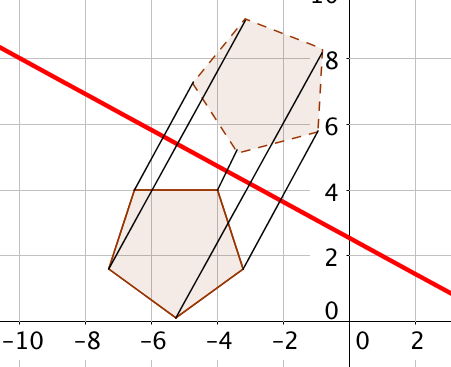
\includegraphics [width=0.35\textwidth ]{img-sol/t10-36}
\vspace{0.25cm}
\item[\fontfamily{phv}\selectfont\color{blue}\textbf{36. }]  \scalebox{0.6}{\simbolclau } 
i) $A'(-3,-4)$, $B'(-5,6)$ i $C'(4,5)$;\par ii) $A'(3,4)$, $B'(5,-6)$ i $C'(-4,-5)$
\vspace{0.25cm}
\item[\fontfamily{phv}\selectfont\color{blue}\textbf{37. }] 
a, b) Solució gràfica:\par 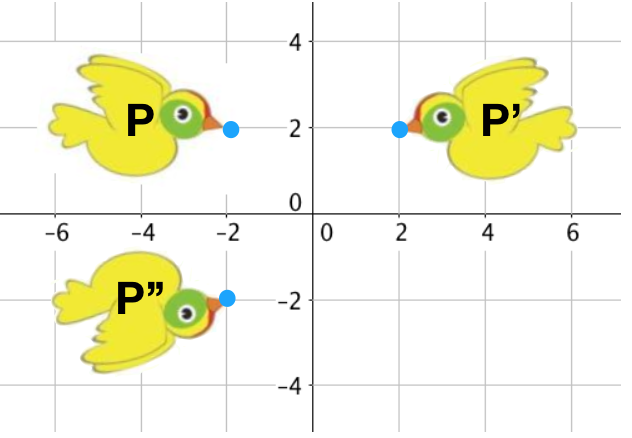
\includegraphics [width=0.35\textwidth ]{img-sol/t10-38}\par c) No existeix cap simetria aixal. Sí. Una simetria central en centre l'origen. \par d) $P'(2,2)$ i $P''(-2,-2)$
 \end{enumerate}
\vspace{0.3cm}

 \needspace{4\baselineskip} 

{\textbf{\em Pàgina 134}} \hrulefill
\begin{enumerate}
\vspace{0.25cm}
\item[\fontfamily{phv}\selectfont\color{blue}\textbf{38. }] 
Eix de simetria horitzontal: B, D. Eix de simetria vertical: A, M, T, U, V, W.
 \end{enumerate}
\begin{enumerate}
\vspace{0.25cm}
\item[\fontfamily{phv}\selectfont\color{blue}\textbf{39. }] 
Mitjançant una simetria la recta es transforma en una recta, la circumferència, el segment i el triangle en una circumferència, un segment i un triangle igual, respectivament. dos rectes paral·leles a dues rectes paral·leles, i dues rectes perpendiculars, en dues rectes perpendiculars.
\vspace{0.25cm}
\item[\fontfamily{phv}\selectfont\color{blue}\textbf{40. }] 
 El rectangle té dos eixos de simetria, les mediatrius dels segments AB i BC
\vspace{0.25cm}
\item[\fontfamily{phv}\selectfont\color{blue}\textbf{41. }] 
 L'hexàgon té 6 eixos de simetria, 3 van de vèrtex a vèrtex oposat, i 3 van de centre de costat a centre de costat oposat.\par El pentàgon té 5 eixos de simetria, que van de vèrtex al centre del costat oposat.
\vspace{0.25cm}
\item[\fontfamily{phv}\selectfont\color{blue}\textbf{42. }] 
El vector de translació és perpendicular a la direcció de les rectes, de sentit de la primera recta a la segona i de mòdul, el doble de la distància entre les rectes.
\vspace{0.25cm}
\item[\fontfamily{phv}\selectfont\color{blue}\textbf{43. }] 
El centre de gir és el punt d'intersecció de les rectes, i l'angle de gir té d'amplitud el doble de l'angle que formen les rectes i de sentit, de la primera recta a la segona.
\vspace{0.25cm}
\item[\fontfamily{phv}\selectfont\color{blue}\textbf{44. }] 
La mateixa simetria. Les simetries són involutives, és a dir $S \circ S=$Identitat.
\vspace{0.25cm}
\item[\fontfamily{phv}\selectfont\color{blue}\textbf{45. }] 
Cal que els eixos siguin ortogonals
\vspace{0.25cm}
\item[\fontfamily{phv}\selectfont\color{blue}\textbf{46. }] 
 Per exemple: la meva cadira, la taula, el meu ordinador, el llum, un llapis.
\vspace{0.25cm}


 \needspace{2\baselineskip} 

 \item[\fontfamily{phv}\selectfont\color{blue}\textbf{47}. ] 
 \begin{tasks}[column-sep=1em, item-indent=1.3333em](1)
	 \task* Té 5 plans de simetria; 2 passen per 4 vèrtexs i 2 arestes laterals; 2 passen pels punts mitjans de 4 arestes de la base; 1 passa pels punts mitjans de les arestes laterals. Té un eix de rotació de 90$^\circ $
	 \task* 180$^\circ $ i 270$^\circ $ que va de centre de la base quadrada a centre de l'altra base. \par Si és unn prisma oblic; no en té cap.
	 \task* Piràmide de base quadrada té 4 plans de simetria; 2 passen per 2 vèrtexs de la base i el vèrtex i els altres 2; pels punts mitjans de les arestes de la base i el vèrtex. Té un eix de rotació de 90$^\circ $
	 \task* 180$^\circ $ i 270$^\circ $ que passa pel vèrtex i el centre de quadrat de la base
	 \task* Es perden els plans de simetria que passen per dues arestes. 
\end{tasks}
\vspace{0.25cm}


 \needspace{2\baselineskip} 

 \item[\fontfamily{phv}\selectfont\color{blue}\textbf{48}. ] 
 \begin{tasks}[column-sep=1em, item-indent=1.3333em](1)
	 \task* 3 Plans que passin per una aresta i la meitat d'una cara rectangular; 1 pla que passi per la meitat de les arestes laterals
	 \task* 3 Plans que passin per una aresta i la meitat d'una cara lateral; Si és oblic no té cap pla de simetria
	 \task* 1 pla que divideixi la base en dos triangles iguals i 1 pla que passi per la meitat de les arestes laterals
\end{tasks}
\vspace{0.25cm}
\item[\fontfamily{phv}\selectfont\color{blue}\textbf{49. }] 
El pla es transforma en un pla, una esfera en una esfera igual, un con en un altre con igual, els plans paral·lels es transformen en plans paral·lels i els ortogonals en plans ortogonals.
\vspace{0.25cm}
\item[\fontfamily{phv}\selectfont\color{blue}\textbf{50. }] 
Els punts sobre l'eix de simetria. Rectes invariants, a més de l'eix, que és una recta invariant de punts invariants, són rectes invariants les rectes ortogonals a l'eix de simetria.
 \end{enumerate}
\vspace{0.3cm}

 \needspace{4\baselineskip} 

{\textbf{\em Pàgina 136}} \hrulefill
\begin{enumerate}
\vspace{0.25cm}
\item[\fontfamily{phv}\selectfont\color{blue}\textbf{60. }] 
Respecte l'estrella \textbf {*}, les fulles s'obtenen per simetria central. També \textbf {*} és el centre de gir de les fulles negres d'amplitud 180$^\circ $. Si no tenim en compte el color de les fulles, també tenim simetria de gir d'amplitud $360/12=30^\circ $
 \end{enumerate}
\begin{enumerate}
\vspace{0.25cm}


 \needspace{2\baselineskip} 

 \item[\fontfamily{phv}\selectfont\color{blue}\textbf{61}. ] 
 \begin{tasks}[column-sep=1em, item-indent=1.3333em](1)
	 \task  En L4 i L5
	 \task L2 i L5
	 \task L3; L5 i L7
	 \task Sí; en L6 i L7
	 \task* Translació; simetria horitzontal; simetria vertical; gir de 180$^\circ $ i simetria amb lliscament.
\end{tasks}
 \end{enumerate}
\vspace{0.3cm}

 \needspace{4\baselineskip} 

{\textbf{\em Pàgina 137}} \hrulefill
\begin{enumerate}
\vspace{0.25cm}
\item[\fontfamily{phv}\selectfont\color{blue}\textbf{63. }] 
En aquests frisos s'han utilitzat: Translació, simetria horitzontal, simetria vertical, gir de 180$^\circ $, i simetria amb lliscament.\par a) en el primer únicament hi ha translació \par b) girs de 180$^\circ $; \par c) simetria d'eix vertical\par d) Simetria d'eix horitzontal \par e) simetries d'eix horitzontal i d'eix vertical, i per tant girs de 180$^\circ $
 \end{enumerate}
\begin{enumerate}
\vspace{0.25cm}


 \needspace{2\baselineskip} 

 \item[\fontfamily{phv}\selectfont\color{blue}\textbf{64}. ] 
 \begin{tasks}[column-sep=1em, item-indent=1.3333em](1)
	 \task Té simetria central 2; 3 i 5
	 \task* Tenen simetria axial tots excepte el 4.
	 \task Tots tenen centre de gir
	 \task Solució oberta
\end{tasks}
 \end{enumerate}
\vspace{0.3cm}

 \needspace{4\baselineskip} 

{\textbf{\em Pàgina 138}} \hrulefill
\begin{enumerate}
\vspace{0.25cm}
 \item[$\bullet$ ] {\fontfamily{phv}\selectfont\color{blue}\textbf{Autoavaluació:}. }

 \end{enumerate}
\begin{enumerate}
\vspace{0.25cm}
\item[\fontfamily{phv}\selectfont\color{blue}\textbf{1. }]  \scalebox{0.6}{\simbolclau } 
\textbf {--10. } Autoavaluació: 1b; 2c; 3b; 4d; 5c; 6b; 7b; 8b; 9d; 10b;
 \end{enumerate}
\vfill\null
\columnbreak
\def\currentname{Solucions del Tema 11}
\vspace*{0.75cm}

 
 \needspace{5\baselineskip} 
 \scalebox{1.25}{\heading{Solucions del Tema 11}}

\vspace*{0.4cm}
\phantomsection \addcontentsline{toc}{section}{Solucions del Tema 11}
\vspace{0.3cm}

 \needspace{4\baselineskip} 

{\textbf{\em Pàgina 140}} \hrulefill
\begin{enumerate}
\vspace{0.25cm}


 \needspace{2\baselineskip} 

 \item[\fontfamily{phv}\selectfont\color{blue}\textbf{1}. ] 
 \begin{tasks}[column-sep=1em, item-indent=1.3333em](1)
	 \task* El terra i el sòtil són plans paral·lels. El terra i una paret són plans perpendiculars
	 \task* El rodapeus de cada banda de classe són rectes paral·leles
	 \task etc.
\end{tasks}
 \end{enumerate}
\begin{enumerate}
\vspace{0.25cm}
\item[\fontfamily{phv}\selectfont\color{blue}\textbf{2. }] 
Angle de 72$^\circ $
\vspace{0.25cm}
\item[\fontfamily{phv}\selectfont\color{blue}\textbf{3. }] 
Angle de 60$^\circ $
\vspace{0.25cm}
\item[\fontfamily{phv}\selectfont\color{blue}\textbf{4. }] 
Han d'ésser iguals els tres diedres que el formen.
 \end{enumerate}
\vspace{0.3cm}

 \needspace{4\baselineskip} 

{\textbf{\em Pàgina 141}} \hrulefill
\begin{enumerate}
\vspace{0.25cm}


 \needspace{2\baselineskip} 

 \item[\fontfamily{phv}\selectfont\color{blue}\textbf{5}. ] 
 \begin{tasks}[column-sep=1em, item-indent=1.3333em](1)
	 \task* Poliedre. No convex. $C=7$; $V=10$; $A=15$. Euler $7+10 = 15+2$
	 \task* Poliedre. Convex. $C=8$; $V=12$; $A=18$. Sí Euler $8+12=18+2$
	 \task No Poliedre.
	 \task* Poliedre. Convex. $C=13$; $V=14$; $A=25$. Sí Euler $13+14=25+2$
	 \task* Poliedre. No convex. $C=10$; $V=16$; $A=24$. Euler $10+16=24+2$
\end{tasks}
 \end{enumerate}
\vspace{0.3cm}

 \needspace{4\baselineskip} 

{\textbf{\em Pàgina 142}} \hrulefill
\begin{enumerate}
\vspace{0.25cm}
\item[\fontfamily{phv}\selectfont\color{blue}\textbf{6. }] 
No. Si les bases són dos rectangles iguals i les cares laterals són romboides es tracta d'un prisma oblic.
 \end{enumerate}
\begin{enumerate}
\vspace{0.25cm}
\item[\fontfamily{phv}\selectfont\color{blue}\textbf{7. }] 
 Té set cares, quinze arestes i deu vèrtexs: 7 + 10 = 15 + 2.
\vspace{0.25cm}


 \needspace{2\baselineskip} 

 \item[\fontfamily{phv}\selectfont\color{blue}\textbf{8}. ] 
 \begin{tasks}[column-sep=1em, item-indent=1.3333em](2)
	 \task Irregular
	 \task Regular
	 \task Regular
	 \task Irregular
	 \task Irregular
\end{tasks}
\vspace{0.25cm}
\item[\fontfamily{phv}\selectfont\color{blue}\textbf{9. }] 
Resposta gràfica:\par 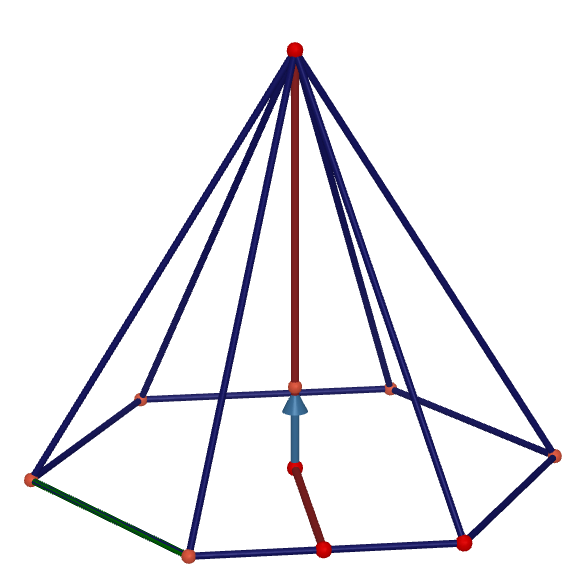
\includegraphics [width=0.4\textwidth ]{img-sol/t11-14a}\par 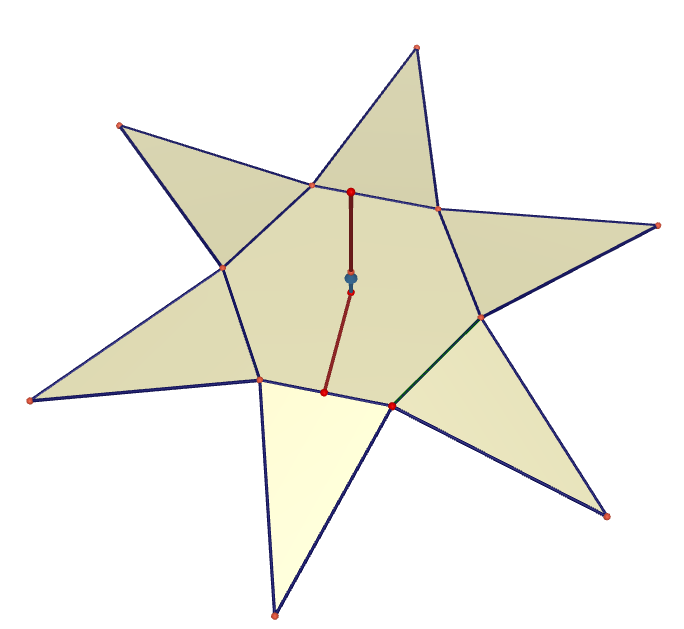
\includegraphics [width=0.4\textwidth ]{img-sol/t11-14b}
\vspace{0.25cm}
\item[\fontfamily{phv}\selectfont\color{blue}\textbf{10. }]  \scalebox{0.6}{\simbolclau } 
Teorema de Pitàgores a l'espai:\par $D=\sqrt {2^2+2^2+2^2}=3.46$ dm
\vspace{0.25cm}
\item[\fontfamily{phv}\selectfont\color{blue}\textbf{11. }]  \scalebox{0.6}{\simbolclau } 
Teorema de Pitàgores a l'espai:\par $D=\sqrt {10^2+4^2+3^2}=11.18$ m
\vspace{0.25cm}
\item[\fontfamily{phv}\selectfont\color{blue}\textbf{12. }] 
\textbf {Atenció} 8 m = 800 cm!\par $A=4800 + 2 \sqrt {3}$ cm$^2 = 4803,4641$ cm$^2$
\vspace{0.25cm}
\item[\fontfamily{phv}\selectfont\color{blue}\textbf{13. }] 
El perímetre de la base són 9 m
\vspace{0.25cm}
\item[\fontfamily{phv}\selectfont\color{blue}\textbf{14. }] 
Apotema = $\sqrt {127}\approx 11,13$ cm; i Àrea = $18 \sqrt {127}+ 108\sqrt {3} \approx 389,91$ cm$^2$.
\vspace{0.25cm}
\item[\fontfamily{phv}\selectfont\color{blue}\textbf{15. }]  \scalebox{0.6}{\simbolclau } 
$A_L=352$ cm$^2$
\vspace{0.25cm}
\item[\fontfamily{phv}\selectfont\color{blue}\textbf{16. }]  \scalebox{0.6}{\simbolclau } 
Totes les arestes mesuren $x=7.75$, l'altura d'una cara lateral $a_P=6.71$ i l'altura de la piràmide $H=5.48$ cm
 \end{enumerate}
\vspace{0.3cm}

 \needspace{4\baselineskip} 

{\textbf{\em Pàgina 143}} \hrulefill
\begin{enumerate}
\vspace{0.25cm}
\item[\fontfamily{phv}\selectfont\color{blue}\textbf{17. }] 
$A_L=\frac {76}{25}\pi \approx 9.550442$ m$^2$
 \end{enumerate}
\begin{enumerate}
\vspace{0.25cm}
\item[\fontfamily{phv}\selectfont\color{blue}\textbf{18. }] 
$A_T = 2016 \pi \approx 63510.44$ cm$^2$
\vspace{0.25cm}
\item[\fontfamily{phv}\selectfont\color{blue}\textbf{19. }]  \scalebox{0.6}{\simbolclau } 
$A_L=4712.4$ dm$^2$
\vspace{0.25cm}
\item[\fontfamily{phv}\selectfont\color{blue}\textbf{20. }] 
$A_T=\left ( \frac {625}{64 \pi } + 25 \right ) \approx 28.108495$ m$^2$
\vspace{0.25cm}


 \needspace{2\baselineskip} 

 \item[\fontfamily{phv}\selectfont\color{blue}\textbf{21}. ] 
 \begin{tasks}[column-sep=1em, item-indent=1.3333em](2)
	 \task $L=8\pi =25.133$ m
	 \task $64\pi =201.062$ m$^2$
\end{tasks}
\vspace{0.25cm}
\item[\fontfamily{phv}\selectfont\color{blue}\textbf{22. }] 
$V=288\sqrt {3}=408.83$ dm$^3$
\vspace{0.25cm}
\item[\fontfamily{phv}\selectfont\color{blue}\textbf{23. }] 
$V=360\pi =1130.97$ cm$^3$. En capacitat $1$ dm$^3$=1 l, llavors aprox. 1,13 litres.
\vspace{0.25cm}


 \needspace{2\baselineskip} 

 \item[\fontfamily{phv}\selectfont\color{blue}\textbf{24}. ]  \scalebox{0.6}{\simbolclau } 
 \begin{tasks}[column-sep=1em, item-indent=1.3333em](2)
	 \task* $V=1000\pi =3140$ dm$^3$=litres
	 \task costarà 2400 \euro {}
\end{tasks}
\vspace{0.25cm}
\item[\fontfamily{phv}\selectfont\color{blue}\textbf{25. }] 
Els dos volums són iguals a $\frac {500 \pi }{3}=523.6$ dm$^3$
 \end{enumerate}
\vspace{0.3cm}

 \needspace{4\baselineskip} 

{\textbf{\em Pàgina 144}} \hrulefill
\begin{enumerate}
\vspace{0.25cm}
\item[\fontfamily{phv}\selectfont\color{blue}\textbf{26. }] 
$0^\circ $ de latitud i $170^\circ $ Oest
 \end{enumerate}
\begin{enumerate}
\vspace{0.25cm}
\item[\fontfamily{phv}\selectfont\color{blue}\textbf{27. }] 
En el pol nord exactament
\vspace{0.25cm}
\item[\fontfamily{phv}\selectfont\color{blue}\textbf{28. }] 
El paral·lel major és l'equador. Tots els meridians són iguals (si menyspream el fet que la Terra no sigui perfectament esfèrica; clar).
\vspace{0.25cm}
\item[\fontfamily{phv}\selectfont\color{blue}\textbf{29. }] 
Binissalem: Latitud=39.688035${}^\circ $ Nord; Longitud=2.8439975${}^\circ $ Est
\vspace{0.25cm}
\item[\fontfamily{phv}\selectfont\color{blue}\textbf{30. }] 
Dotze diedres si l'habitació té sòtil. 8 sense sòtil.
\vspace{0.25cm}
\item[\fontfamily{phv}\selectfont\color{blue}\textbf{31. }] 
Solució oberta i manipulativa
\vspace{0.25cm}
\item[\fontfamily{phv}\selectfont\color{blue}\textbf{32. }] 
135$^\circ $
\vspace{0.25cm}
\item[\fontfamily{phv}\selectfont\color{blue}\textbf{33. }] 
Entre 0$^\circ $ i 182$^\circ $, ambdós exclosos
\vspace{0.25cm}
\item[\fontfamily{phv}\selectfont\color{blue}\textbf{34. }] 
Sí es pot. $60^\circ + 2 \cdot 90^\circ + 108^\circ = 348^\circ < 360^\circ $
\vspace{0.25cm}
\item[\fontfamily{phv}\selectfont\color{blue}\textbf{35. }] 
No es pot. $120^\circ \cdot 3 = 360^\circ $
\vspace{0.25cm}
\item[\fontfamily{phv}\selectfont\color{blue}\textbf{36. }] 
En un cub 4, en un octaedre 3
\vspace{0.25cm}
\item[\fontfamily{phv}\selectfont\color{blue}\textbf{37. }] 
En el tetraedre no. En tots els demés, sí
\vspace{0.25cm}
\item[\fontfamily{phv}\selectfont\color{blue}\textbf{38. }] 
Solució oberta\par 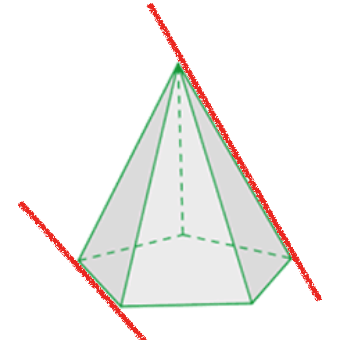
\includegraphics [width=0.45\textwidth ]{img-sol/t11-41}
 \end{enumerate}
\vspace{0.3cm}

 \needspace{4\baselineskip} 

{\textbf{\em Pàgina 145}} \hrulefill
\begin{enumerate}
\vspace{0.25cm}
\item[\fontfamily{phv}\selectfont\color{blue}\textbf{39. }] 
Solució gràfica: \par 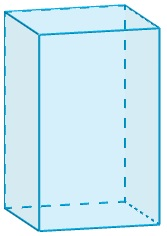
\includegraphics [width=0.45\textwidth ]{img-sol/prisma-cuadrangular}
 \end{enumerate}
\begin{enumerate}
\vspace{0.25cm}
\item[\fontfamily{phv}\selectfont\color{blue}\textbf{40. }] 
Ha de tenir 20 cares. Una piràmide convexa té tantes cares com vèrtexs, així que no pot ser una piràmide. Un prisma convex de 20 cares tindria dues bases i 18 cares laterals. En aquest cas hauria 54 arestes i 36 vèrtexs.
\vspace{0.25cm}
\item[\fontfamily{phv}\selectfont\color{blue}\textbf{41. }] 
Es pot construir un cub, un octàedre o dos tetraedres
\vspace{0.25cm}
\item[\fontfamily{phv}\selectfont\color{blue}\textbf{42. }] 
Té 10 cares. És un prisma octogonal.
\vspace{0.25cm}
\item[\fontfamily{phv}\selectfont\color{blue}\textbf{43. }] 
Con, Piràmide hexagonal regular. Compleix Euler, Piràmide pentagonal còncava. Compleix Euler, Poliedre format per 13 cares; 14 vèrtexs; 19 arestes. Compleix Euler
\vspace{0.25cm}
\item[\fontfamily{phv}\selectfont\color{blue}\textbf{44. }] 
En un prisma recte totes les cares laterals són rectangles; en l'oblic algunes no els són. Un prisma amb base un rombe o un romboide té quatre cares laterals que són rectangles paral·lels dos a dos i no és un ortoedre.
\vspace{0.25cm}
\item[\fontfamily{phv}\selectfont\color{blue}\textbf{45. }] 
Solució gràfica oberta
\vspace{0.25cm}
\item[\fontfamily{phv}\selectfont\color{blue}\textbf{46. }] 
$D=\sqrt {4^2+5^2+6^2}=8.77$ cm
\vspace{0.25cm}
\item[\fontfamily{phv}\selectfont\color{blue}\textbf{47. }] 
17 cm
\vspace{0.25cm}
\item[\fontfamily{phv}\selectfont\color{blue}\textbf{48. }] 
La diagonal d'aquest ortoedre mesura 13 cm. Si el bolígraf té diàmetre diferent de zero en les seves dues extrems, no hi cap.
\vspace{0.25cm}
\item[\fontfamily{phv}\selectfont\color{blue}\textbf{49. }] 
$D=2\sqrt {34}=11.7$ cm
\vspace{0.25cm}
\item[\fontfamily{phv}\selectfont\color{blue}\textbf{50. }] 
La diagonal de l'ortoedre mesura aproximadament 2.844 m. L'escala no hi cap.
\vspace{0.25cm}
\item[\fontfamily{phv}\selectfont\color{blue}\textbf{51. }] 
$2\sqrt {29}=10.77$ m
\vspace{0.25cm}
\item[\fontfamily{phv}\selectfont\color{blue}\textbf{52. }] 
Aproximadament 2 cm
\vspace{0.25cm}
\item[\fontfamily{phv}\selectfont\color{blue}\textbf{53. }] 
$\sqrt {149}=12.2$ cm
 \end{enumerate}
\vspace{0.3cm}

 \needspace{4\baselineskip} 

{\textbf{\em Pàgina 146}} \hrulefill
\begin{enumerate}
\vspace{0.25cm}


 \needspace{2\baselineskip} 

 \item[\fontfamily{phv}\selectfont\color{blue}\textbf{54}. ] 
 \begin{tasks}[column-sep=1em, item-indent=1.3333em](1)
	 \task Prisma quadrangular regular
	 \task Prisma hexagonal regular
	 \task Tronc d'un con
	 \task Tetraedre
\end{tasks}
 \end{enumerate}
\begin{enumerate}
\vspace{0.25cm}
\item[\fontfamily{phv}\selectfont\color{blue}\textbf{55. }] 
$A_L=96$ dm$^2$ i $A_T=108$ dm$^2$
\vspace{0.25cm}
\item[\fontfamily{phv}\selectfont\color{blue}\textbf{56. }] 
$A_B=24\sqrt {3}=41.57$ i $A_T=48(5+\sqrt {3})=323.14$ cm$^2$
\vspace{0.25cm}
\item[\fontfamily{phv}\selectfont\color{blue}\textbf{57. }] 
$V=360$ cm$^3$
\vspace{0.25cm}
\item[\fontfamily{phv}\selectfont\color{blue}\textbf{58. }] 
$A_T=232.9$ dm$^2$
\vspace{0.25cm}
\item[\fontfamily{phv}\selectfont\color{blue}\textbf{59. }] 
Atenció passa l'altura a cm! $A_T=8950\pi =28\,117.25$ cm$^2$ i $V=20\,000\pi =62\,831.85$ cm$^3$
\vspace{0.25cm}
\item[\fontfamily{phv}\selectfont\color{blue}\textbf{60. }] 
$A_T=100\pi =314.16$ cm$^2$
\vspace{0.25cm}
\item[\fontfamily{phv}\selectfont\color{blue}\textbf{61. }] 
$a_{piram}=\frac {4\sqrt {21}}{3}=6.11$ dm. $A_T=171.66$ dm$^2$; $V=\frac {512\sqrt {3}}{9}=98.53$ dm$^3$. On s'ha calculat també l'apotema de la base $a_{base}=4.6188$ dm i l'àrea de la base $A_B=73.9008$ dm$^2$
\vspace{0.25cm}
\item[\fontfamily{phv}\selectfont\color{blue}\textbf{62. }]  \scalebox{0.6}{\simbolclau } 
Apotema piràmide 4 m
\vspace{0.25cm}
\item[\fontfamily{phv}\selectfont\color{blue}\textbf{63. }] 
 Si l'eix de gir és el catet més gran:\par Àrea lateral: $65\pi = 204,20$ cm$^2$; àrea total: $90\pi = 282,74$ cm$^2$. Volum: $100\pi = 314,159$ cm$^3$.\par Si l'eix de gir és el catet menor:\par Àrea lateral: $156\pi = 480,09$ cm$^2$; àrea total: $300\pi = 942,48$ cm$^2$. Volum $240\pi =753,982$ cm$^3$
\vspace{0.25cm}
\item[\fontfamily{phv}\selectfont\color{blue}\textbf{64. }] 
$D=2\sqrt [3]{65755}=80.72$ dm
\vspace{0.25cm}
\item[\fontfamily{phv}\selectfont\color{blue}\textbf{65. }] 
$V=\frac {36\pi }{5}=22.619$ m$^3$ o $22\,619$ litres
\vspace{0.25cm}
\item[\fontfamily{phv}\selectfont\color{blue}\textbf{66. }] 
$A_T=100(1+\sqrt {26})=609.91$ cm$^2$
\vspace{0.25cm}
\item[\fontfamily{phv}\selectfont\color{blue}\textbf{67. }] 
$V=200\pi =628.319$ cm$^3$
\vspace{0.25cm}
\item[\fontfamily{phv}\selectfont\color{blue}\textbf{68. }] 
$A_B=\frac {31}{150}=0.206$ $m^2$ és a dir, té un radi de $R=\sqrt {\frac {0.206}{\pi }}=0.256$ m
\vspace{0.25cm}
\item[\fontfamily{phv}\selectfont\color{blue}\textbf{69. }] 
S'omplen $3 619 144$ envasos.
 \end{enumerate}
\vspace{0.3cm}

 \needspace{4\baselineskip} 

{\textbf{\em Pàgina 147}} \hrulefill
\begin{enumerate}
\vspace{0.25cm}
\item[\fontfamily{phv}\selectfont\color{blue}\textbf{70. }] 
Retallant tots els tetraedres, $A_T=40\sqrt {3}=69.28$ cm$^2$
 \end{enumerate}
\begin{enumerate}
\vspace{0.25cm}
\item[\fontfamily{phv}\selectfont\color{blue}\textbf{71. }] 
$A_T=48+2\sqrt {3}=51.46$ cm$^2$
\vspace{0.25cm}
\item[\fontfamily{phv}\selectfont\color{blue}\textbf{72. }] 
L'àrea total de la figura és $12+3\sqrt {3}=17.194$ m$^2$. Si el volem embolicar amb un rectangle de paper, ha de mesurar 6 m de llarg i 3.74 m d'ample. 
\vspace{0.25cm}
\item[\fontfamily{phv}\selectfont\color{blue}\textbf{73. }] 
$V=432\sqrt {3}=748.246$ dm$^3$ = litres. L'apotema de la base $a_p=51.96$ cm i l'àrea de la base $A_B=9353.074$ cm$^2$.
\vspace{0.25cm}
\item[\fontfamily{phv}\selectfont\color{blue}\textbf{74. }] 
Anomenam $r$ a la raó de proporcionalitat. Els costats són $3r$, $5r$ i $7r$. La diagonal és $\sqrt {9r^2+25r^2+49r^2}=14,5$. Obtenim $r=\frac {14,5}{\sqrt {83}}=1.592$. Llavors els costats reals són aproximadament: 4.776, 23.88 i 33.432. \par Amb aquestes dades, l'àrea total $A_T=360$ i el volum $V=423.66$
\vspace{0.25cm}
\item[\fontfamily{phv}\selectfont\color{blue}\textbf{75. }] 
$V=\frac {21-3\sqrt {33}}{4}=0.942$ dm$^3$
\vspace{0.25cm}
\item[\fontfamily{phv}\selectfont\color{blue}\textbf{76. }] 
$R=\sqrt {10}=3.2$ cm
\vspace{0.25cm}


 \needspace{2\baselineskip} 

 \item[\fontfamily{phv}\selectfont\color{blue}\textbf{77}. ] 
 \begin{tasks}[column-sep=1em, item-indent=1.3333em](1)
	 \task $V=3\pi =9.4247$ m$^3$
	 \task $9424.8$ litres
\end{tasks}
\vspace{0.25cm}


 \needspace{2\baselineskip} 

 \item[\fontfamily{phv}\selectfont\color{blue}\textbf{78}. ] 
 \begin{tasks}[column-sep=1em, item-indent=1.3333em](1)
	 \task $1$ l = $1000$ cm$^3$
	 \task l'altura és 10 cm (és un cub)
\end{tasks}
\vspace{0.25cm}
\item[\fontfamily{phv}\selectfont\color{blue}\textbf{79. }] 
Aproximadament 5,885 cm$^3$
\vspace{0.25cm}


 \needspace{2\baselineskip} 

 \item[\fontfamily{phv}\selectfont\color{blue}\textbf{80}. ] 
 \begin{tasks}[column-sep=1em, item-indent=1.3333em](1)
	 \task $0.064$ m$^3$
	 \task $219.2$ \euro {}
	 \task $19.2$ \euro {}
\end{tasks}
\vspace{0.25cm}
\item[\fontfamily{phv}\selectfont\color{blue}\textbf{81. }] 
$H=34.46$ m
\vspace{0.25cm}
\item[\fontfamily{phv}\selectfont\color{blue}\textbf{82. }] 
10 cm diàmetre i 10 cm d'altura. L'àrea són $100\pi =314.16$ cm$^2$
\vspace{0.25cm}
\item[\fontfamily{phv}\selectfont\color{blue}\textbf{83. }] 
 Àrea lateral: $500\pi \sqrt {26} = 8009.52$ cm$^2$.\par Si les bases són de vidre, mesuren respectivament $400\pi $ i $900\pi $. En total serien aproximadament $12093.59$ cm$^2$.
\vspace{0.25cm}
\item[\fontfamily{phv}\selectfont\color{blue}\textbf{84. }] 
Aproximadament $V=522.803$ cm$^3$
 \end{enumerate}
\vspace{0.3cm}

 \needspace{4\baselineskip} 

{\textbf{\em Pàgina 148}} \hrulefill
\begin{enumerate}
\vspace{0.25cm}
\item[\fontfamily{phv}\selectfont\color{blue}\textbf{85. }] 
$R=2$ dm
 \end{enumerate}
\begin{enumerate}
\vspace{0.25cm}


 \needspace{2\baselineskip} 

 \item[\fontfamily{phv}\selectfont\color{blue}\textbf{86}. ] 
 \begin{tasks}[column-sep=1em, item-indent=1.3333em](1)
	 \task 200 m$^3$=200\,000 litres
	 \task 4000 \euro {} 
\end{tasks}
\vspace{0.25cm}


 \needspace{2\baselineskip} 

 \item[\fontfamily{phv}\selectfont\color{blue}\textbf{87}. ]  \scalebox{0.6}{\simbolclau } 
 \begin{tasks}[column-sep=1em, item-indent=1.3333em](1)
	 \task* $A=480$ cm$^2$ i $V=448$ cm$^3$
	 \task* $A=226.19$ cm$^2$ i $V=282.743$ cm$^3$
	 \task* $A=$depèn de l'inclinació i $V=125.66$ cm$^3$
	 \task* $A=277.24$ cm$^2$ i $V=368.61$ cm$^3$
\end{tasks}
\vspace{0.25cm}
\item[\fontfamily{phv}\selectfont\color{blue}\textbf{88. }] 
Àrea de l'esfera $A=25\pi =78.54$ m$^2$. El cost és 23\,561.95 \euro {}.
\vspace{0.25cm}
\item[\fontfamily{phv}\selectfont\color{blue}\textbf{89. }] 
Ha costat 659.73 \euro {}
\vspace{0.25cm}
\item[\fontfamily{phv}\selectfont\color{blue}\textbf{90. }] 
El preu de la piràmide és 1\,294.29 \euro {}
\vspace{0.25cm}
\item[\fontfamily{phv}\selectfont\color{blue}\textbf{91. }] 
 Si fem coincidir els costats llargs, el volum és $\frac {9375}{\pi }=2984.15$ cm$^3$. Si fem coincidir els costats curts, el volum és $\dfrac {11250}{\pi }=3580.96$ cm$^3$. Aquest darrer és el major.
 \end{enumerate}
\vspace{0.3cm}

 \needspace{4\baselineskip} 

{\textbf{\em Pàgina 149}} \hrulefill
\begin{enumerate}
\vspace{0.25cm}


 \needspace{2\baselineskip} 

 \item[\fontfamily{phv}\selectfont\color{blue}\textbf{92}. ] 
 \begin{tasks}[column-sep=1em, item-indent=1.3333em](1)
	 \task* $A=274.45$ cm$^2$; $V=326.6$ cm$^3$
	 \task* $A=162.06$ cm$^2$; $V=116.64$ cm$^3$
	 \task* $A=124.71$ cm$^2$; $V=101.82$ cm$^3$
	 \task* $A=59.15$ dm$^2$; $V=41.6$ dm$^3$
\end{tasks}
 \end{enumerate}
\begin{enumerate}
\vspace{0.25cm}
\item[\fontfamily{phv}\selectfont\color{blue}\textbf{93. }] 
$V=48\pi =150.8$ dm$^3$
\vspace{0.25cm}
\item[\fontfamily{phv}\selectfont\color{blue}\textbf{94. }] 
En primer lloc hem de calcular el costat del quadrat $x$, per Pitàgores a l'espai $\sqrt {x^2+x^2+x^2}=103$ $\rightarrow $ $x=\frac {103}{\sqrt {3}}=59.47$ m. En segon lloc si l'escala és 1:100 simplement basta reemplaçar la unitat de metres per centímetres. Anem a calcular el volum total de la figura:\par $V=9 \times \frac {4}{3}\pi 9^3+4\times \pi 1^2 103 + 12 \times \pi 1^2 + 59.47 =9873.64 \pi = 31\,018.95$ cm$^3$ $=0.031$ m$^3$
\vspace{0.25cm}
\item[\fontfamily{phv}\selectfont\color{blue}\textbf{95. }] 
La campana circular $A_T=2\pi 20\cdot 40 + \pi \left [ 40\sqrt {40^2+150^2} - 20\sqrt {20^2+75^2} \right ]=6257.25\pi =19\,657.74$ cm$^2$ mentre que la campana rectangular $A_T=4\cdot 40\cdot 45 + 4 \cdot \frac {80+40}{2}\cdot 72.801=24\,672.24$. En aquest darrer cas hem hagut de cercar l'altura del trapezi lateral per Pitàgores que ha resultat esser $h=72.801$ cm.\par L'opció amb menys cost d'acer és la campana circular.
\vspace{0.25cm}
\item[\fontfamily{phv}\selectfont\color{blue}\textbf{96. }] 
17 cubs
\vspace{0.25cm}
\item[\fontfamily{phv}\selectfont\color{blue}\textbf{97. }] 
$V=\frac {261\pi }{8}=102.49$ cm$^3$= $10.249$ cl
\vspace{0.25cm}
\item[\fontfamily{phv}\selectfont\color{blue}\textbf{98. }] 
$V=\frac {11314 \pi }{3}=11\,847.993$ cm$^3$
\vspace{0.25cm}
\item[\fontfamily{phv}\selectfont\color{blue}\textbf{99. }] 
L'ombra és igual al octògon de la base. L'àrea d'un octògon de costat $a$ és $A=\frac {2a^2}{\sqrt {3-2\sqrt {2}}}$. Fent que $a=45$ cm, obtenim l'àrea aproximada és de $9\,777.56$ cm$^2$.
 \end{enumerate}
\vspace{0.3cm}

 \needspace{4\baselineskip} 

{\textbf{\em Pàgina 150}} \hrulefill
\begin{enumerate}
\vspace{0.25cm}
\item[\fontfamily{phv}\selectfont\color{blue}\textbf{100. }] 
$V=\frac {16000\pi }{81}=877.607$ cm$^3$.
 \end{enumerate}
\begin{enumerate}
\vspace{0.25cm}
\item[\fontfamily{phv}\selectfont\color{blue}\textbf{101. }] 
$H=\frac {60}{\pi }=19,2$ cm
\vspace{0.25cm}
\item[\fontfamily{phv}\selectfont\color{blue}\textbf{102. }] 
$H=\frac {360}{\pi }=114.6$ cm
\vspace{0.25cm}
\item[\fontfamily{phv}\selectfont\color{blue}\textbf{103. }] 
$H=\frac {875}{27}=32.41$ cm
\vspace{0.25cm}
\item[\fontfamily{phv}\selectfont\color{blue}\textbf{104. }] 
Veure problema anterior. Aquest està repetit.
\vspace{0.25cm}
\item[\fontfamily{phv}\selectfont\color{blue}\textbf{105. }] 
$A_T=2 A_B + A_L = 2 \pi (3^2-2^2) + 2\pi 10 (3+2)=110\pi =345.58$ m$^2$ i $V=\pi (3^2-2^2)\cdot 10=157.08$ m$^3$
\vspace{0.25cm}
\item[\fontfamily{phv}\selectfont\color{blue}\textbf{106. }] 
Superfície de galeta: $\frac {25\pi \sqrt {37}}{4} = 119,43$ cm$^2$. El volum de gelat és $\frac {125\pi }{4} = 98,175$ cm$^3$. La massa depèn de la densitat del gelat. 
\vspace{0.25cm}
\item[\fontfamily{phv}\selectfont\color{blue}\textbf{107. }] 
Té $75^\circ $ de longitud. De la latitud no en sabem rés.
\vspace{0.25cm}
\item[\fontfamily{phv}\selectfont\color{blue}\textbf{108. }] 
A les 16 hores.
\vspace{0.25cm}
\item[\fontfamily{phv}\selectfont\color{blue}\textbf{109. }] 
És deu a la diferència de latitud entre els dos llocs.
 \end{enumerate}
\vspace{0.3cm}

 \needspace{4\baselineskip} 

{\textbf{\em Pàgina 151}} \hrulefill
\begin{enumerate}
\vspace{0.25cm}
 \item[$\bullet$ ] {\fontfamily{phv}\selectfont\color{blue}\textbf{Autoavaluació:}. }

 \end{enumerate}
\begin{enumerate}
\vspace{0.25cm}
\item[\fontfamily{phv}\selectfont\color{blue}\textbf{1. }]  \scalebox{0.6}{\simbolclau } 
\textbf {--9.} Autoavaluació: 1c; 2a; 3d; 4b; 5a; 6d; 7b; 8a; 9c.
 \end{enumerate}
\vspace{0.3cm}

 \needspace{4\baselineskip} 

{\textbf{\em Pàgina 152}} \hrulefill
\begin{enumerate}
\vspace{0.25cm}
 \item[$\bullet$ ] {\fontfamily{phv}\selectfont\color{blue}\textbf{Autoavaluació:}. }

 \end{enumerate}
\vfill\null
\columnbreak
\def\currentname{Solucions del Tema 12}
\vspace*{0.75cm}

 
 \needspace{5\baselineskip} 
 \scalebox{1.25}{\heading{Solucions del Tema 12}}

\vspace*{0.4cm}
\phantomsection \addcontentsline{toc}{section}{Solucions del Tema 12}
\vspace{0.3cm}

 \needspace{4\baselineskip} 

{\textbf{\em Pàgina 156}} \hrulefill
\begin{enumerate}
\vspace{0.25cm}
\item[\fontfamily{phv}\selectfont\color{blue}\textbf{1. }]  \scalebox{0.6}{\simbolclau } 
 a) $\frac {-5}{12}$;\quad b) $\frac {-3}{7}$
 \end{enumerate}
\begin{enumerate}
\vspace{0.25cm}
\item[\fontfamily{phv}\selectfont\color{blue}\textbf{2. }]  \scalebox{0.6}{\simbolclau } 
 $5^{20}$
\vspace{0.25cm}
\item[\fontfamily{phv}\selectfont\color{blue}\textbf{3. }]  \scalebox{0.6}{\simbolclau } 
a) 29 exercicis dia 15; \par b) 225 exercicis en total.
\vspace{0.25cm}
\item[\fontfamily{phv}\selectfont\color{blue}\textbf{4. }]  \scalebox{0.6}{\simbolclau } 
 a) $N=25$; $\sum f_i x_i = 41$; $\sum f_i x_i^2 =83$;\par c) $Mo=2$; $\bar x=1,64$; $\sigma =0,79$; $CV=0,48$ (48 \%).
\vspace{0.25cm}
\item[\fontfamily{phv}\selectfont\color{blue}\textbf{5. }]  \scalebox{0.6}{\simbolclau } 
 a) 0,51; b) 0,42
 \end{enumerate}
\vspace{0.3cm}

 \needspace{4\baselineskip} 

{\textbf{\em Pàgina 157}} \hrulefill
\begin{enumerate}
\vspace{0.25cm}
\item[\fontfamily{phv}\selectfont\color{blue}\textbf{6. }]  \scalebox{0.6}{\simbolclau } 
 a) $3x^4+5x^3+2x^2-2x-4$; \par b) $3x^4+9x^3-8x^2+10x-5$; \par c) $-4x^4+4x^3+x^2-23x-3$; \par d) $4x^2+12x+9$
 \end{enumerate}
\begin{enumerate}
\vspace{0.25cm}
\item[\fontfamily{phv}\selectfont\color{blue}\textbf{7. }]  \scalebox{0.6}{\simbolclau } 
 a) $x=1,82$ i $x=-0,82$; \par b) $x=-1$ i $x=5$
\vspace{0.25cm}
\item[\fontfamily{phv}\selectfont\color{blue}\textbf{8. }]  \scalebox{0.6}{\simbolclau } 
 $x=-3$ i $y=7$
\vspace{0.25cm}
\item[\fontfamily{phv}\selectfont\color{blue}\textbf{9. }]  \scalebox{0.6}{\simbolclau } 
 Consumeixen $3000$ kWh
\vspace{0.25cm}
\item[\fontfamily{phv}\selectfont\color{blue}\textbf{10. }]  \scalebox{0.6}{\simbolclau } 
 $y=0.30 \cdot x + 100$; \quad $y=190$ €; \quad $x=65$ km
\vspace{0.25cm}
\item[\fontfamily{phv}\selectfont\color{blue}\textbf{11. }]  \scalebox{0.6}{\simbolclau } 
 Paràbola convexa en vèrtex al punt $x=5/2$, $y=17/4$
\vspace{0.25cm}
\item[\fontfamily{phv}\selectfont\color{blue}\textbf{12. }]  \scalebox{0.6}{\simbolclau } 
 $1.8585\cdots = \frac {184}{99}$ i $2.888 \cdots = \frac {26}{9}$. La mitjana és $x=\frac {235}{99}$. 
\vspace{0.25cm}
\item[\fontfamily{phv}\selectfont\color{blue}\textbf{13. }]  \scalebox{0.6}{\simbolclau } 
 947,37 \euro {} \ de sou brut
\vspace{0.25cm}
\item[\fontfamily{phv}\selectfont\color{blue}\textbf{14. }]  \scalebox{0.6}{\simbolclau } 
 a) $2,47\cdot 10^{-6}$ \quad b) $0,43943\cdots $ \quad c) 5 cm perquè $5^{3}$=125
\vspace{0.25cm}
\item[\fontfamily{phv}\selectfont\color{blue}\textbf{15. }]  \scalebox{0.6}{\simbolclau } 
 Per exemple, 17 anys = $5,36\cdot 10^{8}$ s
\vspace{0.25cm}
\item[\fontfamily{phv}\selectfont\color{blue}\textbf{16. }]  \scalebox{0.6}{\simbolclau } 
El dia 21 va nadar 115 minuts; durant els 21 dies va nadar 1365 minuts.
 \end{enumerate}
\vspace{0.3cm}

 \needspace{4\baselineskip} 

{\textbf{\em Pàgina 158}} \hrulefill
\begin{enumerate}
\vspace{0.25cm}
\item[\fontfamily{phv}\selectfont\color{blue}\textbf{17. }]  \scalebox{0.6}{\simbolclau } 
 a) 38 hotels; c) mitjana=2.47; desv. típica=0.88; C.V. = 0.36 (36\%)
 \end{enumerate}
\begin{enumerate}
\vspace{0.25cm}
\item[\fontfamily{phv}\selectfont\color{blue}\textbf{18. }]  \scalebox{0.6}{\simbolclau } 
 a) grau 4; \quad b) $7x^{3}$; \quad c) 2 $x^{2}-4x$
\vspace{0.25cm}
\item[\fontfamily{phv}\selectfont\color{blue}\textbf{19. }]  \scalebox{0.6}{\simbolclau } 
 $P=6/11 \approx 0,54$
\vspace{0.25cm}
\item[\fontfamily{phv}\selectfont\color{blue}\textbf{20. }]  \scalebox{0.6}{\simbolclau } 
 $x=2y$; $x -8 = y+8$; \quad 3r A: $x= 32$; \quad 3r B: $y=16$.
\vspace{0.25cm}
\item[\fontfamily{phv}\selectfont\color{blue}\textbf{21. }]  \scalebox{0.6}{\simbolclau } 
 a) No té solució; \quad b) $x=-3$ i $x=3$; \par c) $x=0$ i $x=-2$; \quad d) $x=1$ i $x=-3$
\vspace{0.25cm}
\item[\fontfamily{phv}\selectfont\color{blue}\textbf{22. }]  \scalebox{0.6}{\simbolclau } 
 $x+30=\frac {x^2}{5}$; $x^2-5x-150=0$ $\rightarrow $ $x=-10$ no val; $x=15$ anys.
\vspace{0.25cm}
\item[\fontfamily{phv}\selectfont\color{blue}\textbf{23. }]  \scalebox{0.6}{\simbolclau } 
 Gastaran 672 \euro {} 
\vspace{0.25cm}
\item[\fontfamily{phv}\selectfont\color{blue}\textbf{24. }]  \scalebox{0.6}{\simbolclau } 
Ajuda: Utilitza l'equació de la funció lineal y= mx+n. Determina m i n. a) $y=-\frac {2}{3}x\ +\ 12$ ; \quad b) $\ 5=-\frac {2}{3}x\ +\ 12$ $\rightarrow $ $x=10,5$ hores
 \end{enumerate}
\vspace{0.3cm}

 \needspace{4\baselineskip} 

{\textbf{\em Pàgina 159}} \hrulefill
\begin{enumerate}
\vspace{0.25cm}
\item[\fontfamily{phv}\selectfont\color{blue}\textbf{25. }]  \scalebox{0.6}{\simbolclau } 
 a) $y=3x+600$; \par b) $\mathrm {1230}\mathrm {\ }=3x+600$ $\rightarrow $ $x=210$ kg de taronges
 \end{enumerate}
\begin{enumerate}
\vspace{0.25cm}
\item[\fontfamily{phv}\selectfont\color{blue}\textbf{26. }]  \scalebox{0.6}{\simbolclau } 
 a) Lineal creixent; \quad b) paràbola còncava, $V(0,1)$; \quad Lineal decreixent
\vspace{0.25cm}


 \needspace{2\baselineskip} 

 \item[\fontfamily{phv}\selectfont\color{blue}\textbf{27}. ]  \scalebox{0.6}{\simbolclau } 
 \begin{tasks}[column-sep=1em, item-indent=1.3333em](1)
	 \task* Creix a (0,\,4) i (9,\,12) i (15,\,19) min.; Decreix a (4,\,9) i (12,\,12) i (19,\,21) min.
	 \task 1 min; 20.5 min
	 \task* Màxim 45 km/h als 4 minuts i Mínima de 15 km/h als 9 min.
	 \task* És una funció contínua. El domini és (0,\,21) i el recorregut (0,\,45) 
\end{tasks}
\vspace{0.25cm}
\item[\fontfamily{phv}\selectfont\color{blue}\textbf{28. }]  \scalebox{0.6}{\simbolclau } 
No perquè $\dfrac {15}{10} \neq \dfrac { 65}{60}$. Només podríem dibuixar 13 cm dels 15 cm de la fotografia.
\vspace{0.25cm}
\item[\fontfamily{phv}\selectfont\color{blue}\textbf{29. }]  \scalebox{0.6}{\simbolclau } 
$h=2,9$ cm
\vspace{0.25cm}
\item[\fontfamily{phv}\selectfont\color{blue}\textbf{30. }]  \scalebox{0.6}{\simbolclau } 
$A=36$ cm$^2$, $A=32$ cm$^2$, $A=377$ cm$^2$
 \end{enumerate}
\vspace{0.3cm}

 \needspace{4\baselineskip} 

{\textbf{\em Pàgina 160}} \hrulefill
\begin{enumerate}
\vspace{0.25cm}


 \needspace{2\baselineskip} 

 \item[\fontfamily{phv}\selectfont\color{blue}\textbf{31}. ]  \scalebox{0.6}{\simbolclau } 
 \begin{tasks}[column-sep=1em, item-indent=1.3333em](1)
	 \task $A'(4,0)$ $B'(5,-2)$ $C'(6,2)$
	 \task* $A'(1,-2)$ $B'(2,0)$ $C'(3,-4)$
	 \task* $A'(-2,1)$ $B'(0,2)$ $C'(-4,3)$
	 \task $A'(5,6)$ $B'(7,5)$ $C'(3,4)$
\end{tasks}
 \end{enumerate}
\begin{enumerate}
\vspace{0.25cm}
\item[\fontfamily{phv}\selectfont\color{blue}\textbf{32. }]  \scalebox{0.6}{\simbolclau } 
$A_T =13,88$ hm$^{2}$, $V=2,59$ hm$^3$
\vspace{0.25cm}
\item[\fontfamily{phv}\selectfont\color{blue}\textbf{33. }]  \scalebox{0.6}{\simbolclau } 
$A_T =547,06$ cm$^{2}$, $V=935,3$ cm$^3$
\vspace{0.25cm}
\item[\fontfamily{phv}\selectfont\color{blue}\textbf{34. }]  \scalebox{0.6}{\simbolclau } 
$A=50\sqrt {3}$ cm$^{2}$, $V=V_{cub} -V_{piram}=250$ cm$^{3}$
\vspace{0.25cm}
\item[\fontfamily{phv}\selectfont\color{blue}\textbf{35. }]  \scalebox{0.6}{\simbolclau } 
$V=338,7$ cm$^3$
\vspace{0.25cm}
\item[\fontfamily{phv}\selectfont\color{blue}\textbf{36. }]  \scalebox{0.6}{\simbolclau } 
Hem de posar 1.54 kg de pH+ per augmentar 0.4 punts.
 \end{enumerate}
\end{multicols}
\end{document}